% !TEX root = mythesis.tex

%==============================================================================
\chapter{Results}
\label{chap:results}


In this chapter, the results of the fit is presented. In order to assess the results of the fit, comparisons between the pre-fit and post-fit plots, event yields and uncertainties are studied. 

Section \ref{sec:ecpectedfitresults} summarises the expected fit results that are obtained by performing the binned likelihood fit on the Asimov data. The Asimov data is the one in which all observed quantities are equal to their expected values In section \ref{sec:observedfitresults}, the results of the fit performed on the data is presented. Section \ref{sec:discussionoftheresults} presents a discussion of the gives, including a brief comparison with the recent tZq cross-section measurement published by both ATLAS and CMS experiment.


%==============================================================================

\section{Expected fit results}
\label{sec:ecpectedfitresults}

The expected fit results are the one that are obtained by performing the  Asimov fit. Before performing the Asmiov fit, a fit is performed in the signal depleted region to get the nominal values of three backgrounds NormFactors. SRs with $O_{NN}<0.4$, CRs $t\Bar{t}Z$ with $O_{NN}<0.6$ and other CRs remaining intact is fitted on the unblinded dataset.

\begin{figure}[!h] 
  \begin{subfigure}[b]{0.49\linewidth}
    \centering
    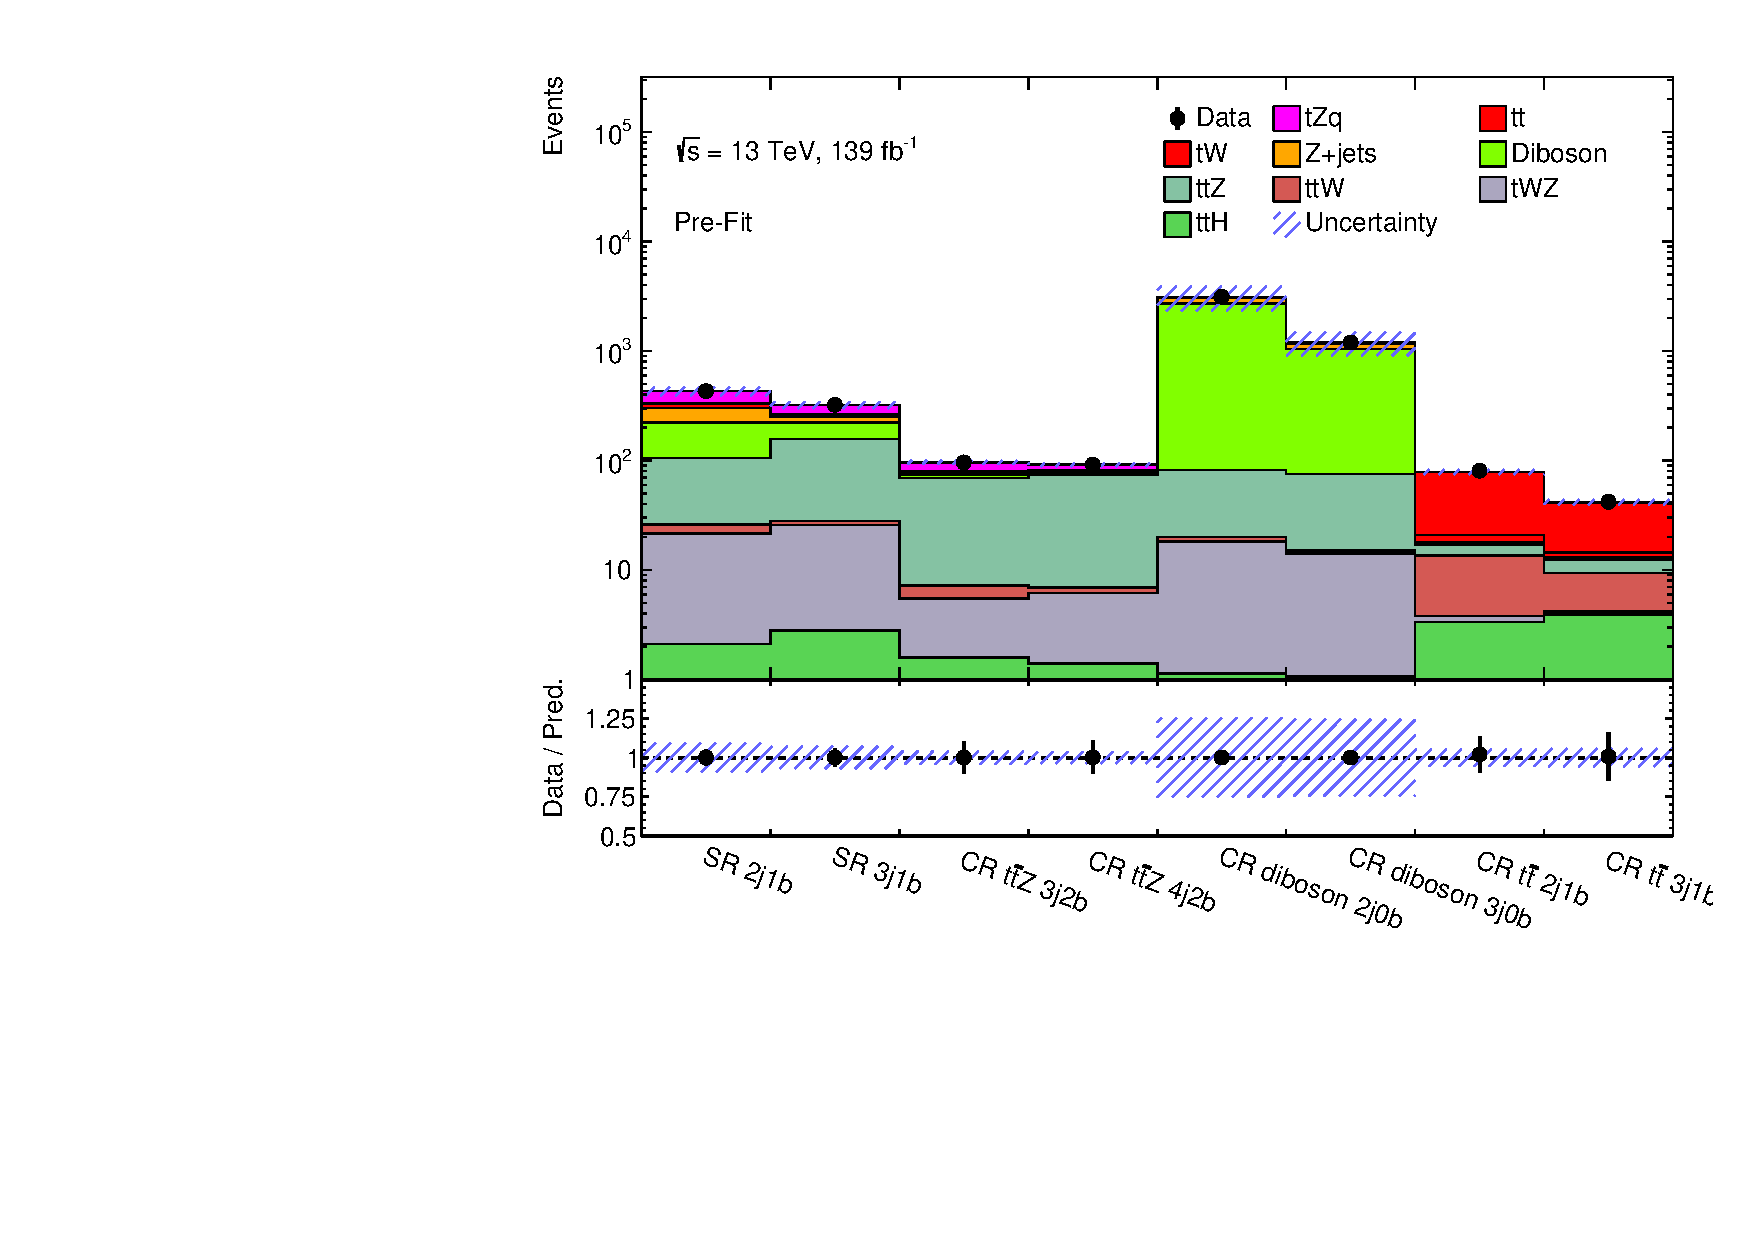
\includegraphics[width=\textwidth]{ubonn-thesis/Chapters/Chapters_07/Figure/Asmiov/Summary.pdf}
    \caption{}
  \end{subfigure}%% 
  \begin{subfigure}[b]{0.49\linewidth}
    \centering
    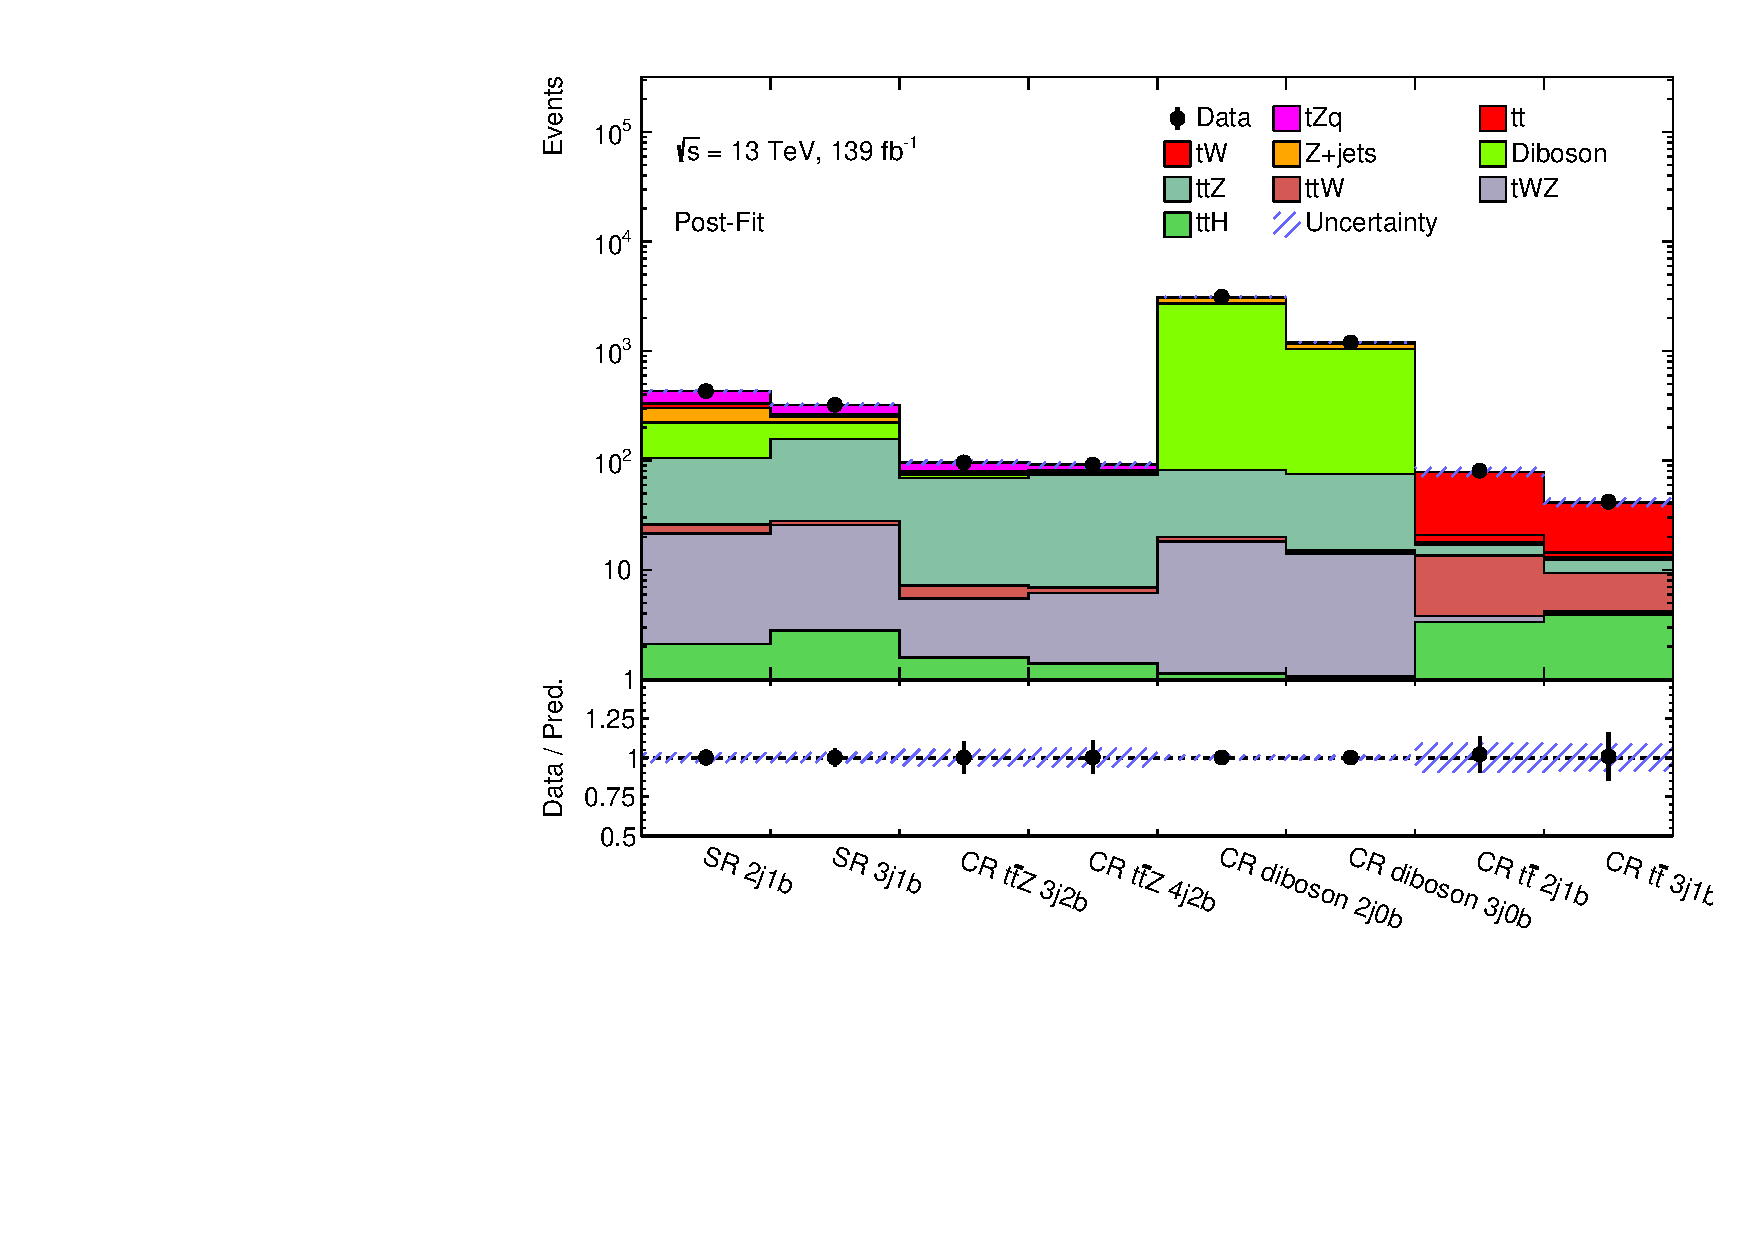
\includegraphics[width=\textwidth]{ubonn-thesis/Chapters/Chapters_07/Figure/Asmiov/Summary_postFit.pdf}
   \caption{}
  \end{subfigure}
  \caption{Summary plot of events in the signal and control regions during the Asimov fit. The implemented Asimov fit is a hybrid one. (a) Pre-fit plot (b) Post-fit plot }
  \label{fig:summaryplot}
\end{figure}


\begin{figure}[!h] 
  \begin{subfigure}[b]{0.49\linewidth}
    \centering
    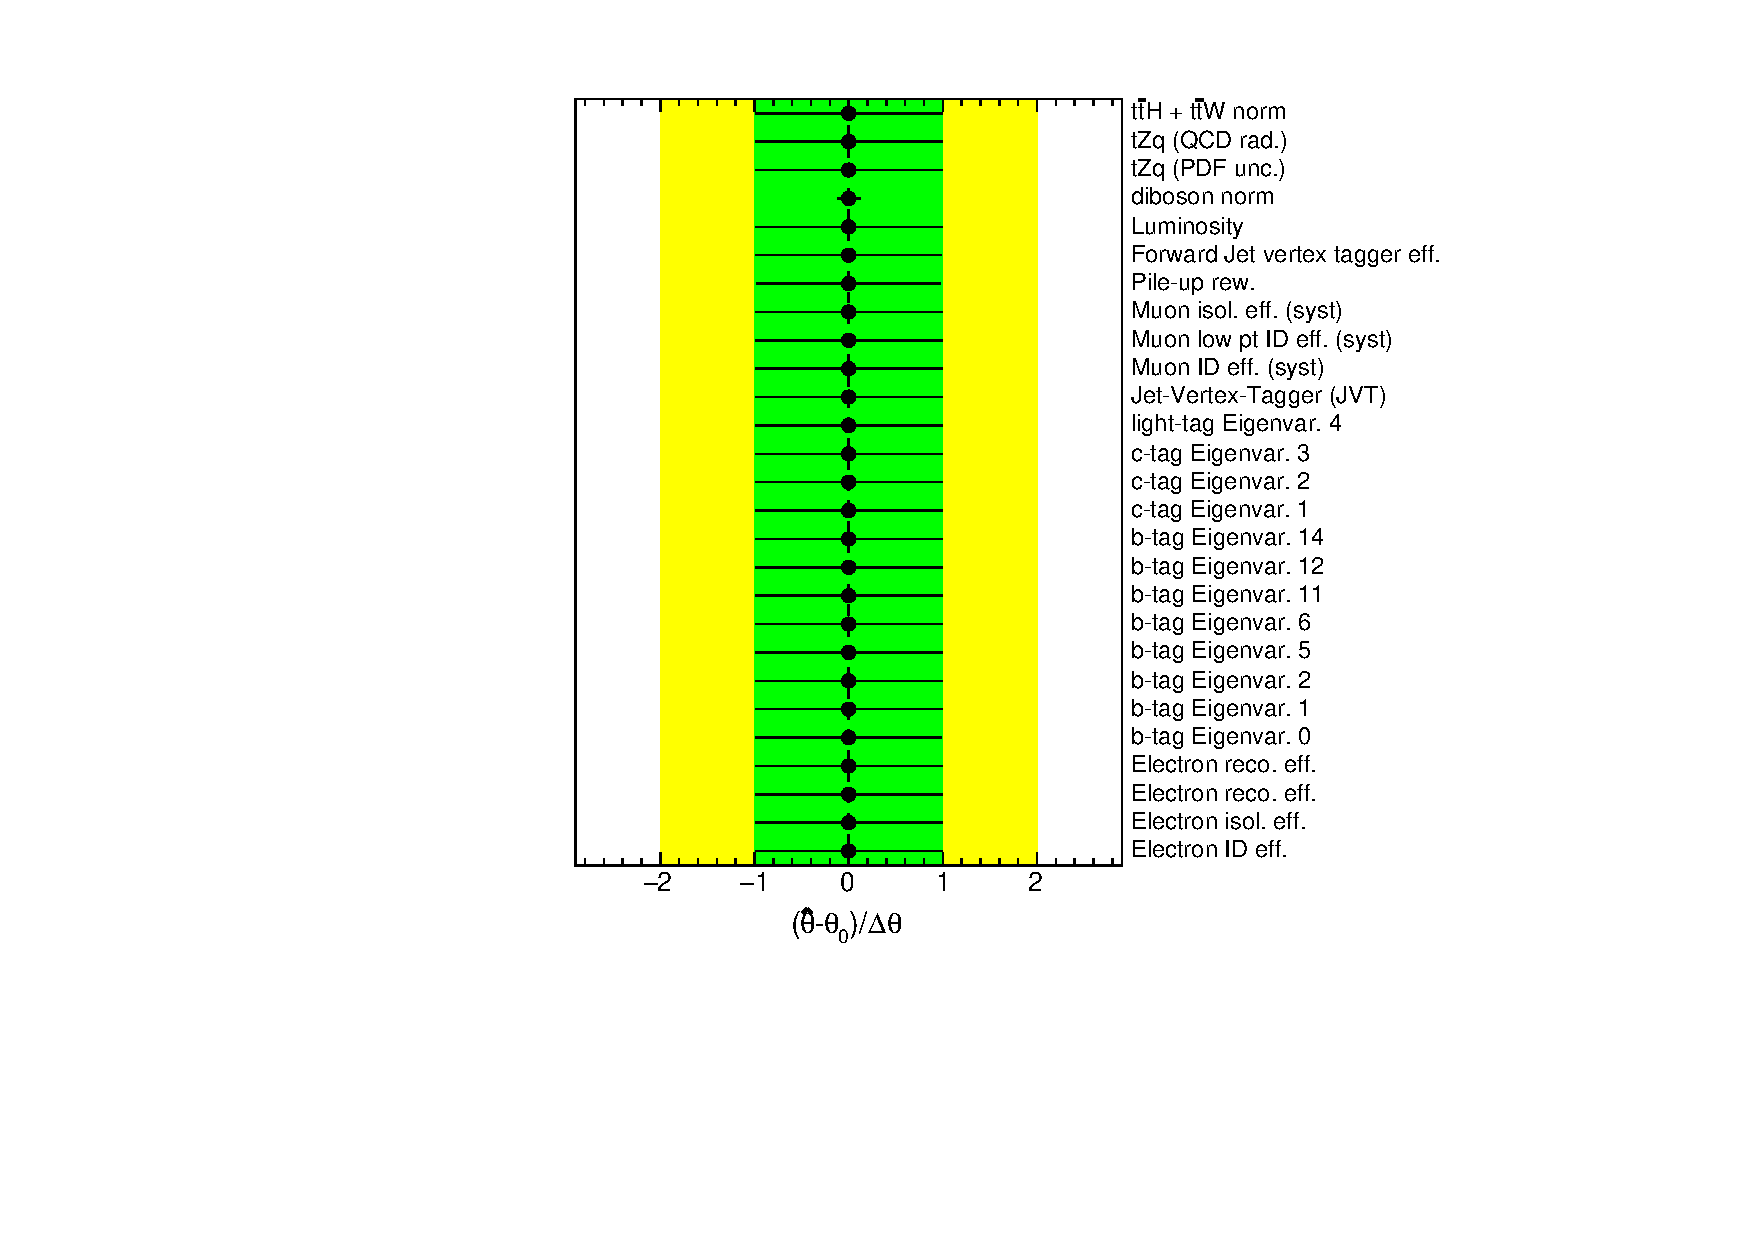
\includegraphics[width=1.24\textwidth]{ubonn-thesis/Chapters/Chapters_07/Figure/Asmiov/NuisPar.pdf}
    \caption{}
    \label{fig:asimovpull}
  \end{subfigure}%% 
  \begin{subfigure}[b]{0.49\linewidth}
    \centering
    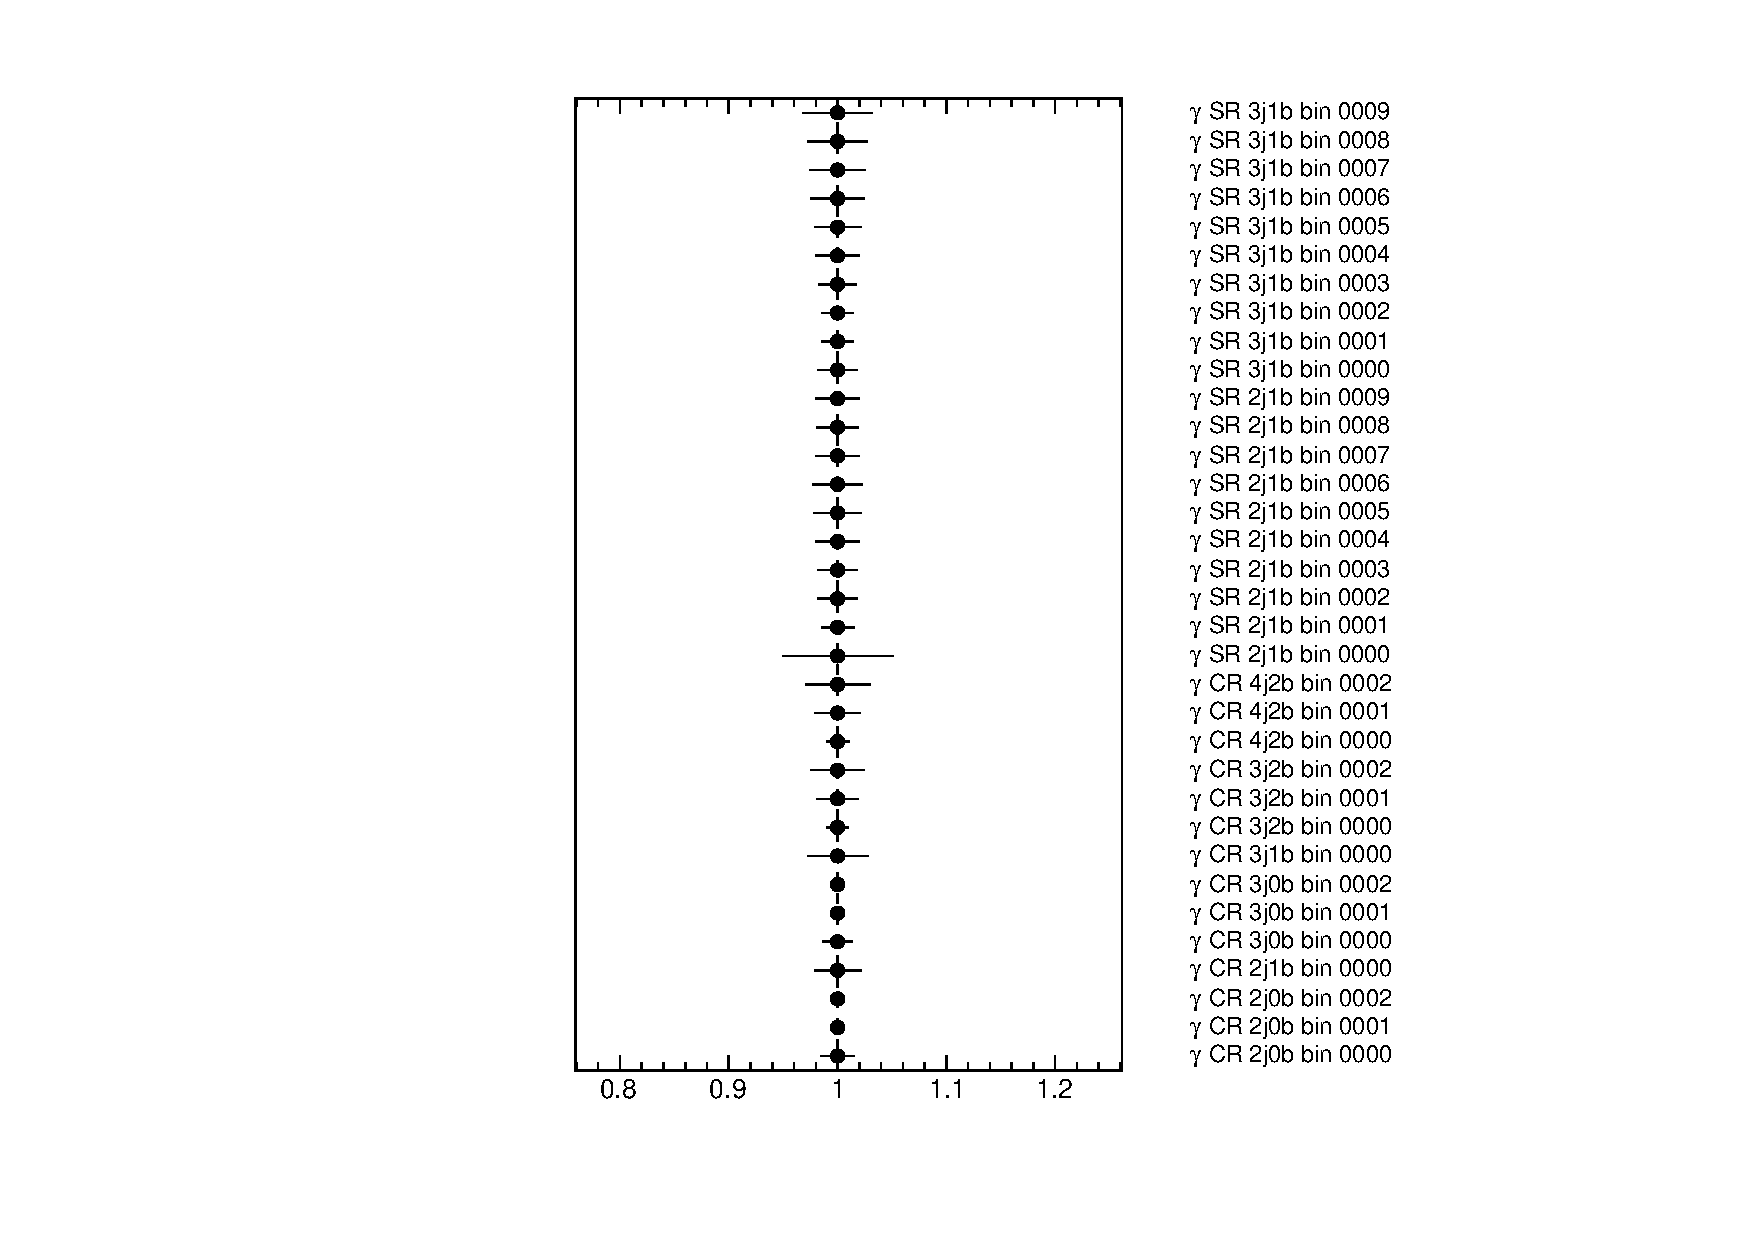
\includegraphics[width=1.1\textwidth]{ubonn-thesis/Chapters/Chapters_07/Figure/Asmiov/Gammas.pdf}
   \caption{}
   \label{fig:asimovgamma}
  \end{subfigure}
  \caption{(a) Pull distributions of nuisance parameters associated to systematic uncertainties using the blinded dataset. Only nuisance parameters substantial effect are shown. (b) Pull distributions of bin gamma parameters in the blinded fit.}
\end{figure}

\begin{figure}[!h] 
  \begin{subfigure}[b]{0.49\linewidth}
    \centering
    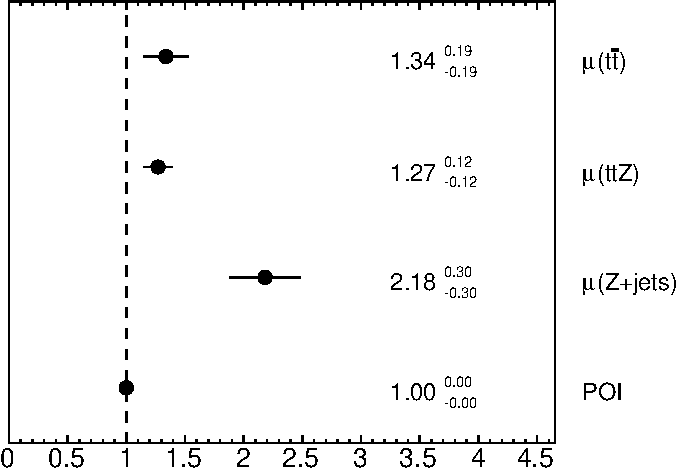
\includegraphics[width=\textwidth]{ubonn-thesis/Chapters/Chapters_07/Figure/Asmiov/NormFactors_bkg-crop.pdf}
    \caption{}
    \label{fig:backgroundonly}
  \end{subfigure}%% 
  \begin{subfigure}[b]{0.49\linewidth}
    \centering
    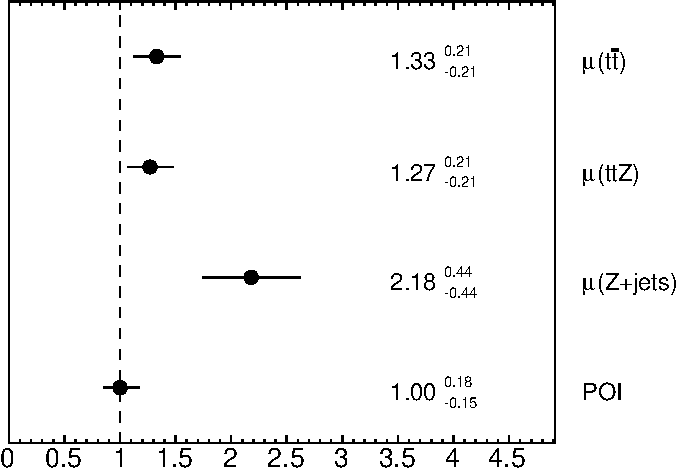
\includegraphics[width=\textwidth]{ubonn-thesis/Chapters/Chapters_07/Figure/Asmiov/NormFactors-crop.pdf}
   \caption{}
   \label{fig:asimovnormfactor}
  \end{subfigure}
  \caption{(a) Norm factors of the free floating parameters in the fit performed in the signal depleted regions using unblineded dataset.  and (b) Norm factors of the free floating parameters used in the signal plus background fit using blinded dataset.}
\end{figure}

\begin{figure}[!h] 
  \begin{subfigure}[b]{0.49\linewidth}
    \centering
    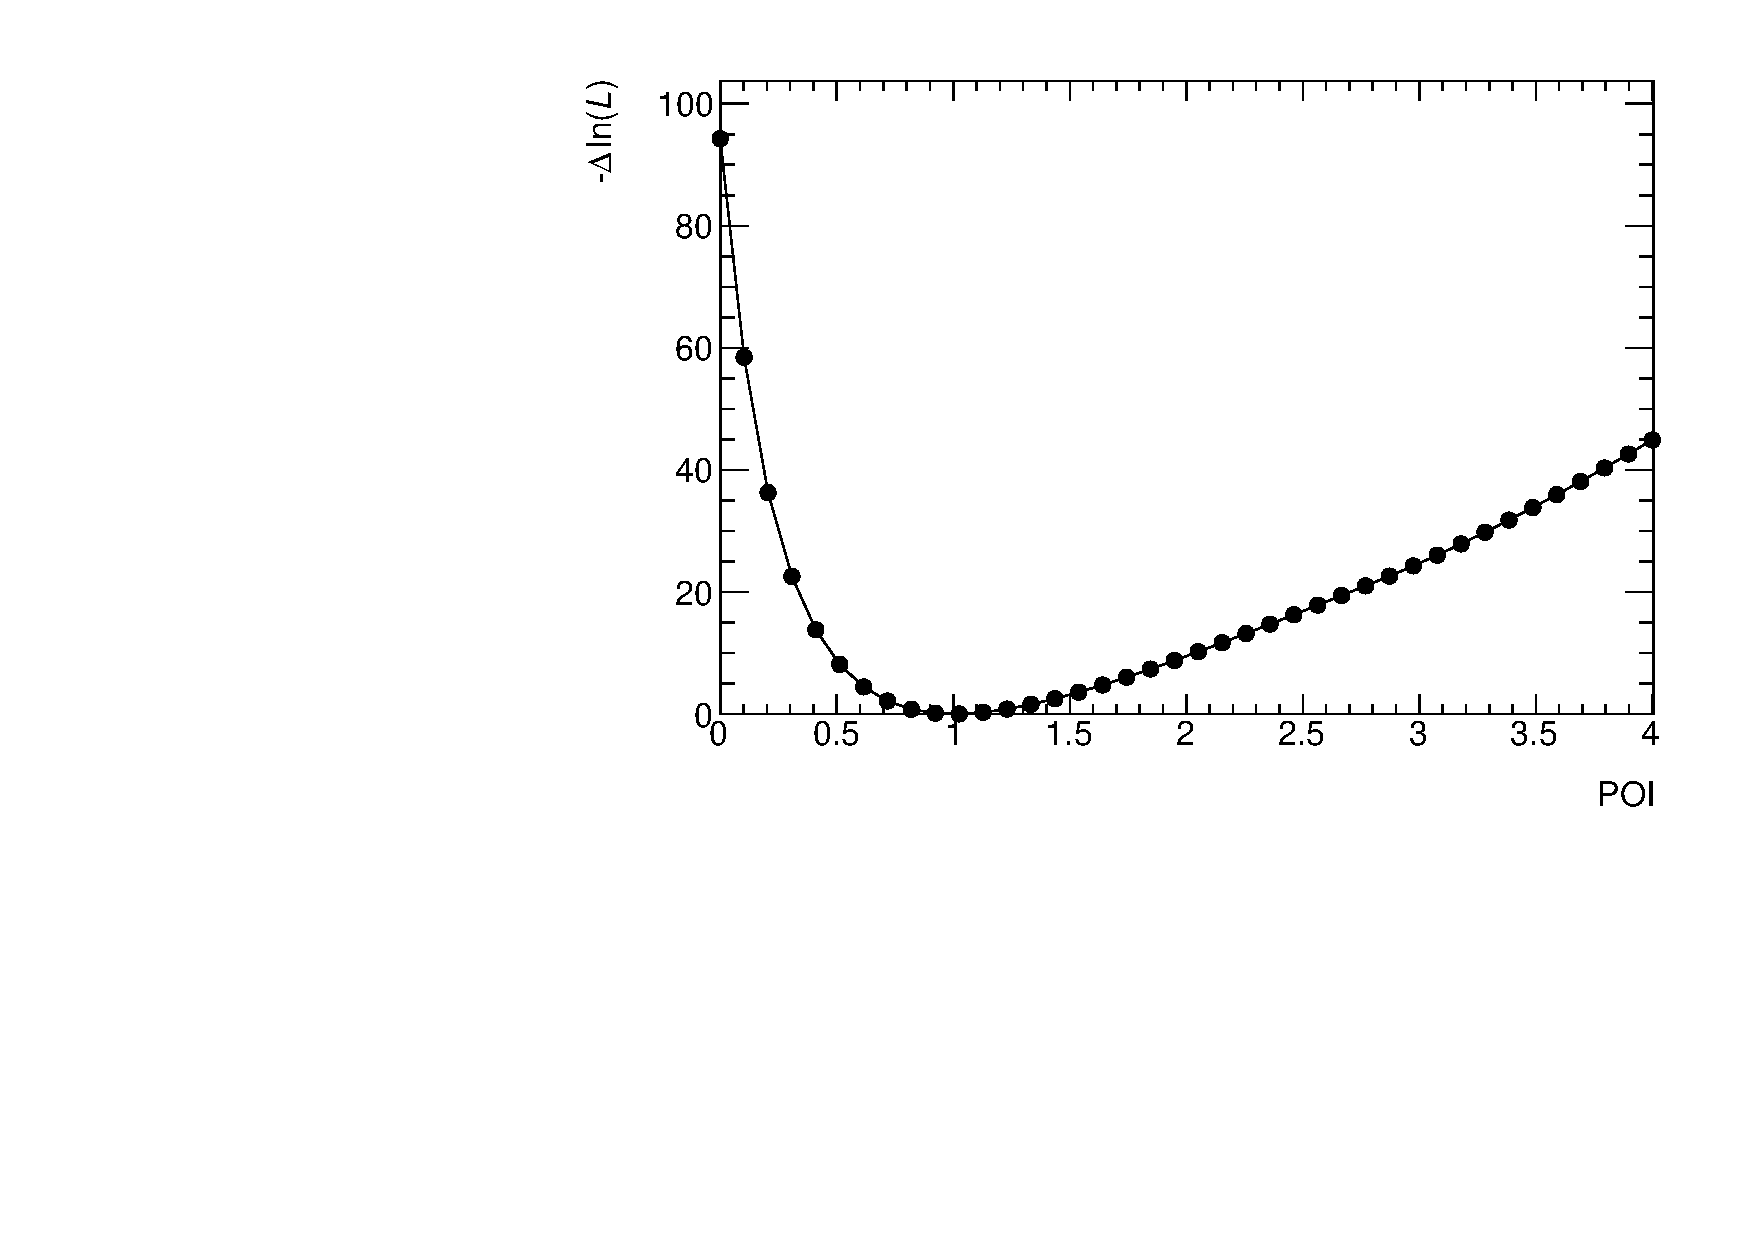
\includegraphics[width=\textwidth]{ubonn-thesis/Chapters/Chapters_07/Figure/Asmiov/NLLscan_POI.pdf}
    \caption{}
    \label{fig:asimovNLL}
  \end{subfigure}%% 
  \begin{subfigure}[b]{0.49\linewidth}
    \centering
    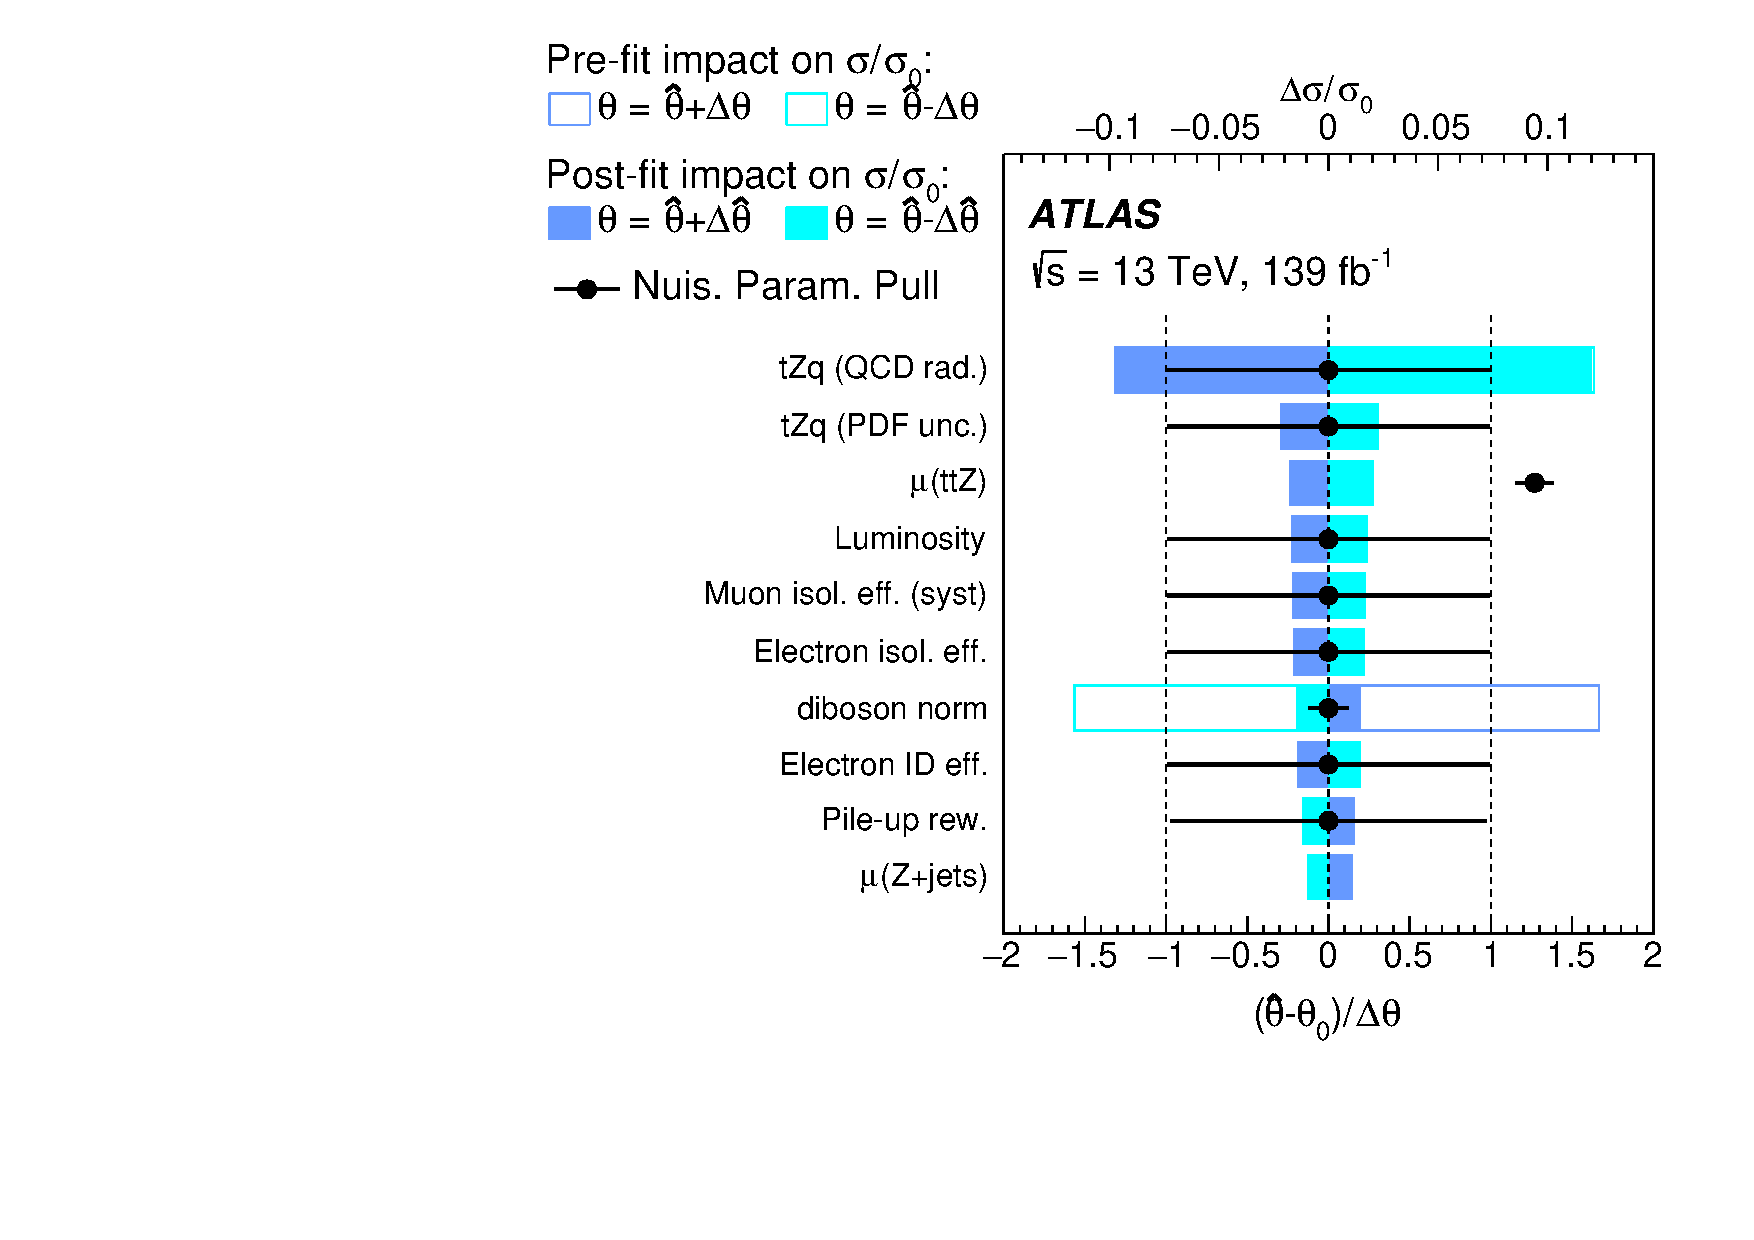
\includegraphics[width=\textwidth]{ubonn-thesis/Chapters/Chapters_07/Figure/Asmiov/RankingSysts_POI_systs.pdf}
   \caption{}
   \label{fig:ranking_asimov_R}
  \end{subfigure}
  \caption{(a) The likelihood scan of the signal strength ($\mu$) or parameter of interest (POI) and (b) The ranking plot showing the impact of each NP on $\mu$ in the Asimov fit. There, the empty/full boxes show the pre-/post-fit impacts while the black dots/lines represent the post-fit values/uncertainties of all NPs. Only the 10 NPs with the highest post-fit impacts are displayed.}
  \label{fig:ranking_asimov}
\end{figure}

 The result of the background only fit is shown in figure \ref{fig:backgroundonly}. The obtained Norm factors are used as the nominal values for the blinded and unblinded fit.

Asimov fit is a test fit performed on the pseudo data, where the combination of predicted background and signal assuming a signal strength of $\mu = 1$, is used. The nominal distributions are used to create this dataset i.e. all the NPs are set to zero in the Asimov fit and exactly matches signal plus background hypothesis as shown in figure \ref{fig:summaryplot}. The post-fit values (pulls) of all NPs have to be close to zero while the post-fit uncertainties can be smaller than their pre-fit uncertainties due to constrain on uncertainties. The result is $\mu =1$, which corresponds to an expected uncertainty of 18\% as shown in figure \ref{fig:asimovnormfactor}. The total uncertainties include both the statistical and the systematic uncertainties. The post-fit values of all the NPs are shown in figure \ref{fig:asimovpull} and all are centered around zero. The pull of the gammas is shown in figure \ref{fig:asimovgamma}.

In order to check the stability, the likelihood scan of the signal strength ($\mu$) is performed. The resulting (minimised) negative log-likelihood plot is shown in figure \ref{fig:asimovNLL}. The curve has a very smooth and parabolic shape which says that the fit configuration is stable and results are reliable. The norm factors of the Asimov fit is shown in figure \ref{fig:asimovnormfactor}. To get an idea of which NPs have the largest impact on the fitted signal strength, their ranking is investigated, which is shown in figure \ref{fig:ranking_asimov_R}. It can be concluded that the uncertainty on the signal strength is dominated by the tZq QCD radiation uncertainties.  


\section{Observed fit results}
\label{sec:observedfitresults}

The fit configuration that was tested on pseudo data in the previous section, is used to fit the observed full Run II data in order to extract the signal strength and thereby the cross-section. The pre-fit and post-fit of the fitted distributions in the signal and control regions are shown in figures \ref{fig:datafit1} and \ref{fig:datafit2}. Comparing to the pre-fit  and post-fit distributions in figures  \ref{fig:datafit1} and \ref{fig:datafit2}, one can observe that the agreement with data is significantly improved. The corresponding p-value of $\chi^{2}-$test between the data and MC samples are shown in the ratio plots. For all fit regions, the p-value is above 0.05. Also, the total uncertainty is significantly reduced after fit. 

\begin{figure}[!h] 
  \begin{subfigure}[b]{0.33\linewidth}
    \centering
    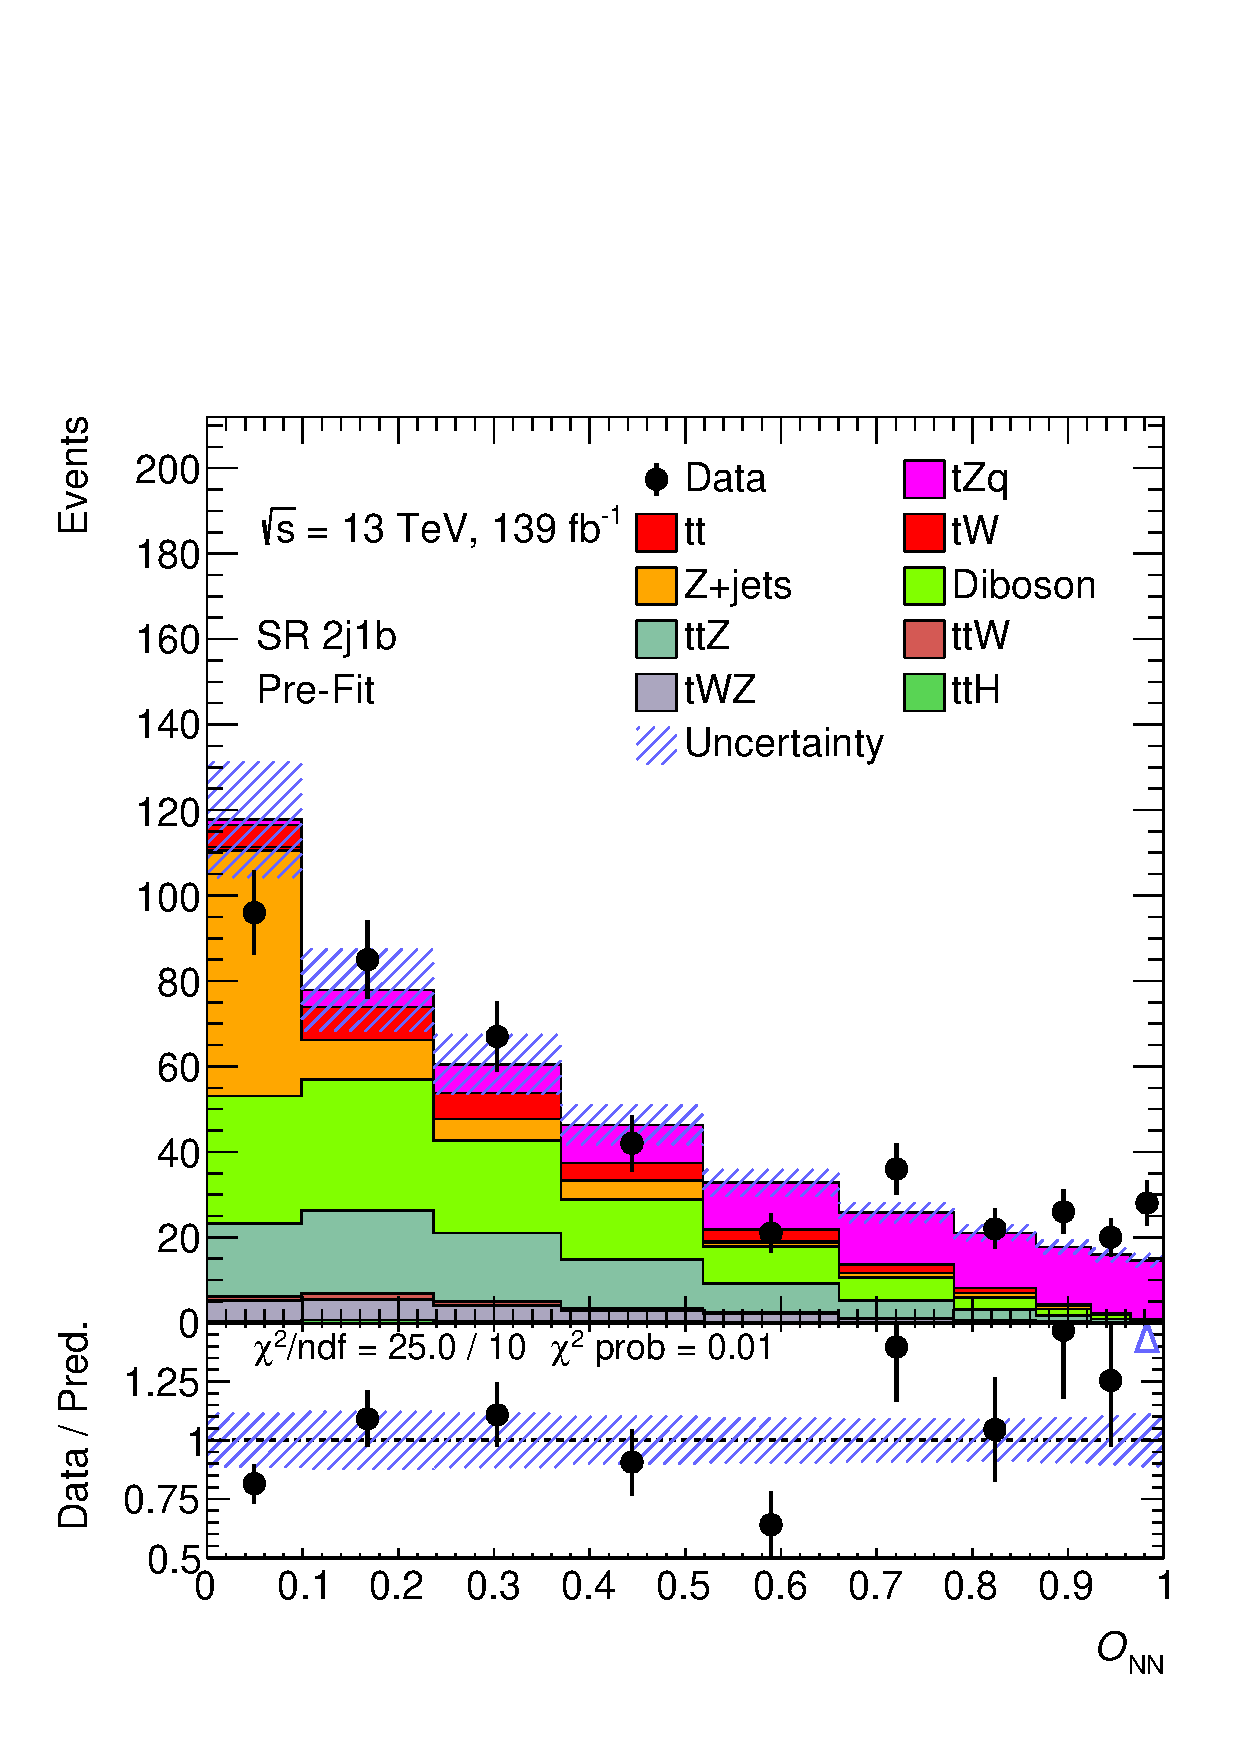
\includegraphics[width=\textwidth]{ubonn-thesis/Chapters/Chapters_07/Figure/Data/SR_2j1b.pdf} 
  \end{subfigure}%% 
  \begin{subfigure}[b]{0.33\linewidth}
    \centering
    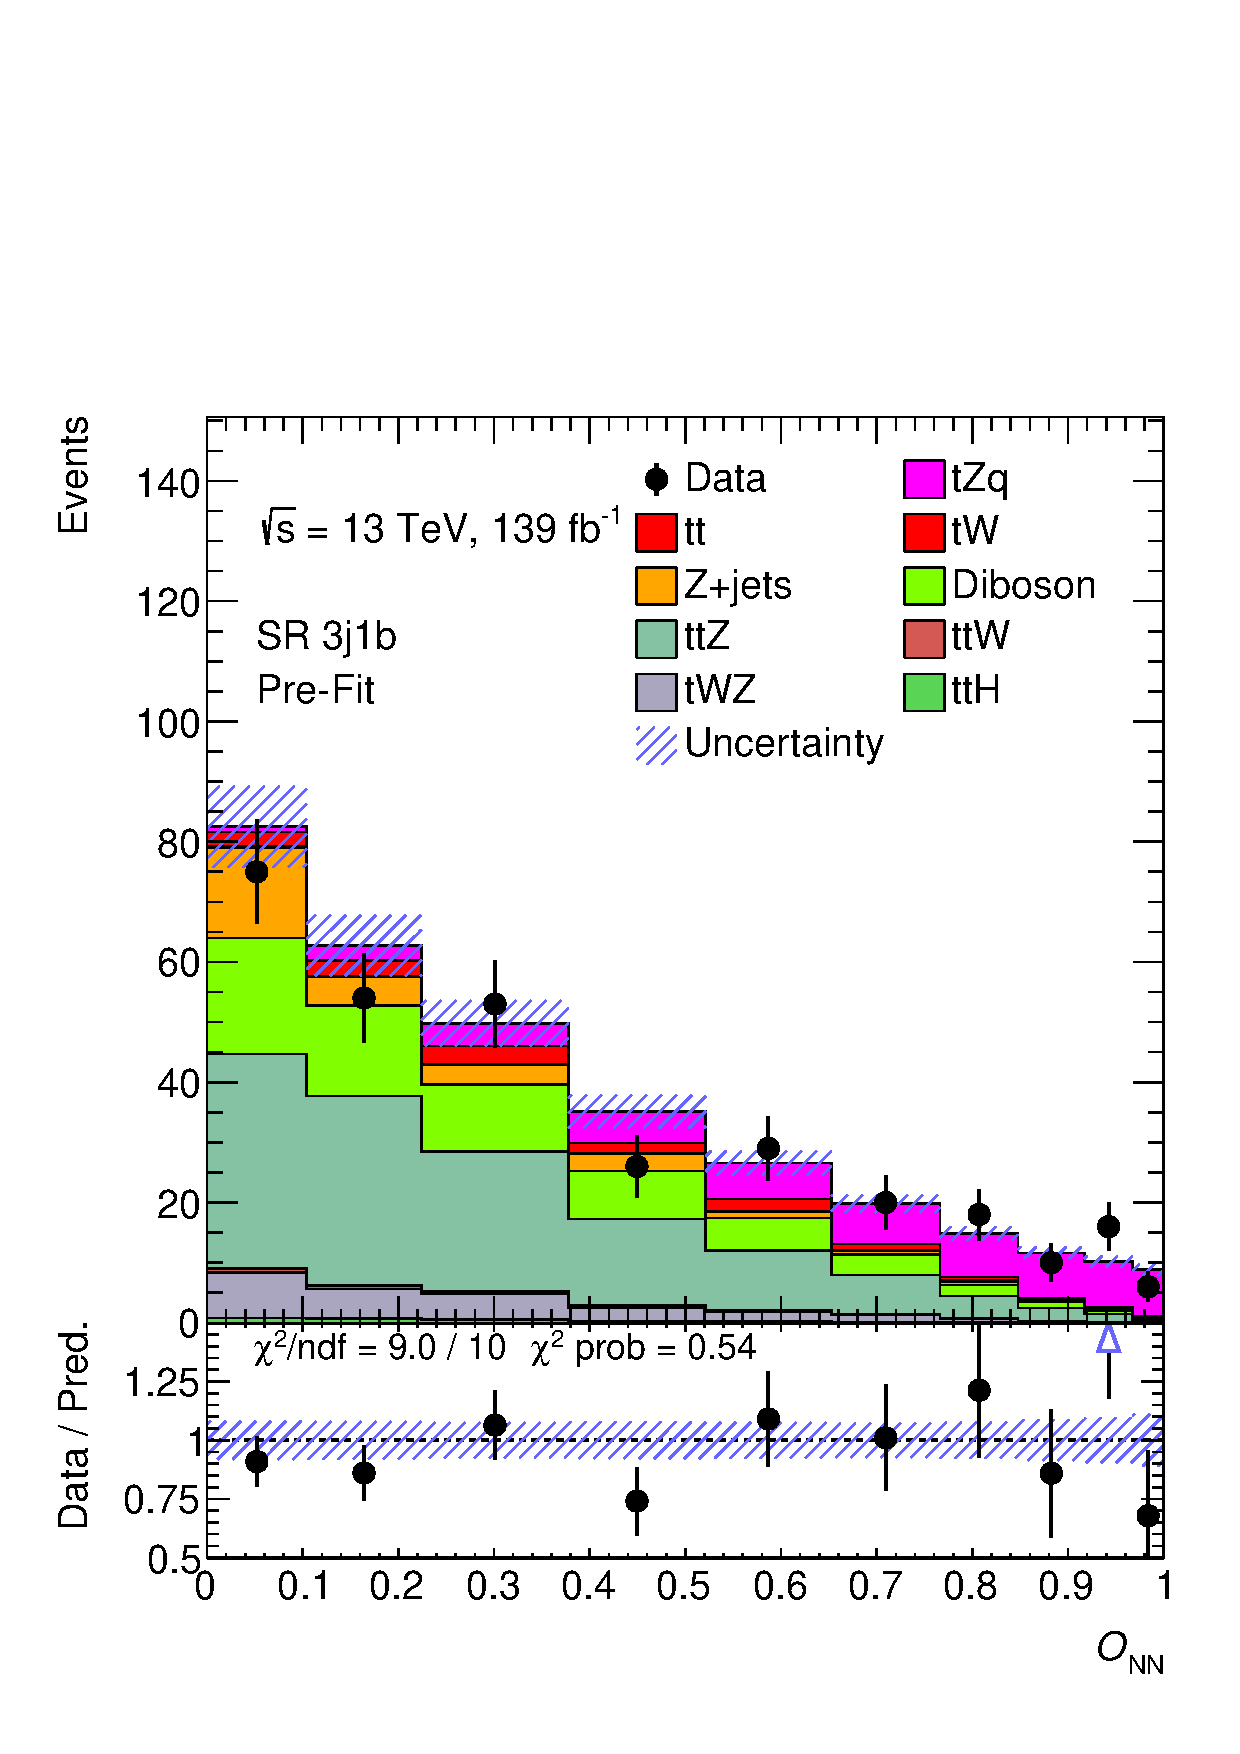
\includegraphics[width=\textwidth]{ubonn-thesis/Chapters/Chapters_07/Figure/Data/SR_3j1b.pdf} 
  \end{subfigure} 
  \begin{subfigure}[b]{0.33\linewidth}
    \centering
    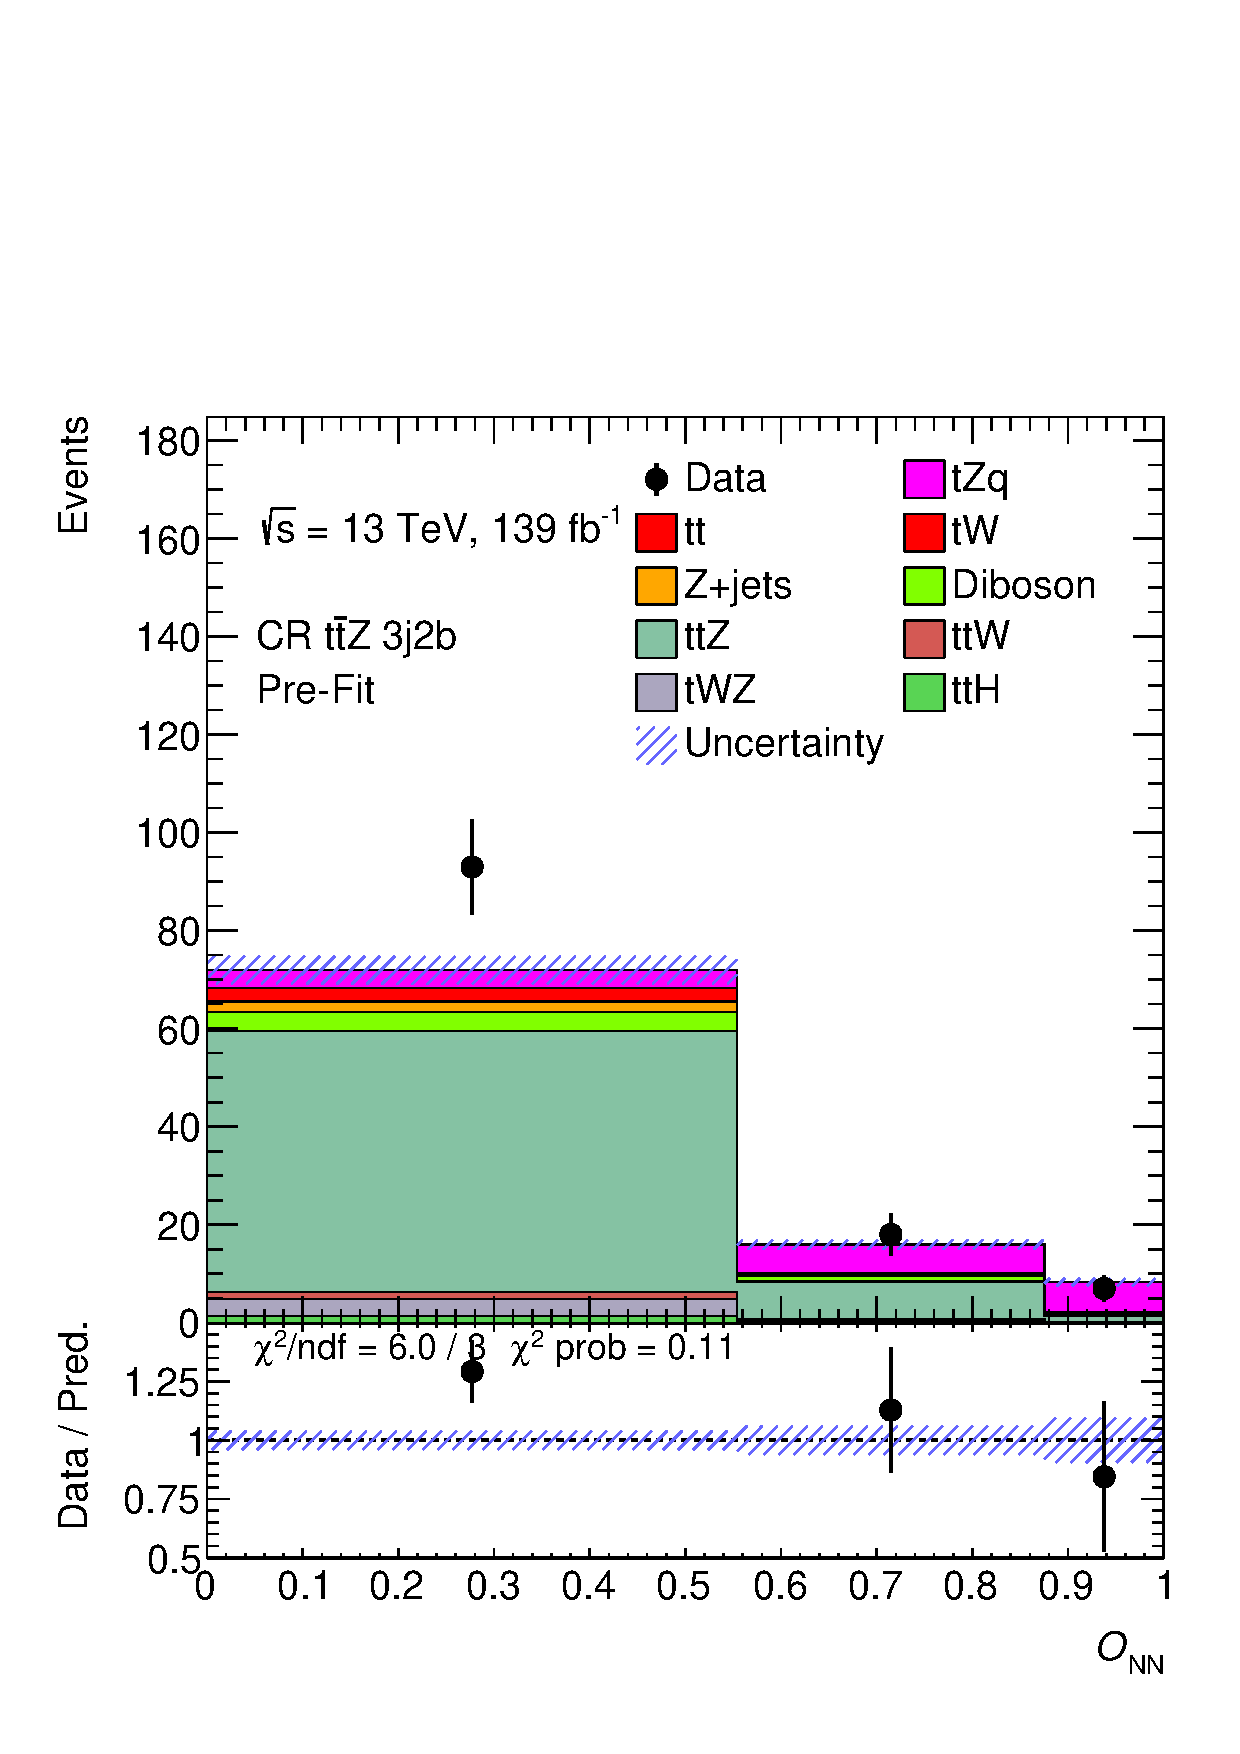
\includegraphics[width=\textwidth]{ubonn-thesis/Chapters/Chapters_07/Figure/Data/CR_3j2b.pdf} 
  \end{subfigure}%%
  \newline
  \begin{subfigure}[b]{0.33\linewidth}
    \centering
    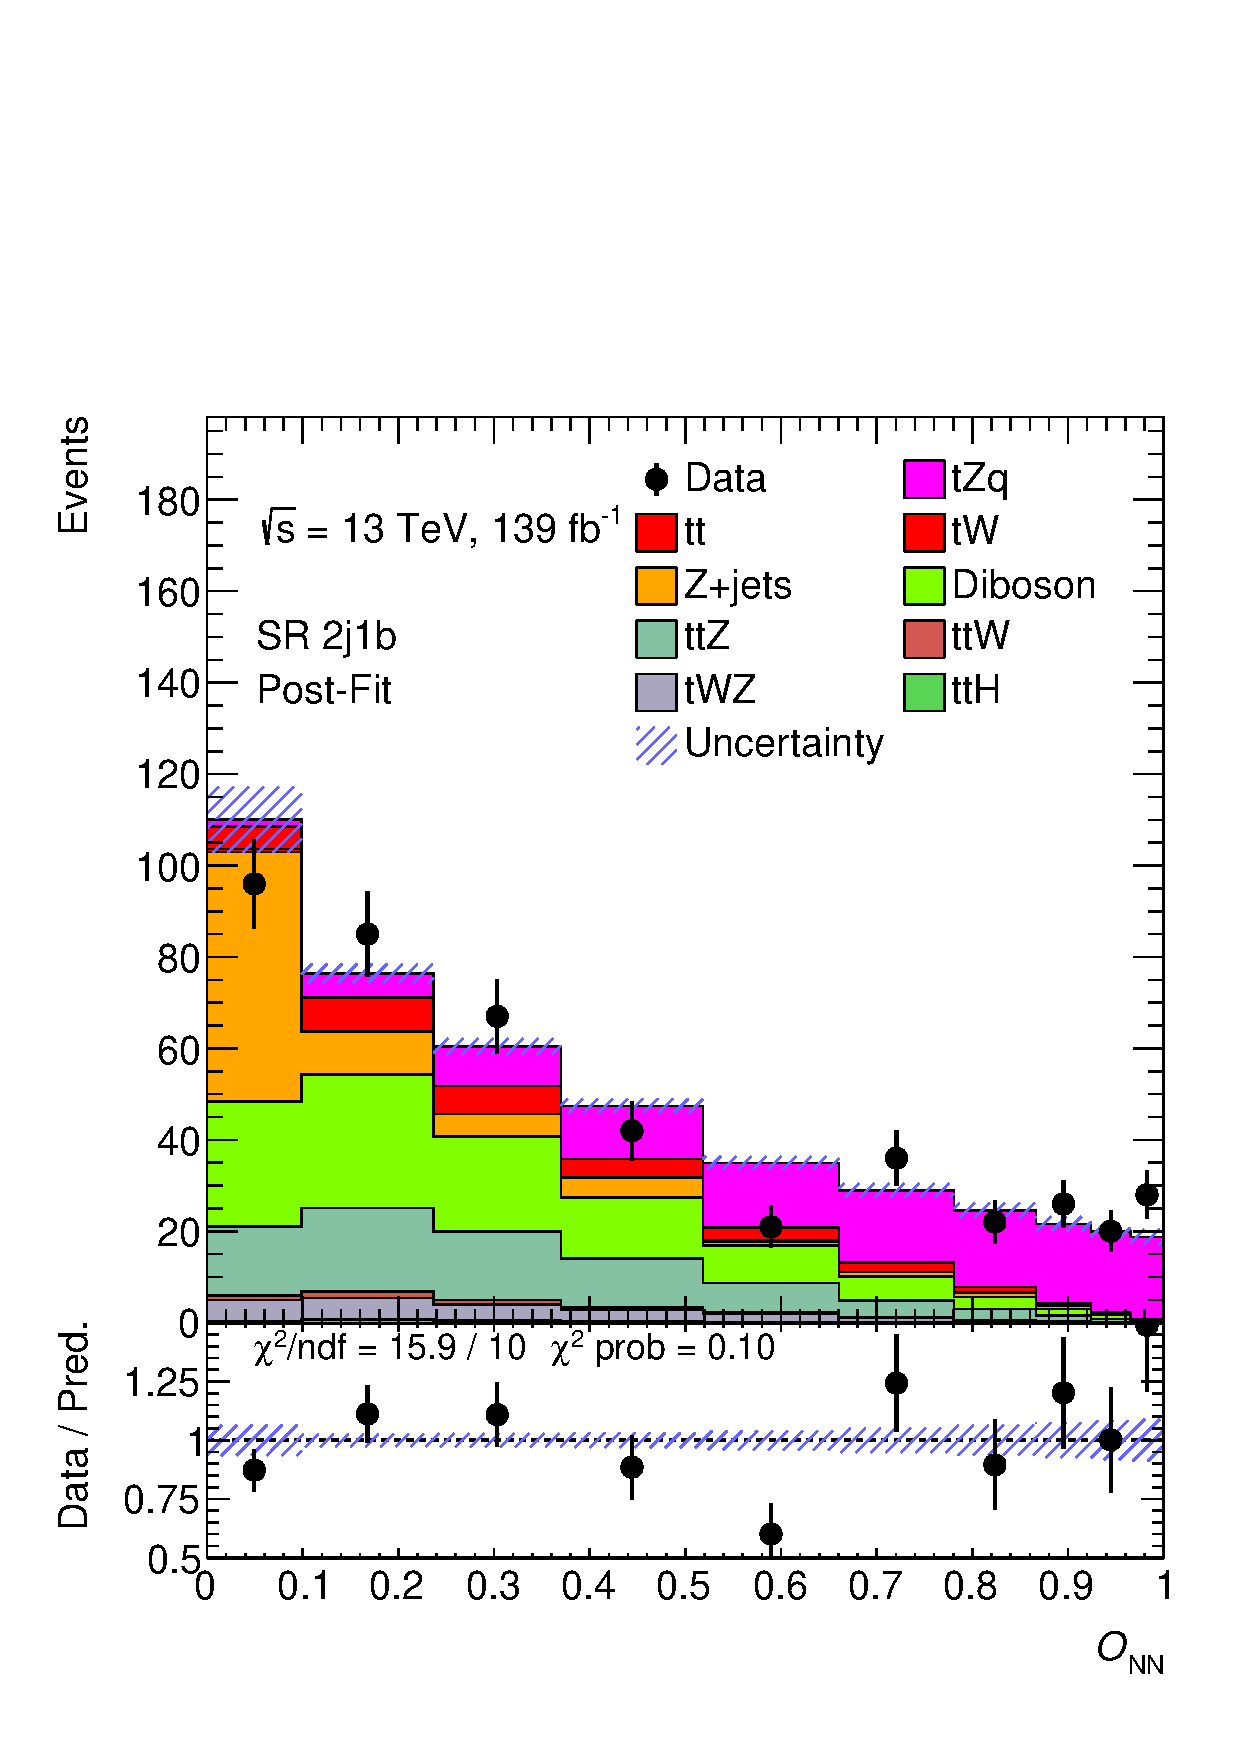
\includegraphics[width=\textwidth]{ubonn-thesis/Chapters/Chapters_07/Figure/Data/SR_2j1b_postFit.pdf} 
  \end{subfigure} 
  \begin{subfigure}[b]{0.33\linewidth}
    \centering
    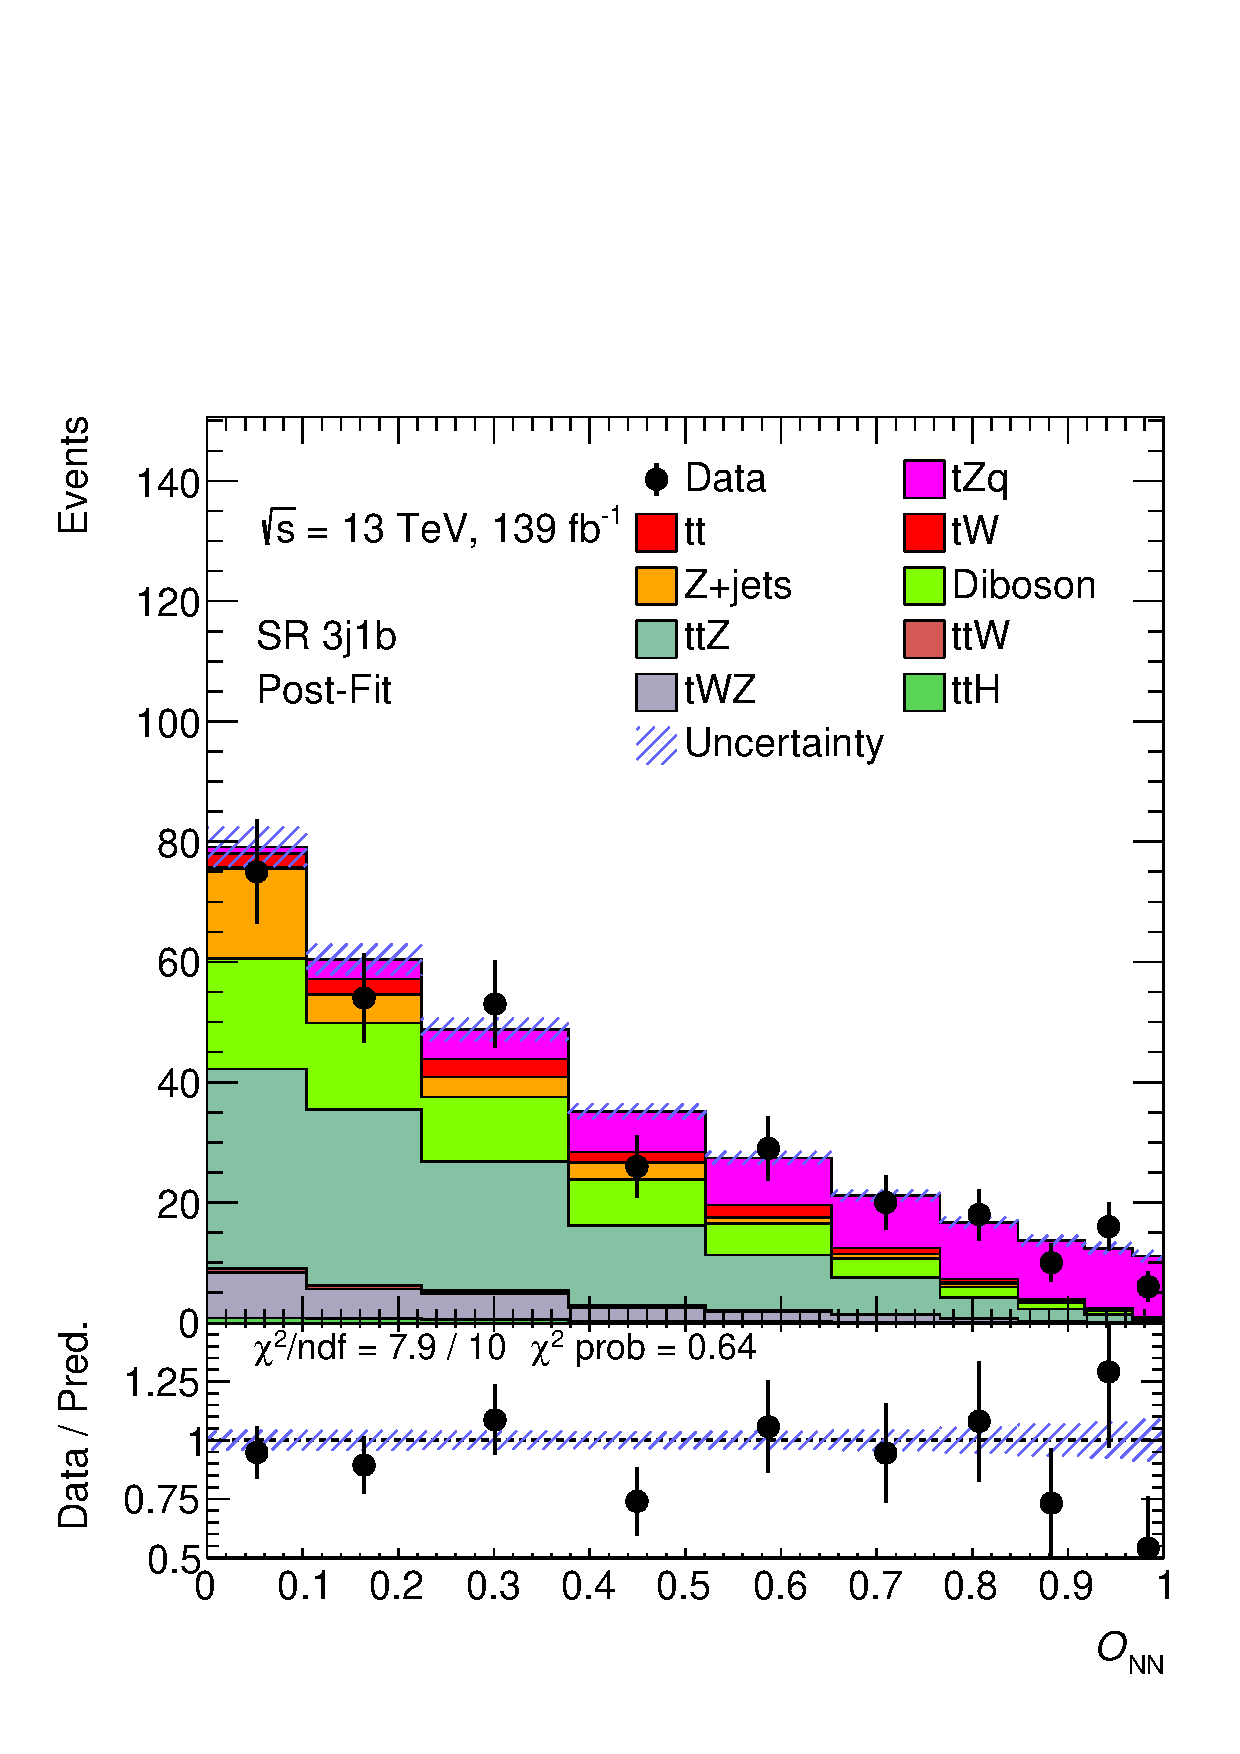
\includegraphics[width=\textwidth]{ubonn-thesis/Chapters/Chapters_07/Figure/Data/SR_3j1b_postFit.pdf} 
  \end{subfigure}%% 
  \begin{subfigure}[b]{0.33\linewidth}
    \centering
    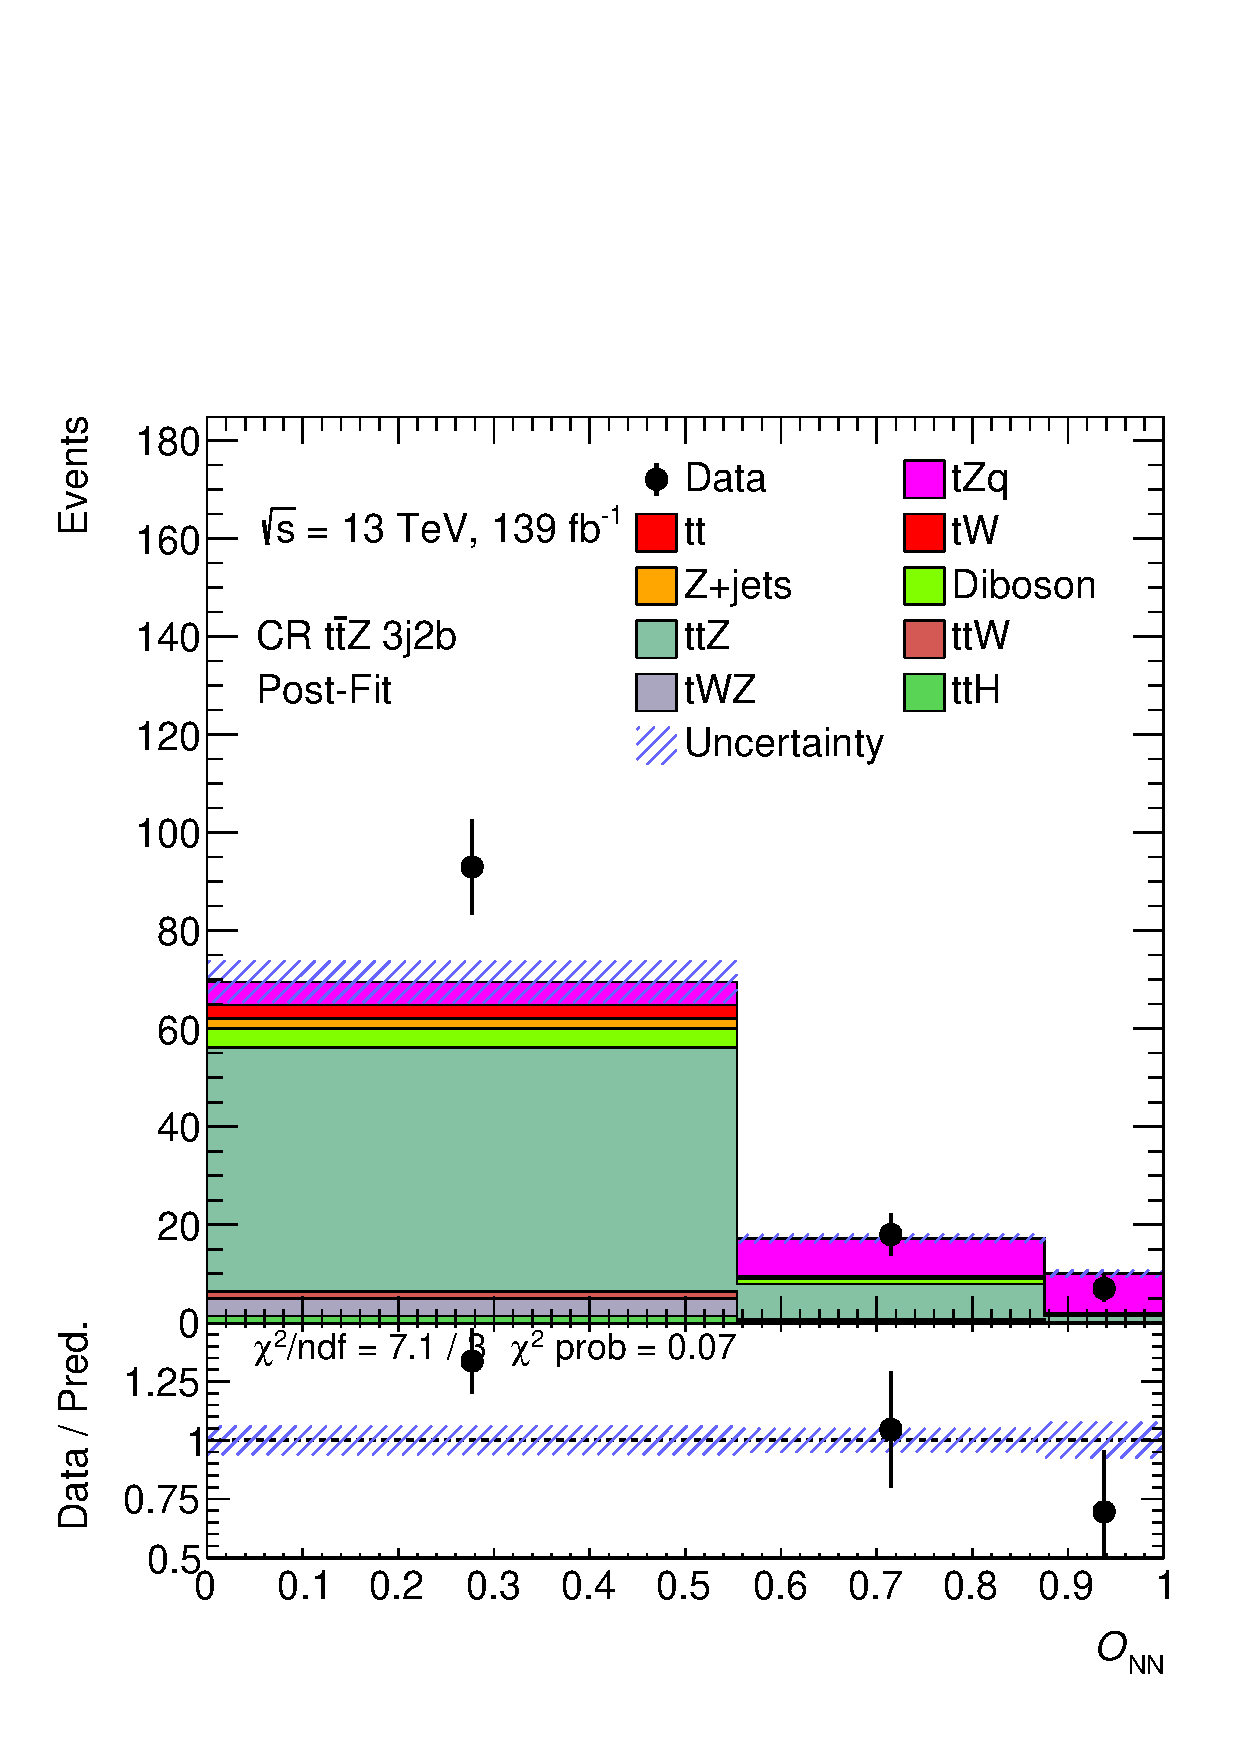
\includegraphics[width=\textwidth]{ubonn-thesis/Chapters/Chapters_07/Figure/Data/CR_3j2b_postFit.pdf} 
  \end{subfigure} 
  \newline
  \begin{subfigure}[b]{0.33\linewidth}
    \centering
    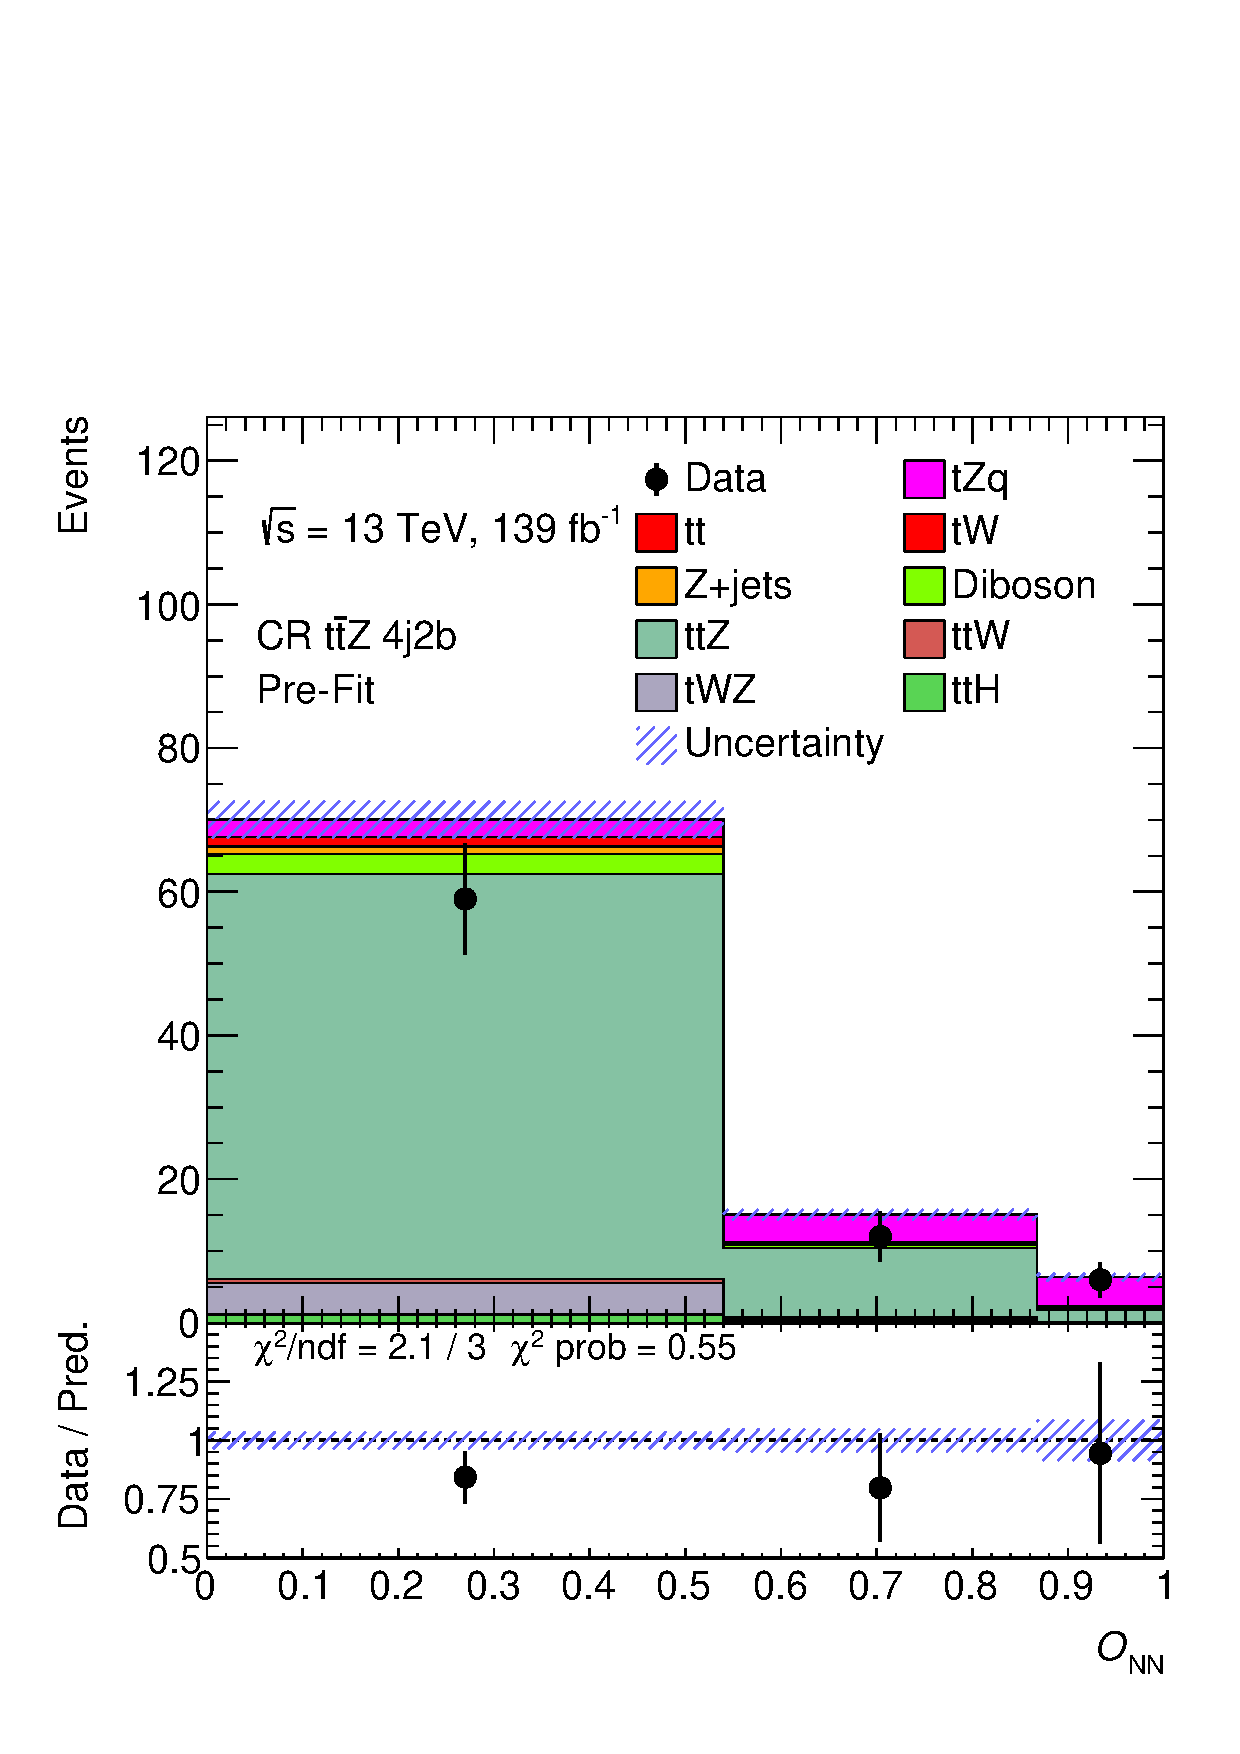
\includegraphics[width=\textwidth]{ubonn-thesis/Chapters/Chapters_07/Figure/Data/CR_4j2b.pdf} 
  \end{subfigure} 
  \begin{subfigure}[b]{0.33\linewidth}
    \centering
    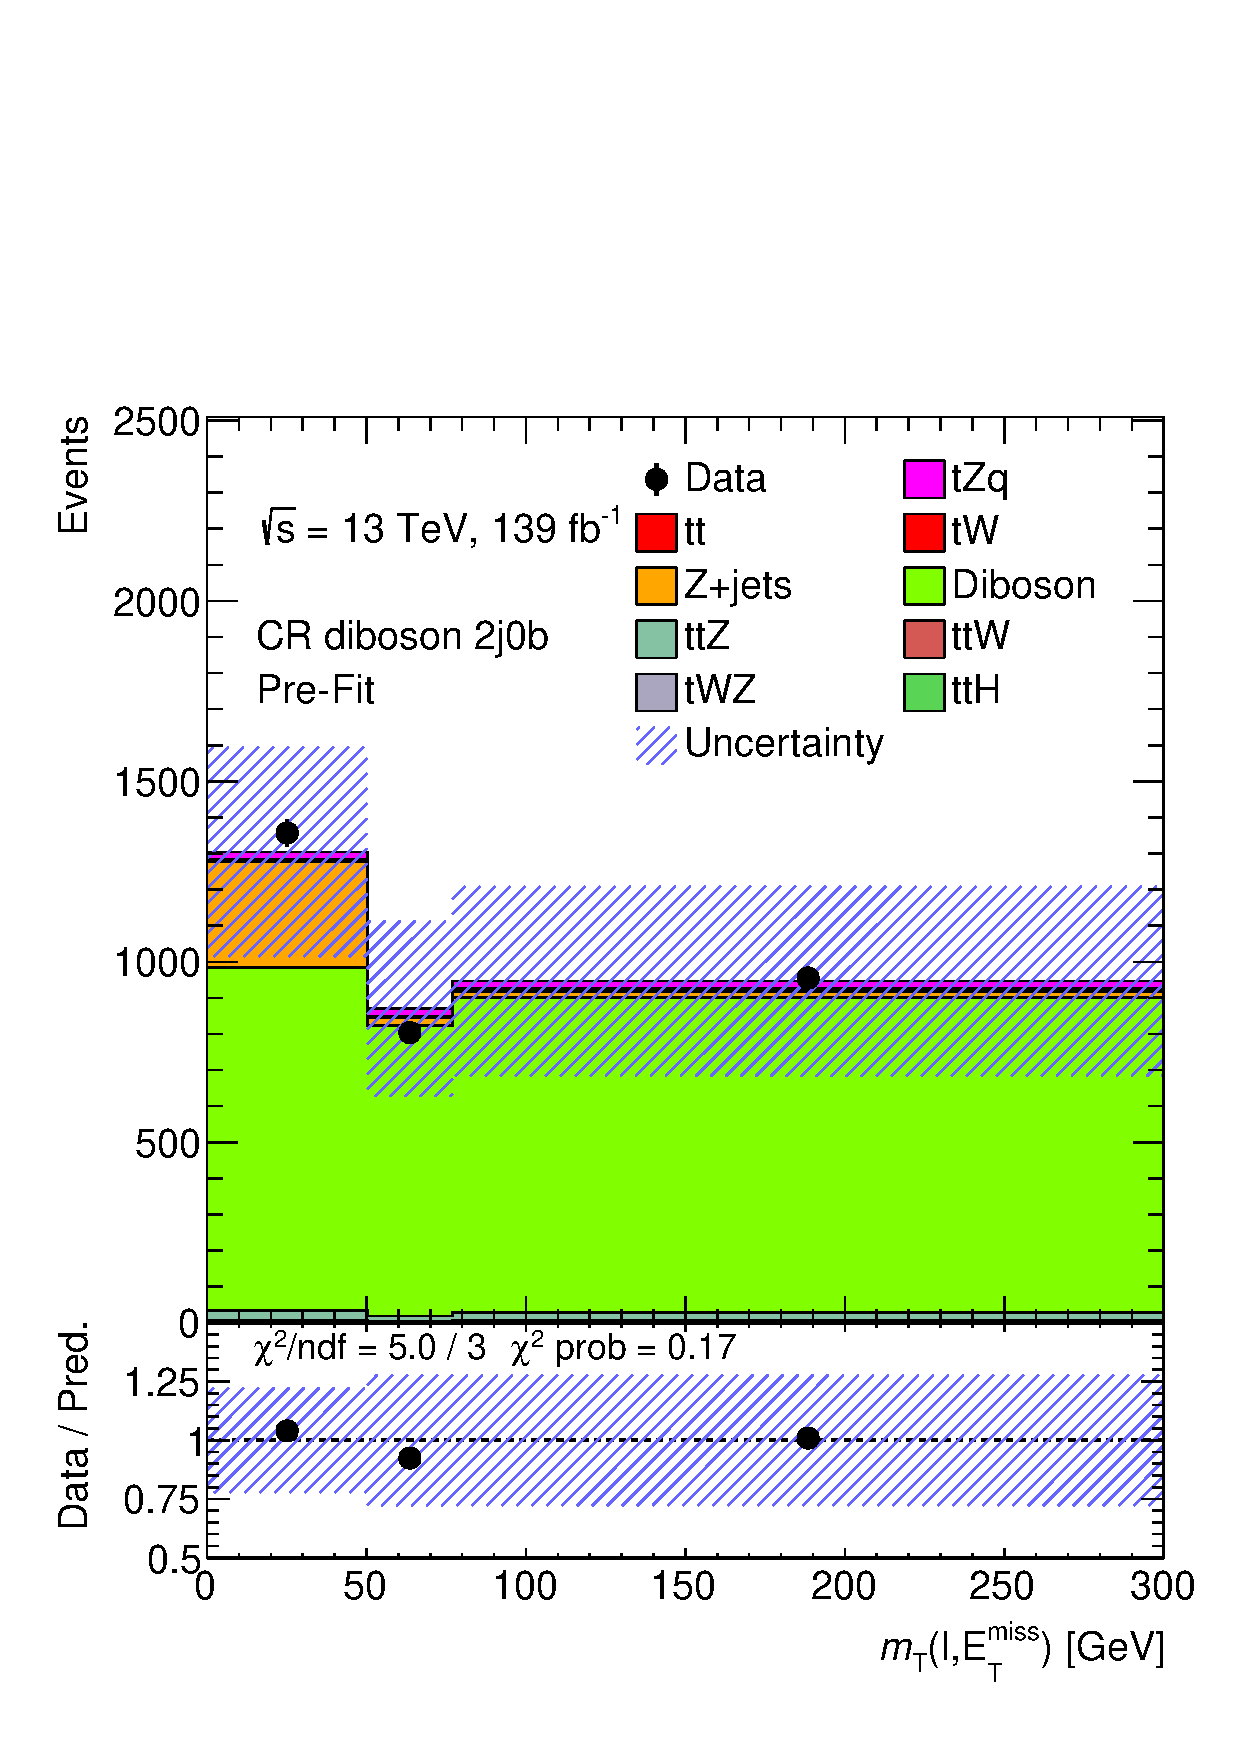
\includegraphics[width=\textwidth]{ubonn-thesis/Chapters/Chapters_07/Figure/Data/CR_2j0b.pdf} 
  \end{subfigure}%% 
  \begin{subfigure}[b]{0.33\linewidth}
    \centering
    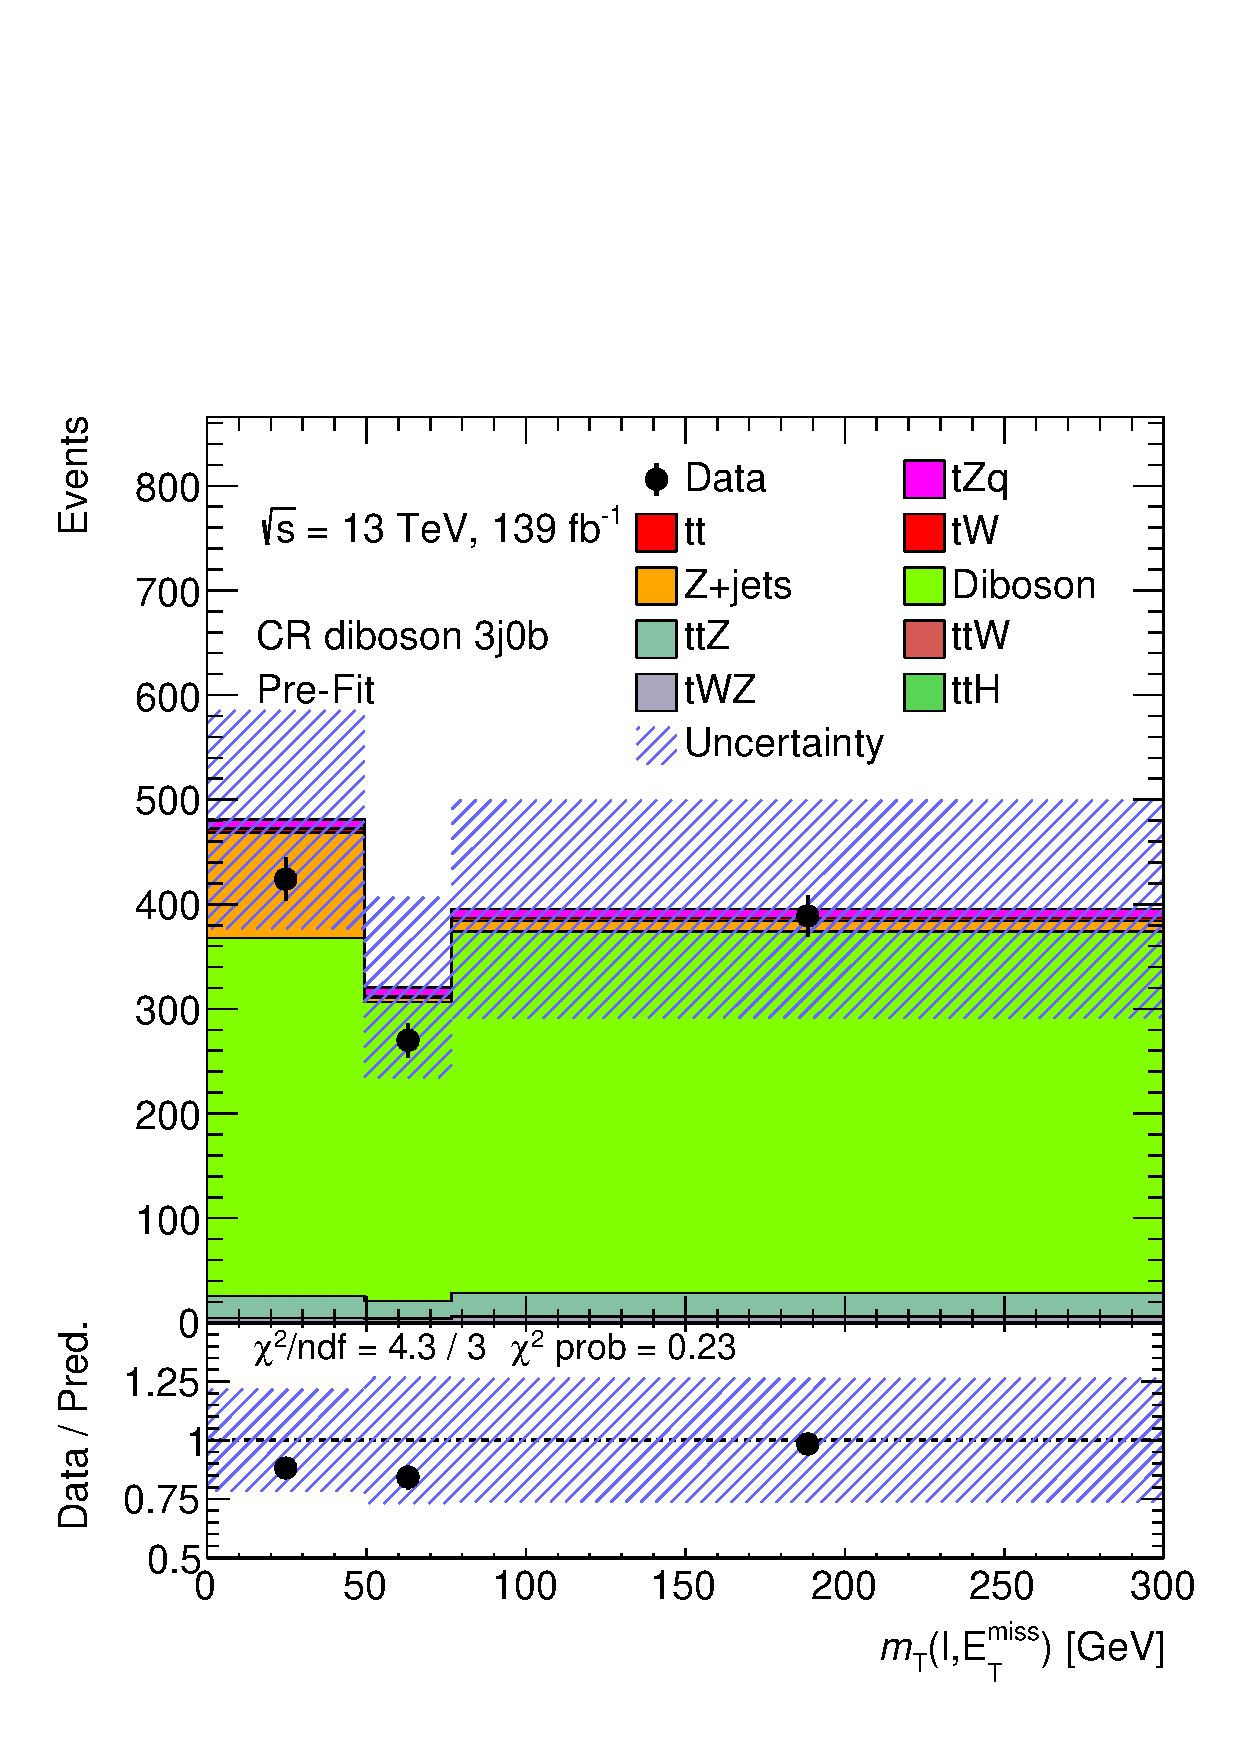
\includegraphics[width=\textwidth]{ubonn-thesis/Chapters/Chapters_07/Figure/Data/CR_3j0b.pdf} 
  \end{subfigure} 
  \caption{ The pre-fit and post-fit distributions in the signal regions and control regions described in the table \ref{tab:fittedregions}. The black points show the unblinded dataset. The error band includes the statistical and systematic uncertainties. $\chi^{2}-$value, number of degree of freedom, and corresponding p-vale of $\chi^{2}$ fit are shown in Data/Pred. ratio  plot.}
  \label{fig:datafit1}
\end{figure}

\begin{figure}[!h] 
  \begin{subfigure}[b]{0.33\linewidth}
    \centering
    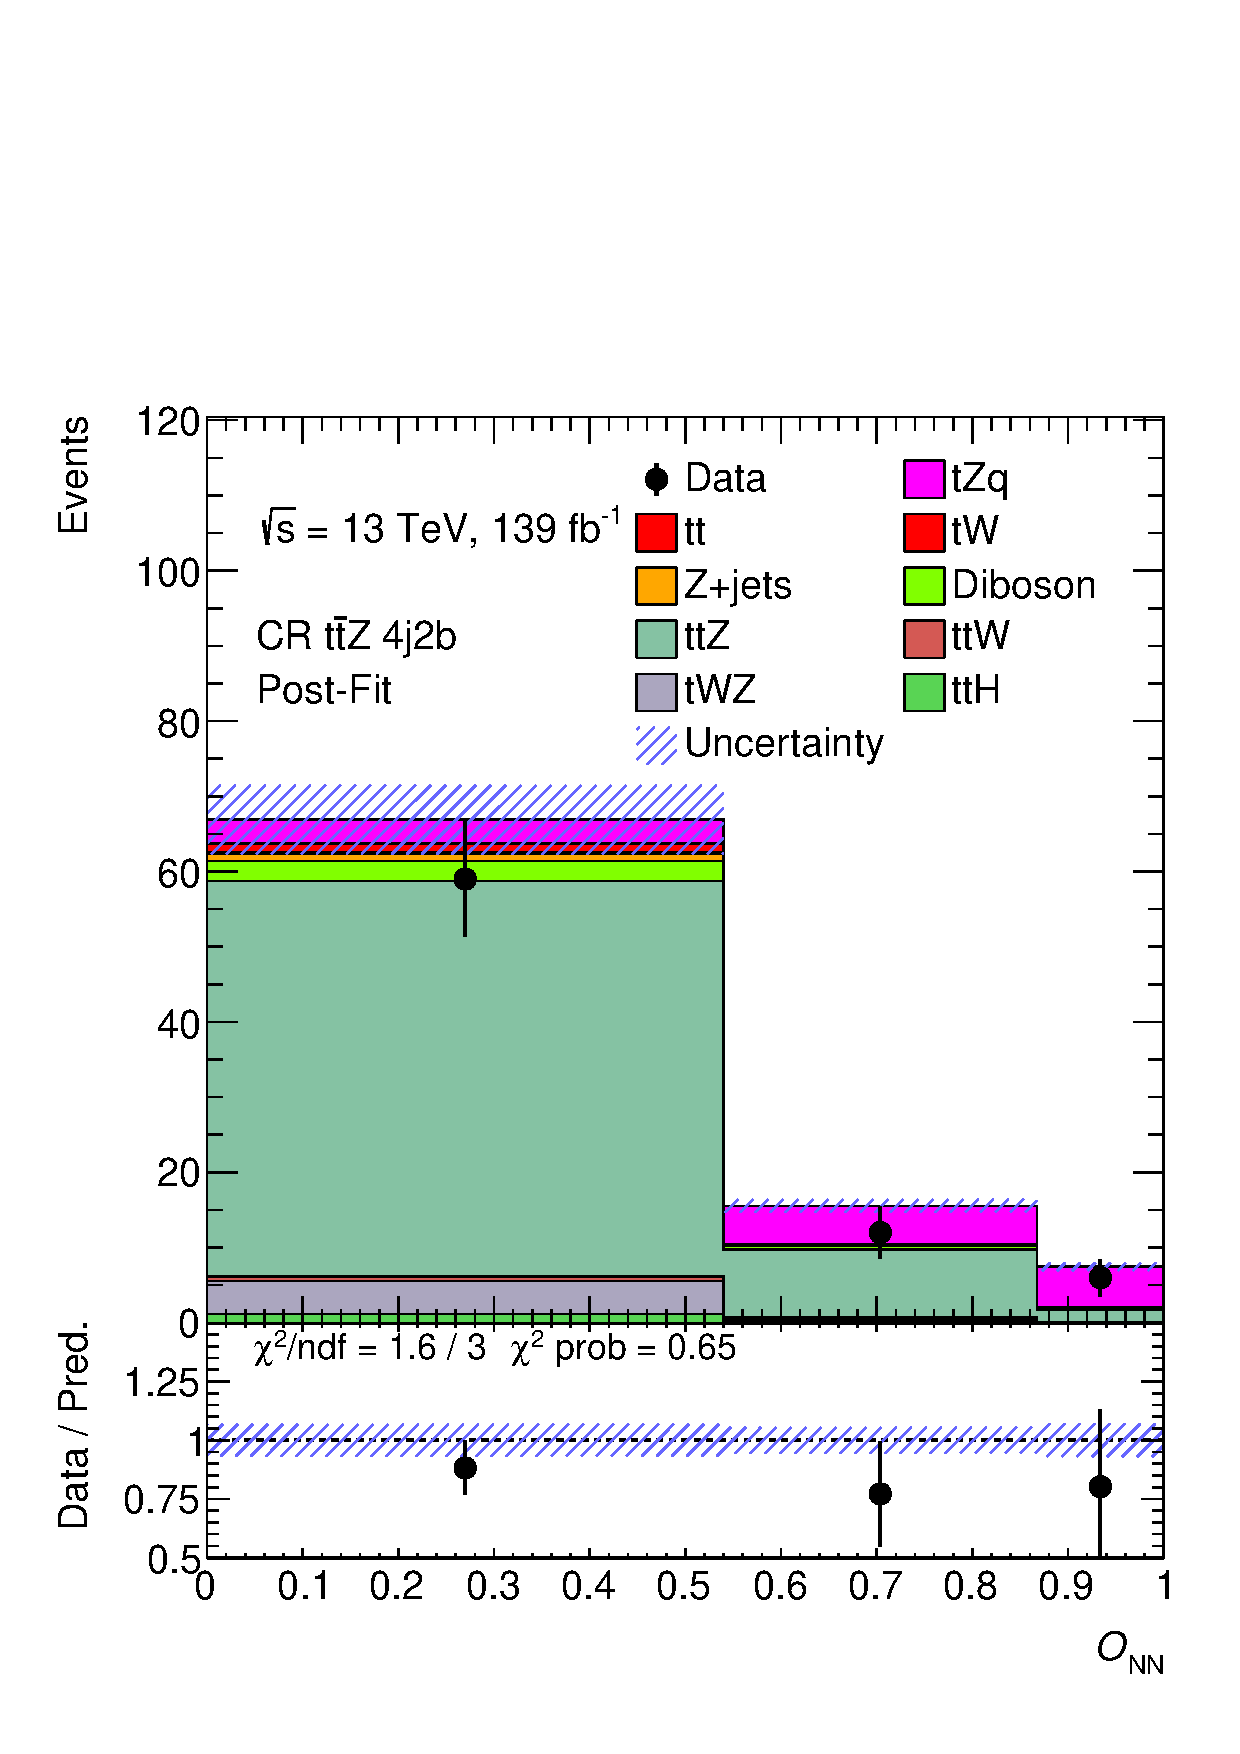
\includegraphics[width=\textwidth]{ubonn-thesis/Chapters/Chapters_07/Figure/Data/CR_4j2b_postFit.pdf} 
    \caption{}
  \end{subfigure}%% 
  \begin{subfigure}[b]{0.33\linewidth}
    \centering
    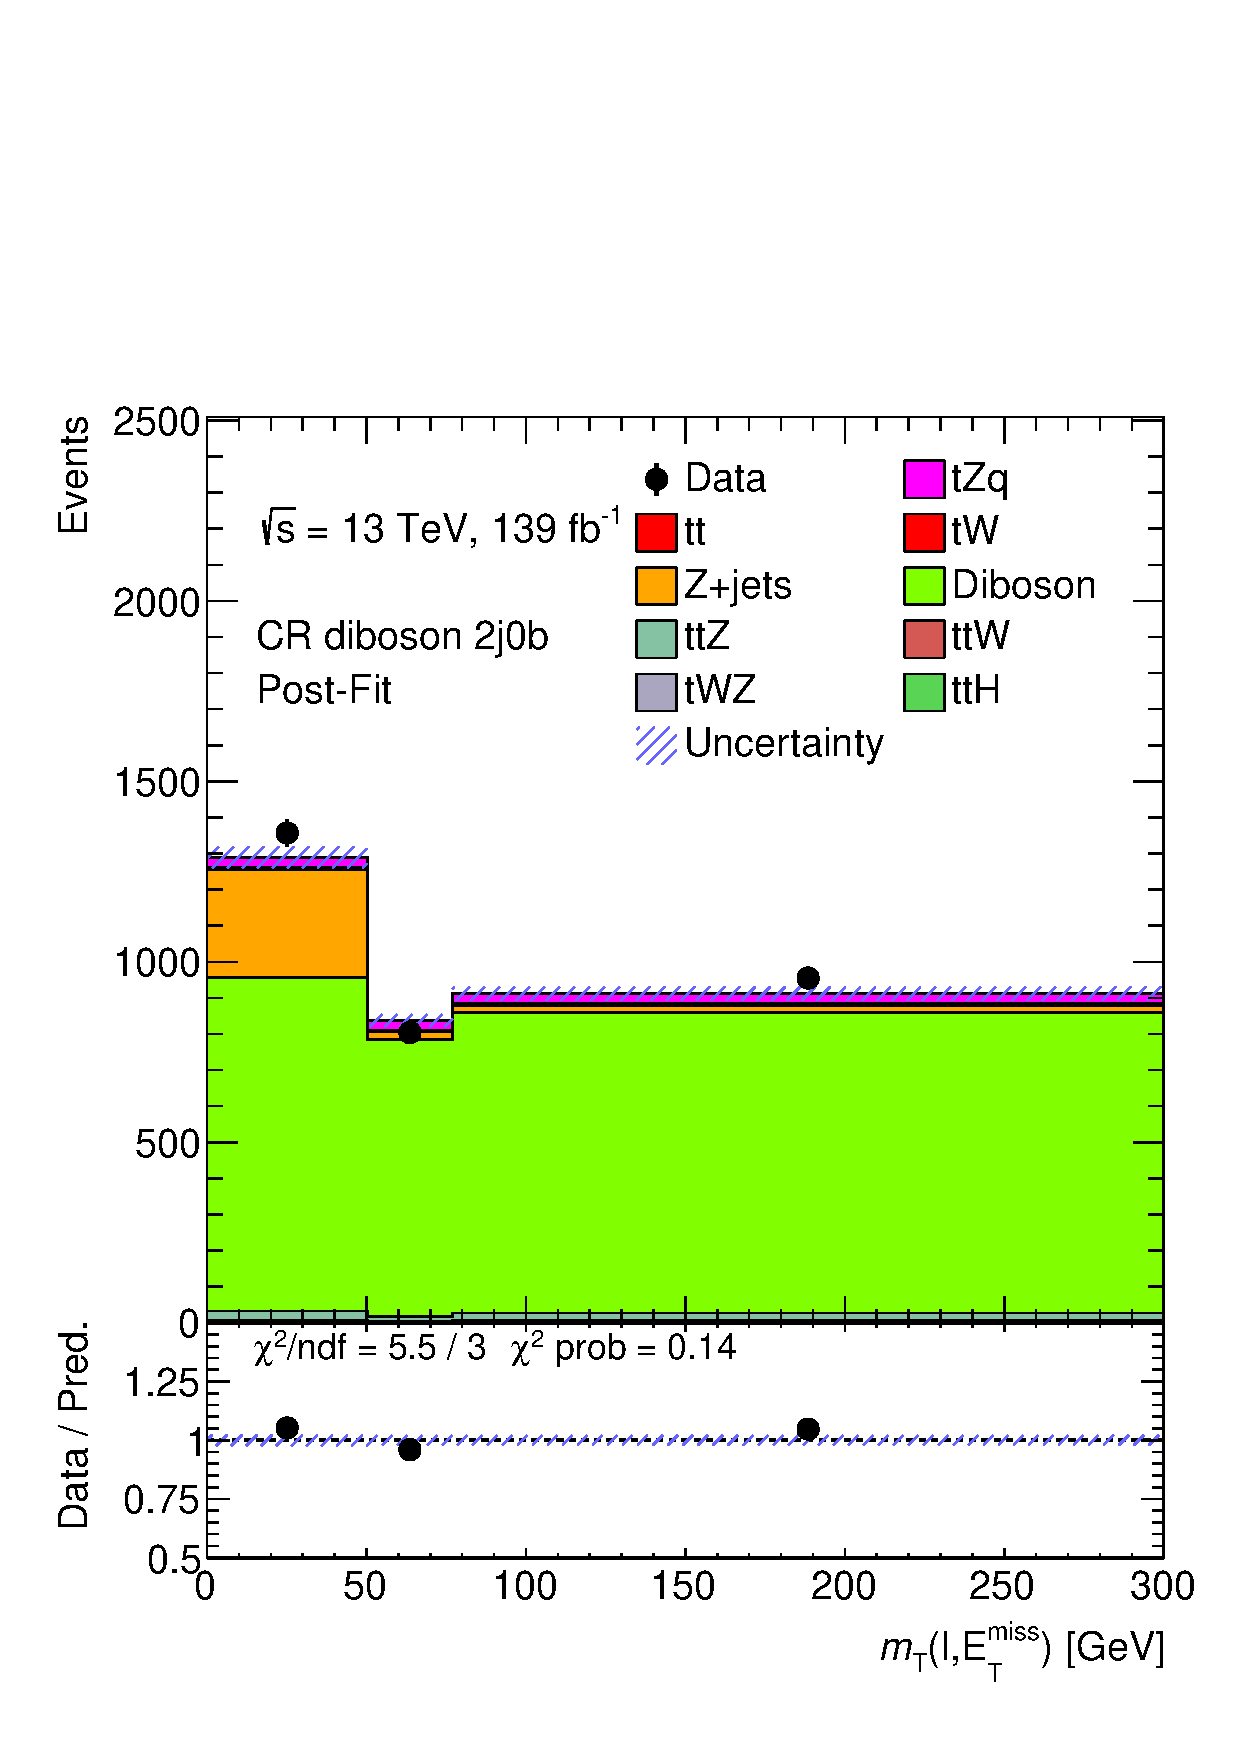
\includegraphics[width=\textwidth]{ubonn-thesis/Chapters/Chapters_07/Figure/Data/CR_2j0b_postFit.pdf} 
    \caption{}
  \end{subfigure} 
  \begin{subfigure}[b]{0.33\linewidth}
    \centering
    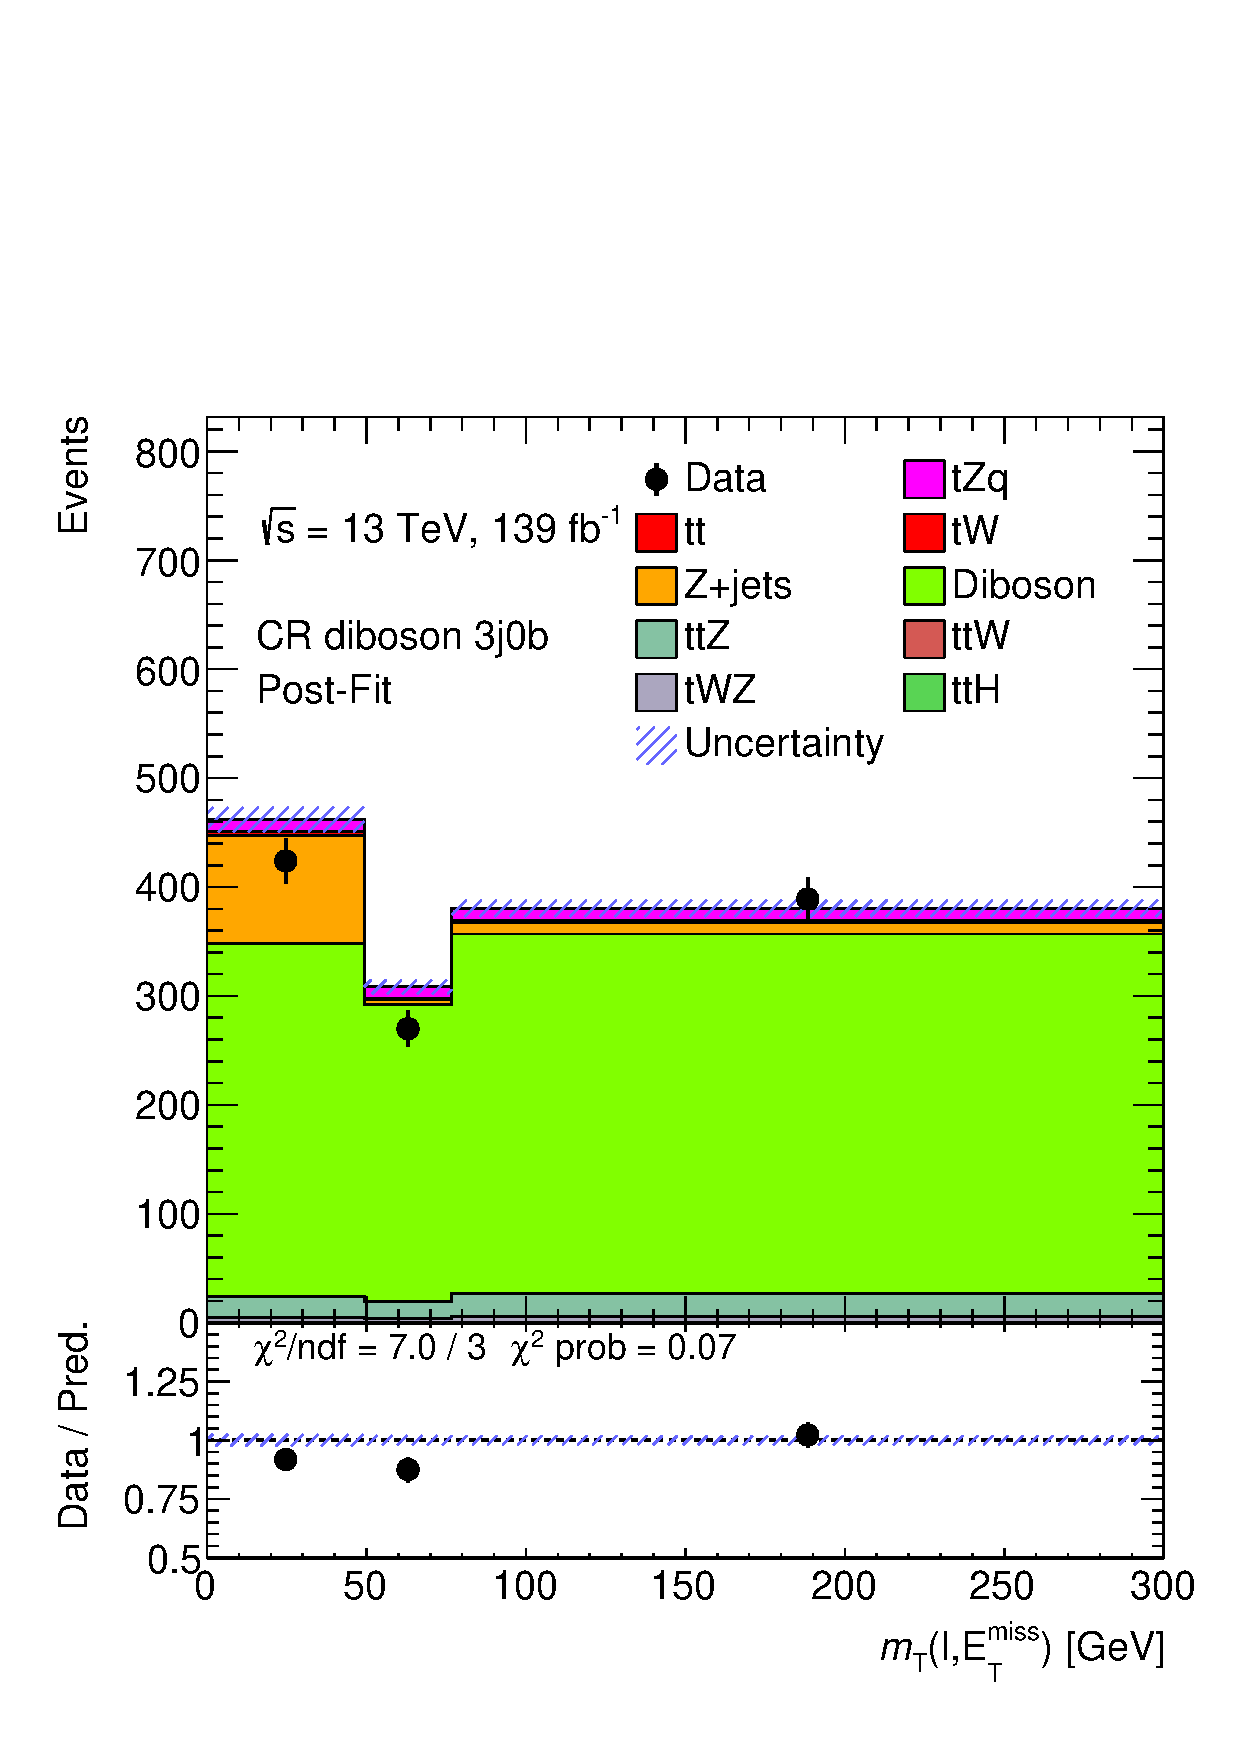
\includegraphics[width=\textwidth]{ubonn-thesis/Chapters/Chapters_07/Figure/Data/CR_3j0b_postFit.pdf} 
    \caption{}
  \end{subfigure}%%
  \newline
  \centering
  \begin{subfigure}[b]{0.33\linewidth}
    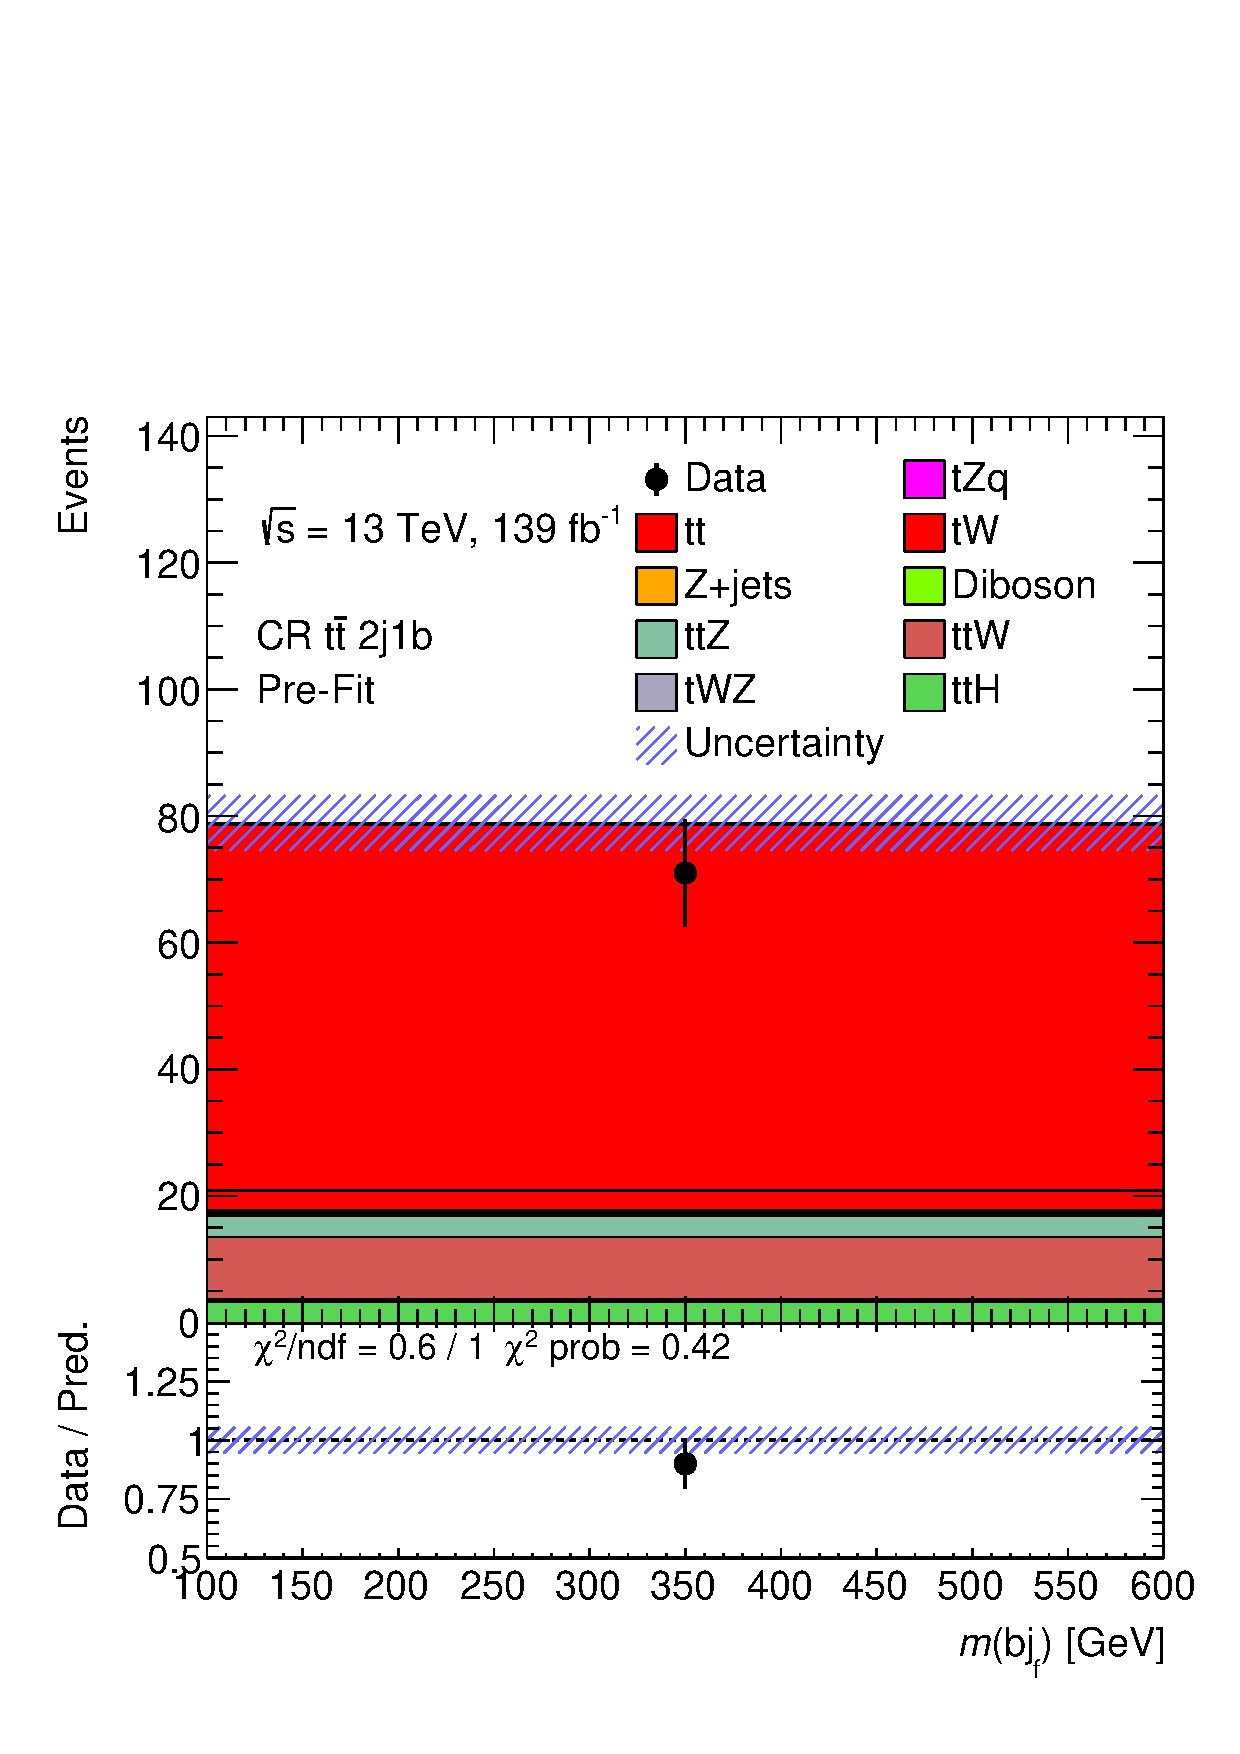
\includegraphics[width=\textwidth]{ubonn-thesis/Chapters/Chapters_07/Figure/Data/CR_2j1b.pdf} 
    \caption{}
  \end{subfigure} 
  \centering
  \begin{subfigure}[b]{0.33\linewidth}
    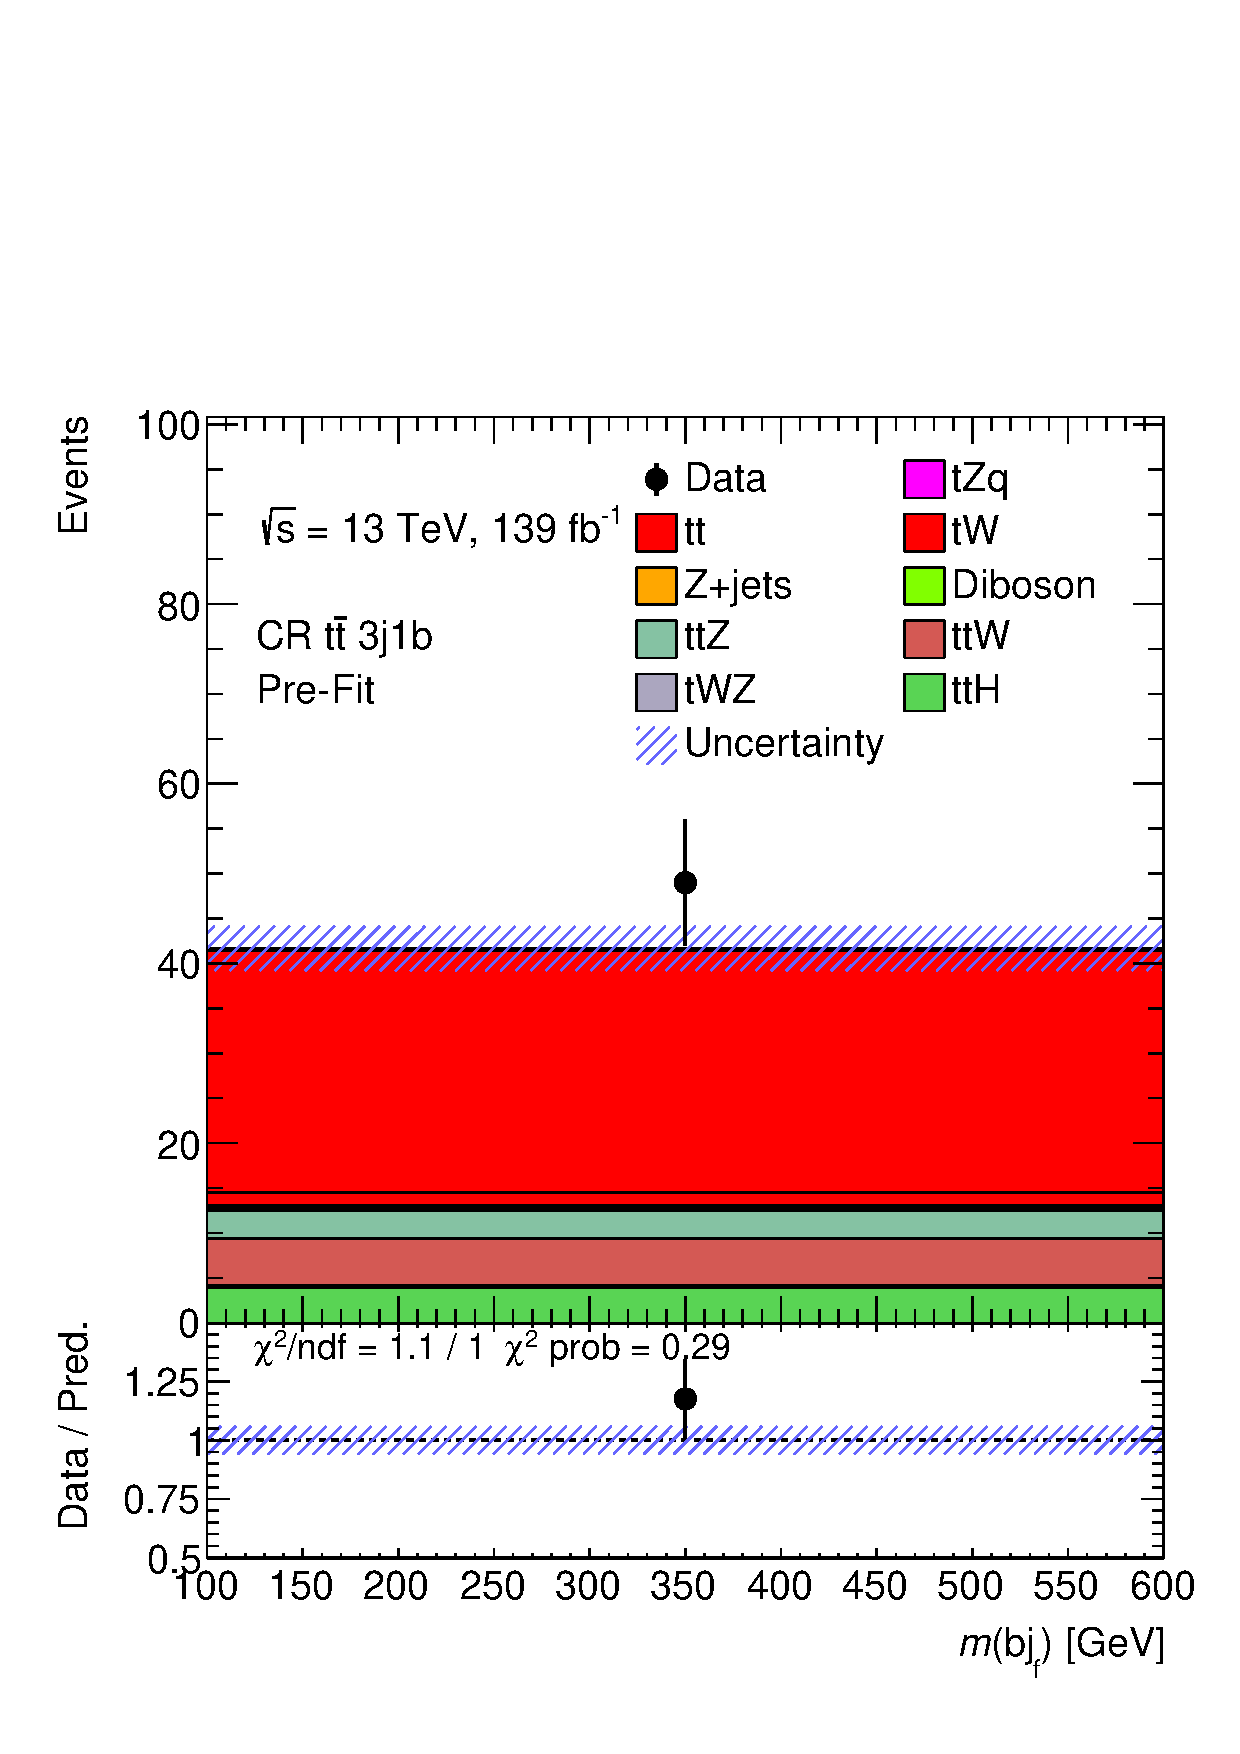
\includegraphics[width=\textwidth]{ubonn-thesis/Chapters/Chapters_07/Figure/Data/CR_3j1b.pdf} 
    \caption{}
  \end{subfigure}%% 
  \newline
  \hspace*{-1.5cm}
  \begin{subfigure}[b]{0.33\linewidth}
   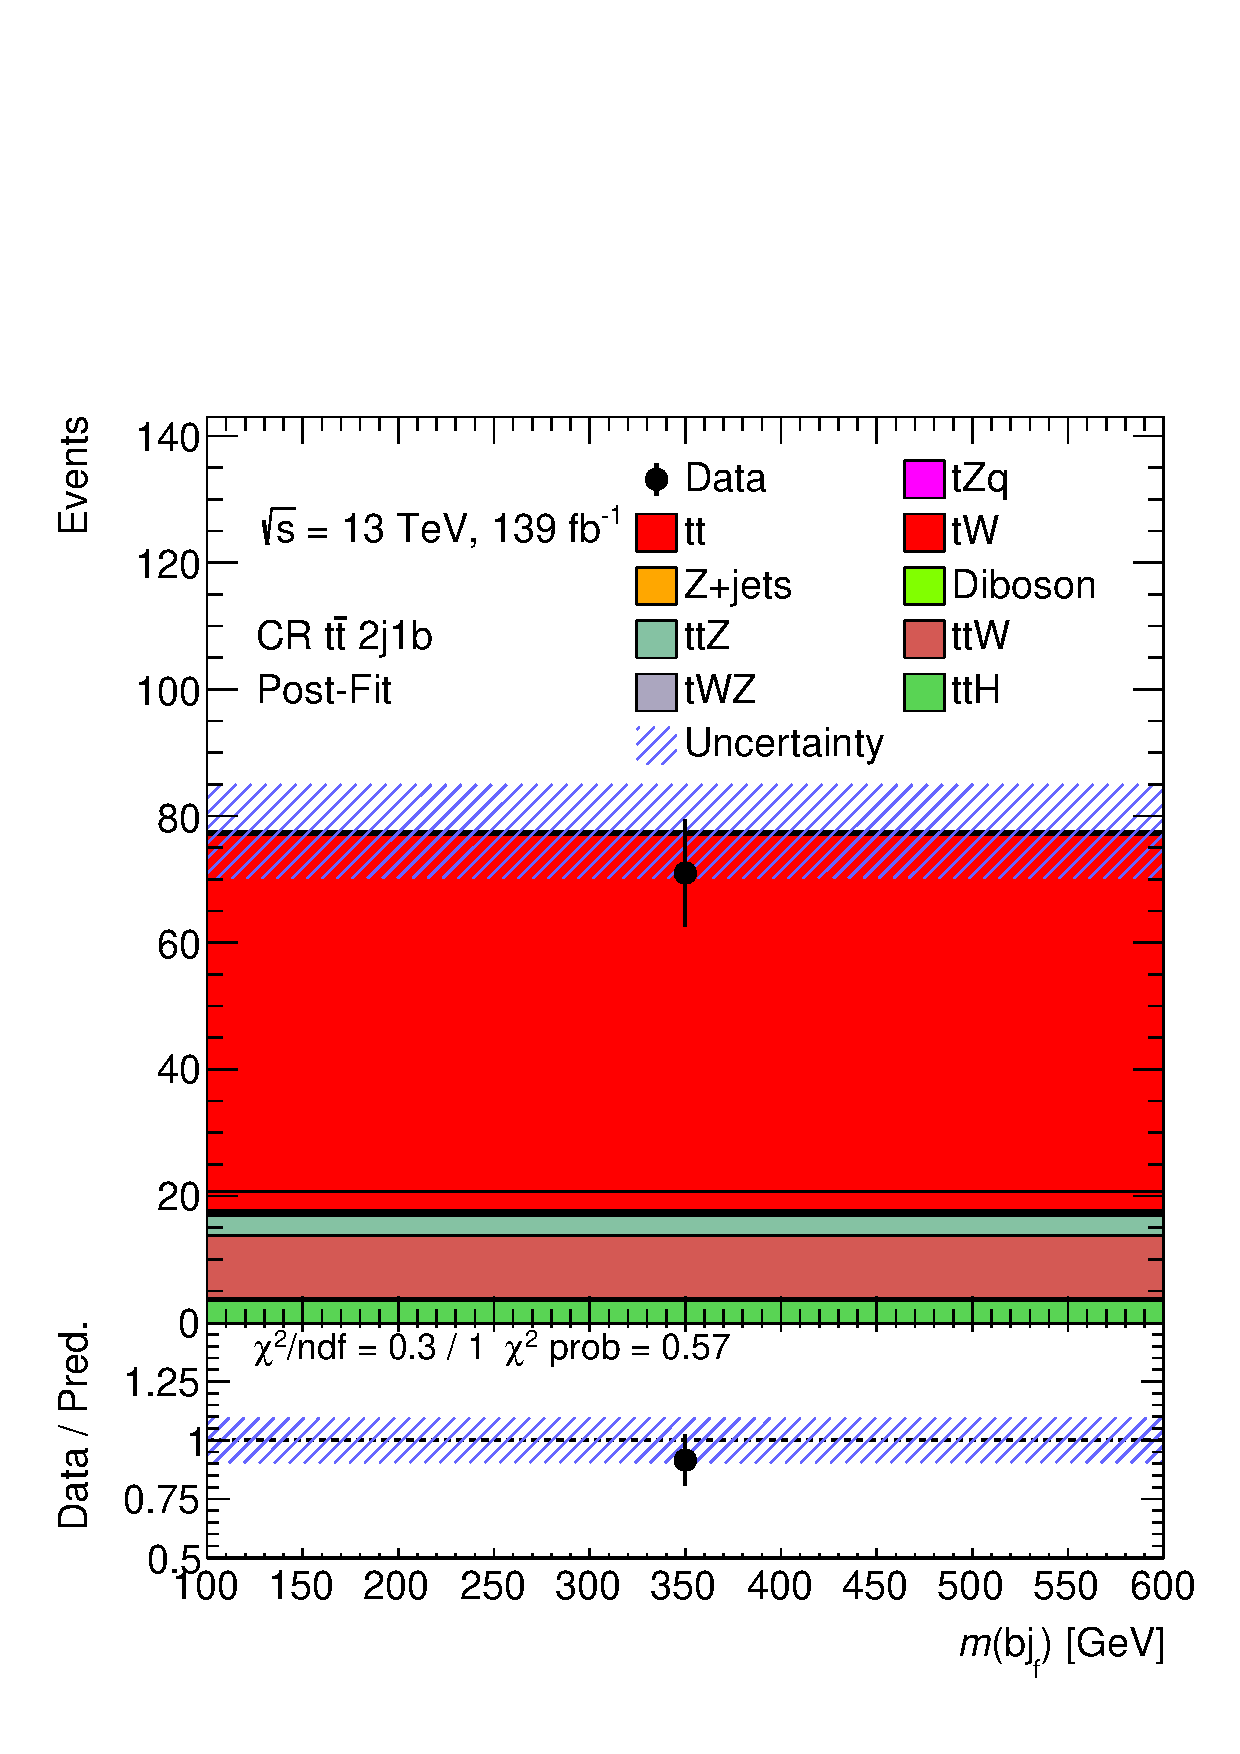
\includegraphics[width=\textwidth]{ubonn-thesis/Chapters/Chapters_07/Figure/Data/CR_2j1b_postFit.pdf} 
    \caption{}
  \end{subfigure} 
  \centering
  \begin{subfigure}[b]{0.33\linewidth}
  %\hspace*{-1.0cm}
    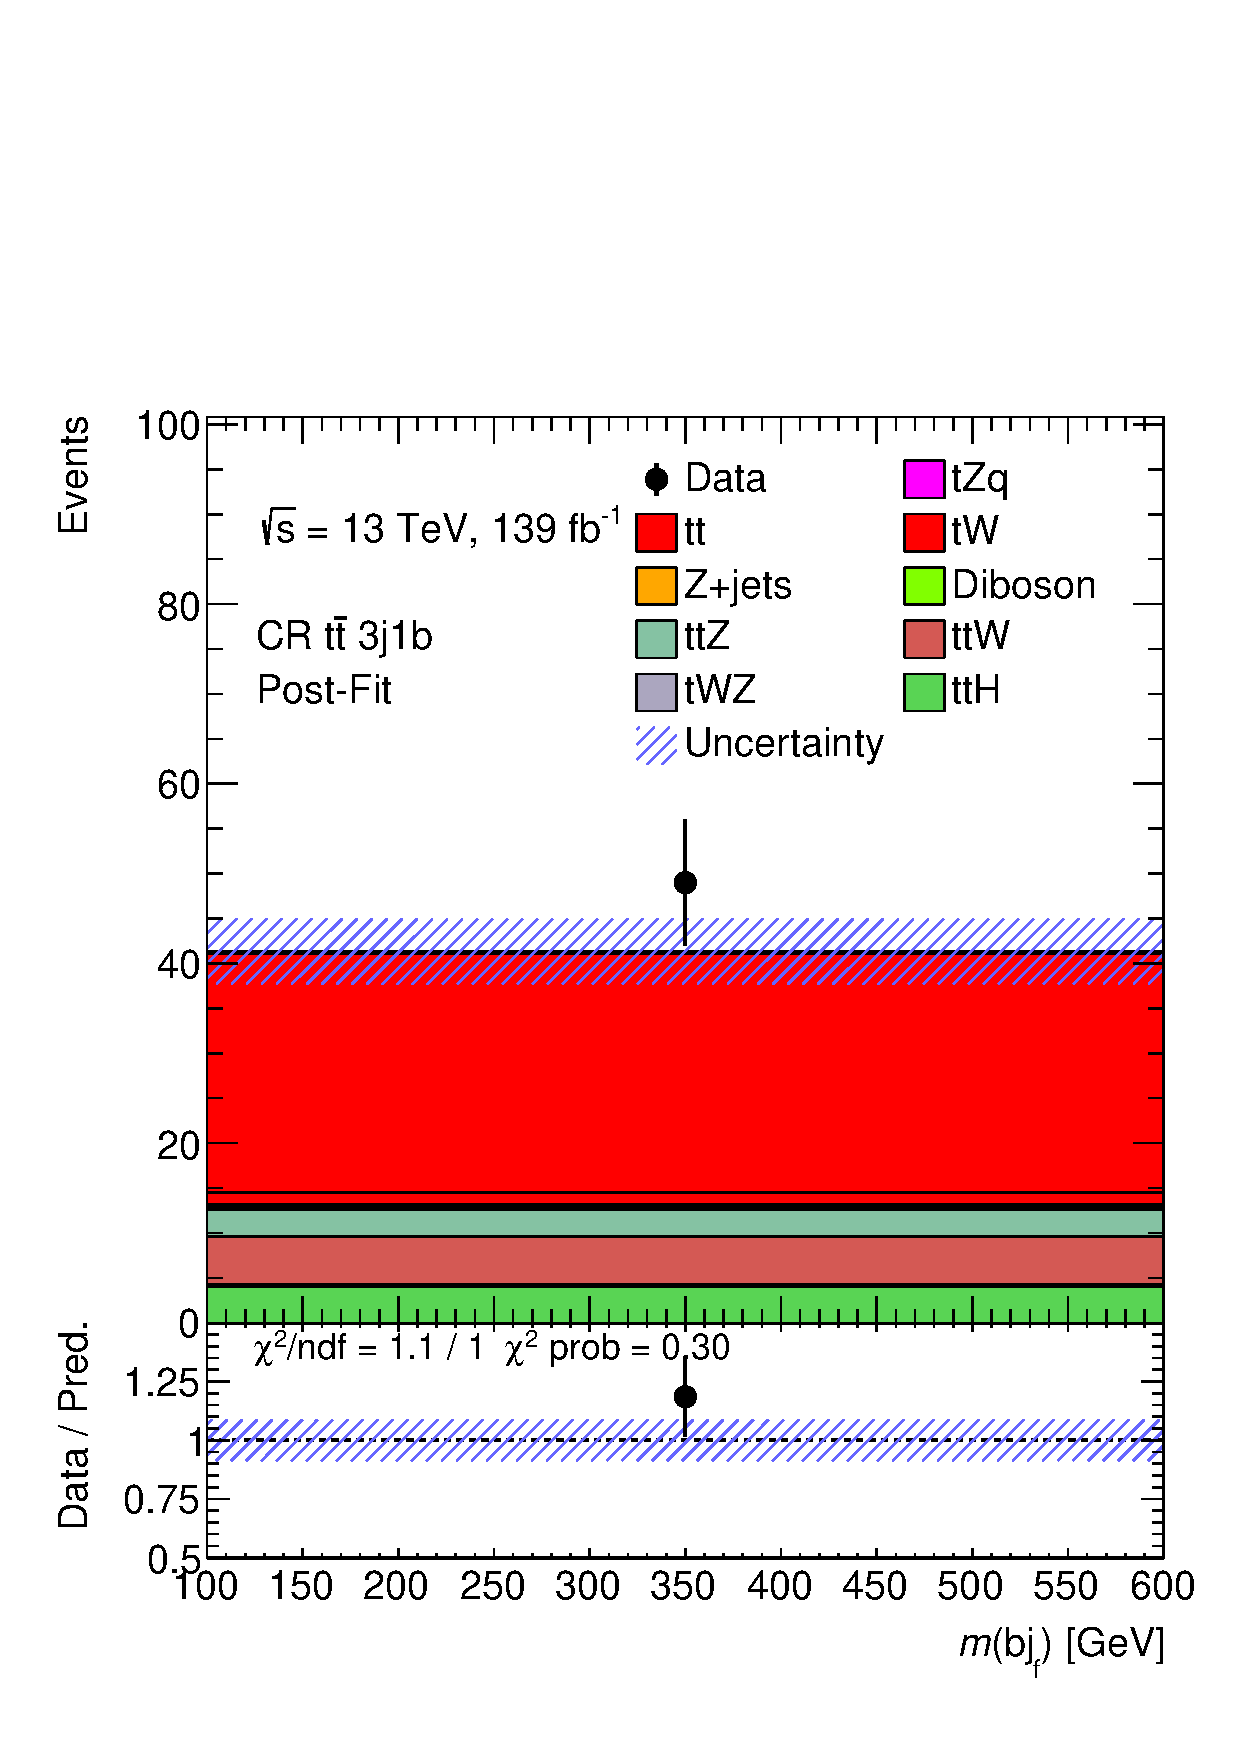
\includegraphics[width=\textwidth]{ubonn-thesis/Chapters/Chapters_07/Figure/Data/CR_3j1b_postFit.pdf} 
   \caption{}
  \end{subfigure}%% 
  \caption{Pre-fit and post-fit distributions in the signal regions and control regions described in the table \ref{tab:fittedregions}. The black points show the unblinded dataset. The error band includes the statistical and systematic uncertainties. $\chi^{2}-$value, number of degree of freedom, and corresponding p-vale of $\chi^{2}$ fit are shown in ratio plot.}
  \label{fig:datafit2}
  \end{figure}

%% Yield table

\begin{table}[h!]
    \centering
    \begin{adjustbox}{width=\textwidth}
    \begin{tabular}{@{} *9l  @{}}
    \toprule
     & SR 2j1b & SR 3j1b & CR $t\Bar{t}Z$ 3j2b & CR $t\Bar{t}Z$ 4j2b & CR diboson 2j0b & CR diboson 3j0b & CR $t\Bar{t}$ 2j1b & CR $t\Bar{t}$ 3j1b \\
\midrule
  tZq   & 97.5 $\pm$ 11.3 & 55.3 $\pm$ 6.4 & 15.8 $\pm$ 1.9 & 10.4 $\pm$ 1.2 & 61.9 $\pm$ 7.2 & 25.6 $\pm$ 3.0 & 0.3 $\pm$ 0.1 & 0.2 $\pm$ 0.1 \\ 
  tt   & 30.2 $\pm$ 1.7 & 14.3 $\pm$ 1.0 & 3.1 $\pm$ 0.4 & 1.5 $\pm$ 0.3 & 19.4 $\pm$ 1.2 & 7.4 $\pm$ 0.7 & 57.7 $\pm$ 3.1 & 27.0 $\pm$ 1.6 \\ 
  tW   & 1.2 $\pm$ 0.5 & 0.4 $\pm$ 0.4 & 0.1 $\pm$ 0.1 & 0.2 $\pm$ 0.2 & 0.7 $\pm$ 0.4 & 0.8 $\pm$ 0.4 & 3.1 $\pm$ 0.7 & 1.4 $\pm$ 0.5 \\ 
  Z+jets   & 79.9 $\pm$ 9.8 & 29.0 $\pm$ 2.8 & 2.4 $\pm$ 0.4 & 1.2 $\pm$ 0.3 & 332.1 $\pm$ 43.6 & 114.5 $\pm$ 13.7 & 0.4 $\pm$ 0.3 & 0.3 $\pm$ 0.3 \\ 
  Diboson   & 115.6 $\pm$ 34.9 & 66.1 $\pm$ 19.9 & 5.5 $\pm$ 1.7 & 3.4 $\pm$ 1.0 & 2625.6 $\pm$ 791.4 & 973.5 $\pm$ 293.4 & 0.4 $\pm$ 0.1 & 0.3 $\pm$ 0.1 \\ 
  ttZ   & 79.9 $\pm$ 3.7 & 128.8 $\pm$ 3.8 & 62.2 $\pm$ 2.1 & 67.8 $\pm$ 2.3 & 61.7 $\pm$ 6.4 & 59.9 $\pm$ 2.7 & 3.4 $\pm$ 0.2 & 3.1 $\pm$ 0.2 \\ 
  ttW   & 4.6 $\pm$ 0.7 & 2.3 $\pm$ 0.4 & 1.7 $\pm$ 0.3 & 0.8 $\pm$ 0.1 & 1.9 $\pm$ 0.3 & 0.9 $\pm$ 0.2 & 9.8 $\pm$ 1.5 & 5.2 $\pm$ 0.8 \\ 
  tWZ   & 19.3 $\pm$ 0.8 & 22.9 $\pm$ 0.9 & 3.9 $\pm$ 0.3 & 4.8 $\pm$ 0.3 & 17.1 $\pm$ 0.7 & 13.1 $\pm$ 0.7 & 0.4 $\pm$ 0.1 & 0.3 $\pm$ 0.1 \\ 
  ttH   & 2.1 $\pm$ 0.3 & 2.8 $\pm$ 0.4 & 1.6 $\pm$ 0.2 & 1.4 $\pm$ 0.2 & 1.1 $\pm$ 0.2 & 1.1 $\pm$ 0.2 & 3.3 $\pm$ 0.5 & 3.9 $\pm$ 0.6 \\ 
\midrule
  Total  & 430.2 $\pm$ 40.2 & 322.0 $\pm$ 23.2 & 96.2 $\pm$ 4.1 & 91.4 $\pm$ 3.5 & 3121.4 $\pm$ 794.4 & 1196.7 $\pm$ 294.5 & 78.9 $\pm$ 4.4 & 41.7 $\pm$ 2.5 \\ 
\midrule 
  Data   & 443 & 307 & 118 & 77 & 3116 & 1083 & 71 & 49 \\ 
      \bottomrule
 \end{tabular}
 \end{adjustbox}
 \caption{Pre-fit: Observed yields in each of the analysis regions considered. The signal and background predictions are shown before the fit to data. The quoted uncertainties include the statistical and systematic uncertainties of the yields.}
 \label{tab:prefityield}
 \end{table}

\begin{table}[h!]
    \centering
    \begin{adjustbox}{width=\textwidth}
    \begin{tabular}{@{} *9l  @{}}
    \toprule
     & SR 2j1b & SR 3j1b & CR $t\Bar{t}Z$ 3j2b & CR $t\Bar{t}Z$ 4j2b & CR diboson 2j0b & CR diboson 3j0b & CR $t\Bar{t}$ 2j1b & CR $t\Bar{t}$ 3j1b \\
\midrule
  tZq   & 126.9 $\pm$  11.7 & 71.8 $\pm$  6.7 & 20.6 $\pm$  1.9 & 13.6 $\pm$  1.3 & 80.8 $\pm$  7.6 & 33.0 $\pm$  3.2 & 0.4 $\pm$  0.1 & 0.7 $\pm$  0.1 \\ 
  tt   & 29.4 $\pm$  3.9 & 14.0 $\pm$  1.9 & 3.0 $\pm$  0.4 & 1.5 $\pm$  0.2 & 19.1 $\pm$  2.6 & 7.2 $\pm$  2.0 & 56.4 $\pm$  7.4 & 26.5 $\pm$  3.5 \\ 
  tW   & 1.1 $\pm$  0.2 & 0.4 $\pm$  0.1 & 0.1 $\pm$  0.0 & 0.2 $\pm$  0.0 & 0.6 $\pm$  0.1 & 0.8 $\pm$  0.1 & 3.0 $\pm$  0.4 & 1.4 $\pm$  0.2 \\ 
  Z+jets   & 77.0 $\pm$  9.5 & 28.9 $\pm$  3.7 & 2.4 $\pm$  0.3 & 1.2 $\pm$  0.2 & 336.9 $\pm$  42.4 & 112.9 $\pm$  14.4 & 0.4 $\pm$  0.1 & 0.3 $\pm$  0.1 \\ 
  Diboson   & 109.3 $\pm$  3.4 & 63.0 $\pm$  1.6 & 5.3 $\pm$  0.2 & 3.2 $\pm$  0.1 & 2523.7 $\pm$  62.3 & 926.7 $\pm$  22.8 & 0.4 $\pm$  0.0 & 0.3 $\pm$  0.0 \\ 
  ttZ   & 73.6 $\pm$  6.7 & 119.6 $\pm$  10.7 & 58.2 $\pm$  5.2 & 63.2 $\pm$  5.6 & 57.8 $\pm$  5.5 & 55.3 $\pm$  5.2 & 3.2 $\pm$  0.3 & 2.9 $\pm$  0.3 \\ 
  ttW   & 4.6 $\pm$ 0.7 & 2.4 $\pm$  0.4 & 1.7 $\pm$  0.3 & 0.8 $\pm$  0.1 & 1.9 $\pm$  0.3 & 0.9 $\pm$  0.1 & 9.9 $\pm$  1.5 & 5.3 $\pm$  0.8 \\ 
  tWZ   & 19.2 $\pm$  0.6 & 22.9 $\pm$  0.7 & 3.9 v 0.1 & 4.8 $\pm$ 0.2 & 17.2 $\pm$  0.5 & 13.0 $\pm$  0.4 & 0.4 $\pm$  0.0 & 0.3 $\pm$  0.0 \\ 
  ttH   & 2.1 $\pm$  0.3 & 2.9 $\pm$  0.4 & 1.6 $\pm$  0.2 & 1.4 $\pm$  0.2 & 1.2 $\pm$  0.2 & 1.1 $\pm$  0.2 & 3.4 $\pm$  0.5 & 4.0 $\pm$  0.6 \\ 
\hline 
  Total  & 443.2 $\pm$  14.0 & 325.9 $\pm$  10.6 & 96.8 $\pm$  5.0 & 89.9 $\pm$  5.4 & 3039.1 $\pm$  47.8 & 1150.9 $\pm$  19.0 & 77.6 $\pm$  7.4 & 41.3 $\pm$  3.6 \\ 
\hline 
  Data   & 443 & 307 & 118 & 77 & 3116 & 1083 & 71 & 49 \\ 
\bottomrule
 \end{tabular}
 \end{adjustbox}
 \caption{Post-fit: Observed yields in each of the analysis regions considered. The signal and background predictions are shown after the fit to data. The quoted uncertainties include the statistical and systematic uncertainties of the yields.}
 \label{tab:postfityield}
 \end{table}


\begin{table}[!h]
    \begin{minipage}{.49\textwidth}
      \centering
      \begin{adjustbox}{width=0.8\textwidth}
       \begin{tabular}{@{} *4l  @{}}
      \toprule
      Uncertainty source & $\Delta \sigma /\sigma$[\%]\\
     \midrule
      Signal &  14.3  \\[0.2ex]
      Background &  1.9  \\[0.2ex]
      Electron &   2.7 \\[0.2ex]
      Muon  &  2.2  \\[0.2ex]
      Jet &   1.1  \\[0.2ex]
     Luminosity  &  2.2  \\[0.2ex]
     Pile-up  &  1.5  \\[0.2ex]
     b-tagging  &  0.8  \\[0.2ex]
     \midrule
     Total systematic uncertainty &   17.2 \\[0.2ex]
     \bottomrule
 \end{tabular}
 \end{adjustbox}
    \end{minipage}%
    \hfill
    %\hspace{-1.5cm}
    \begin{minipage}{.49\textwidth}
      \centering
      \vspace*{0.5cm}
      \begin{adjustbox}{width=\textwidth}
        \begin{tabular}{@{} *4l  @{}}
      \toprule
      Uncertainty source & $\Delta \sigma /\sigma$[\%]\\
     \midrule
     Data statistics & 9.2 \\[0.2ex]
     $t\Bar{t}$ + tW, Z + jets, and $t\Bar{t}Z$ normalisation & 2.2 \\[0.2ex]
     Gammas  &  1.2  \\[0.2ex]
     \midrule
     Total statistical uncertainty & 12.0 \\[0.2ex]
     \bottomrule
 \end{tabular}
 \end{adjustbox}
\end{minipage} 
\caption{ Impact of systematic uncertainties on the tZq cross-section, broken down into major categories. MC statistics refers to the effect of the limited size of the MC samples. The total systematic uncertainty is a bit larger than the quadratic sum of the individual contributions due to correlations.}
\label{tab:impact_table}
\end{table}



\begin{figure}[!h] 
  \begin{subfigure}[b]{0.49\linewidth}
    \centering
    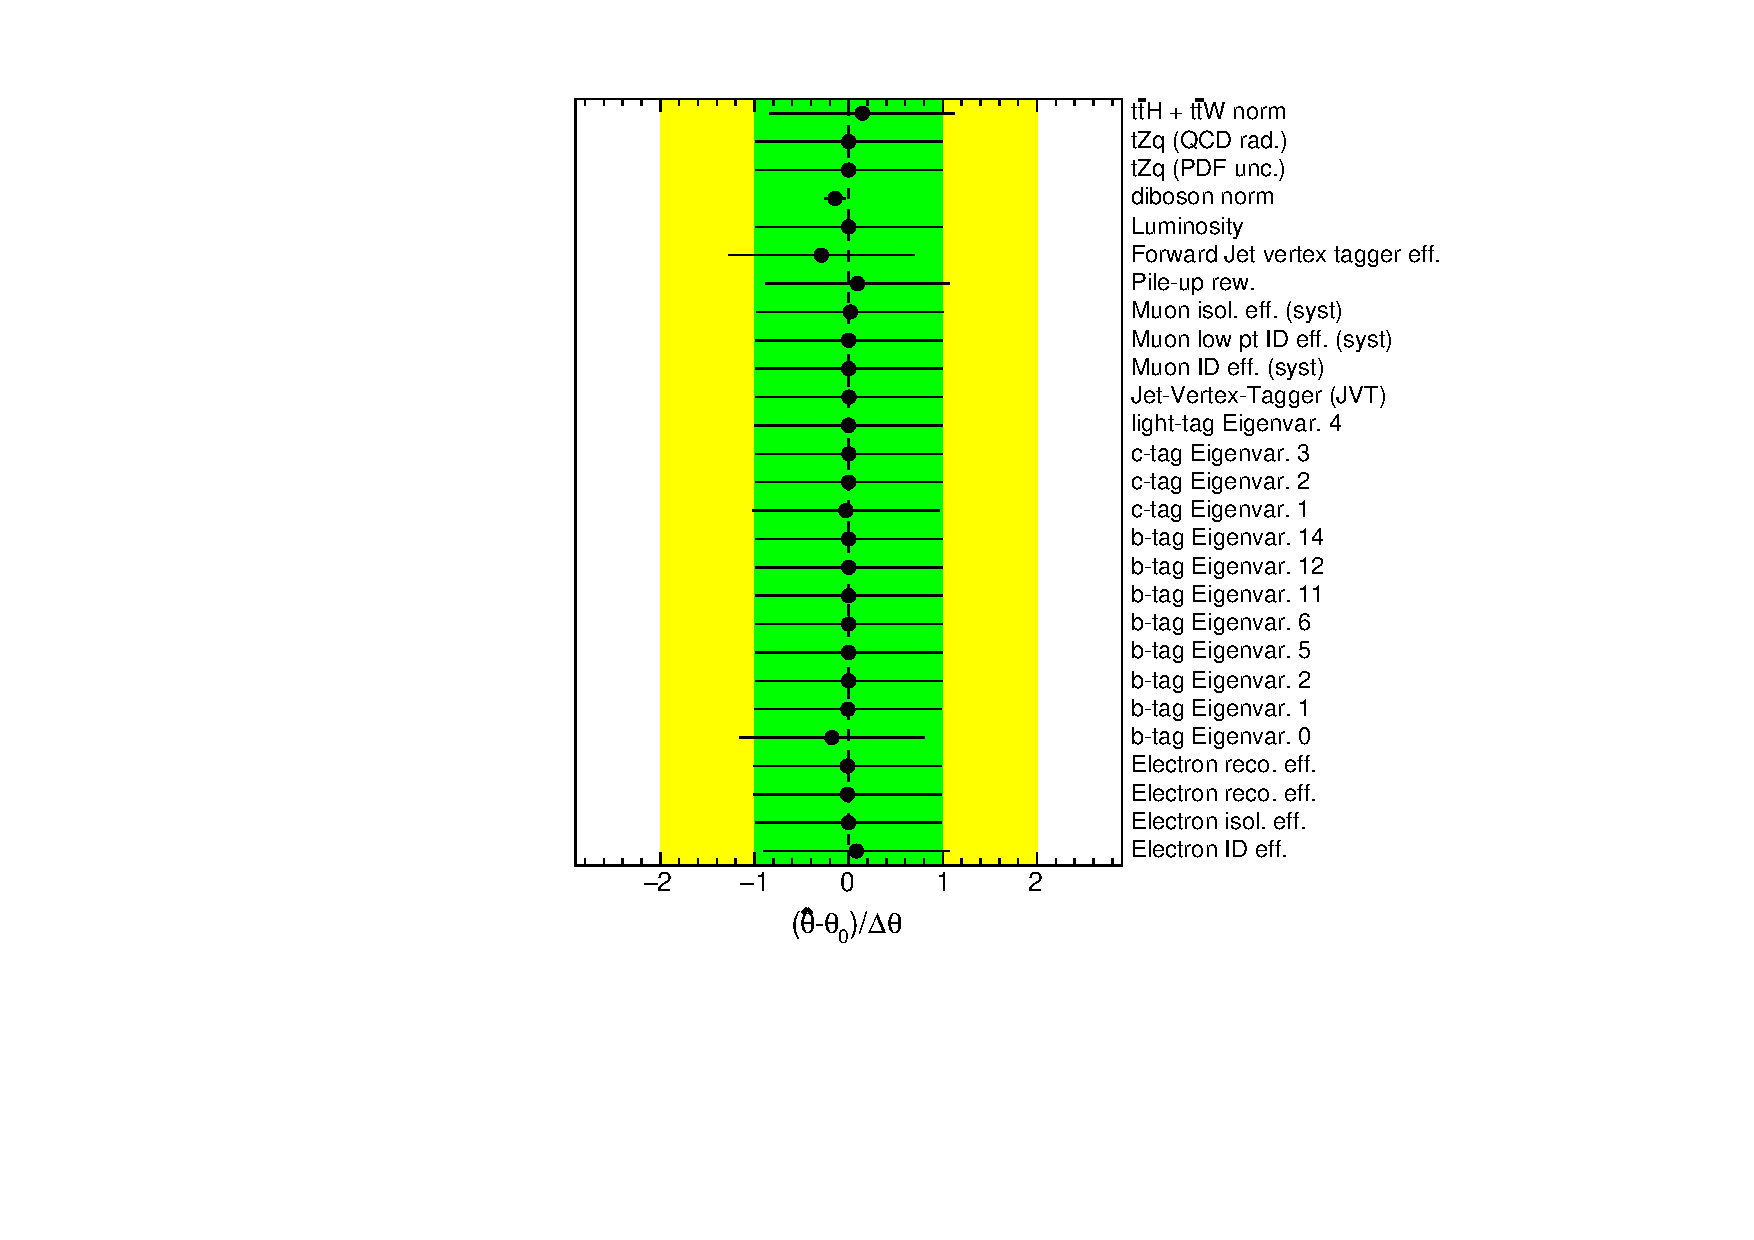
\includegraphics[width=1.3\textwidth]{ubonn-thesis/Chapters/Chapters_07/Figure/Data/NuisPar.pdf}
    \caption{}
    \label{fig:datapull}
  \end{subfigure}%% 
  \begin{subfigure}[b]{0.49\linewidth}
    \centering
    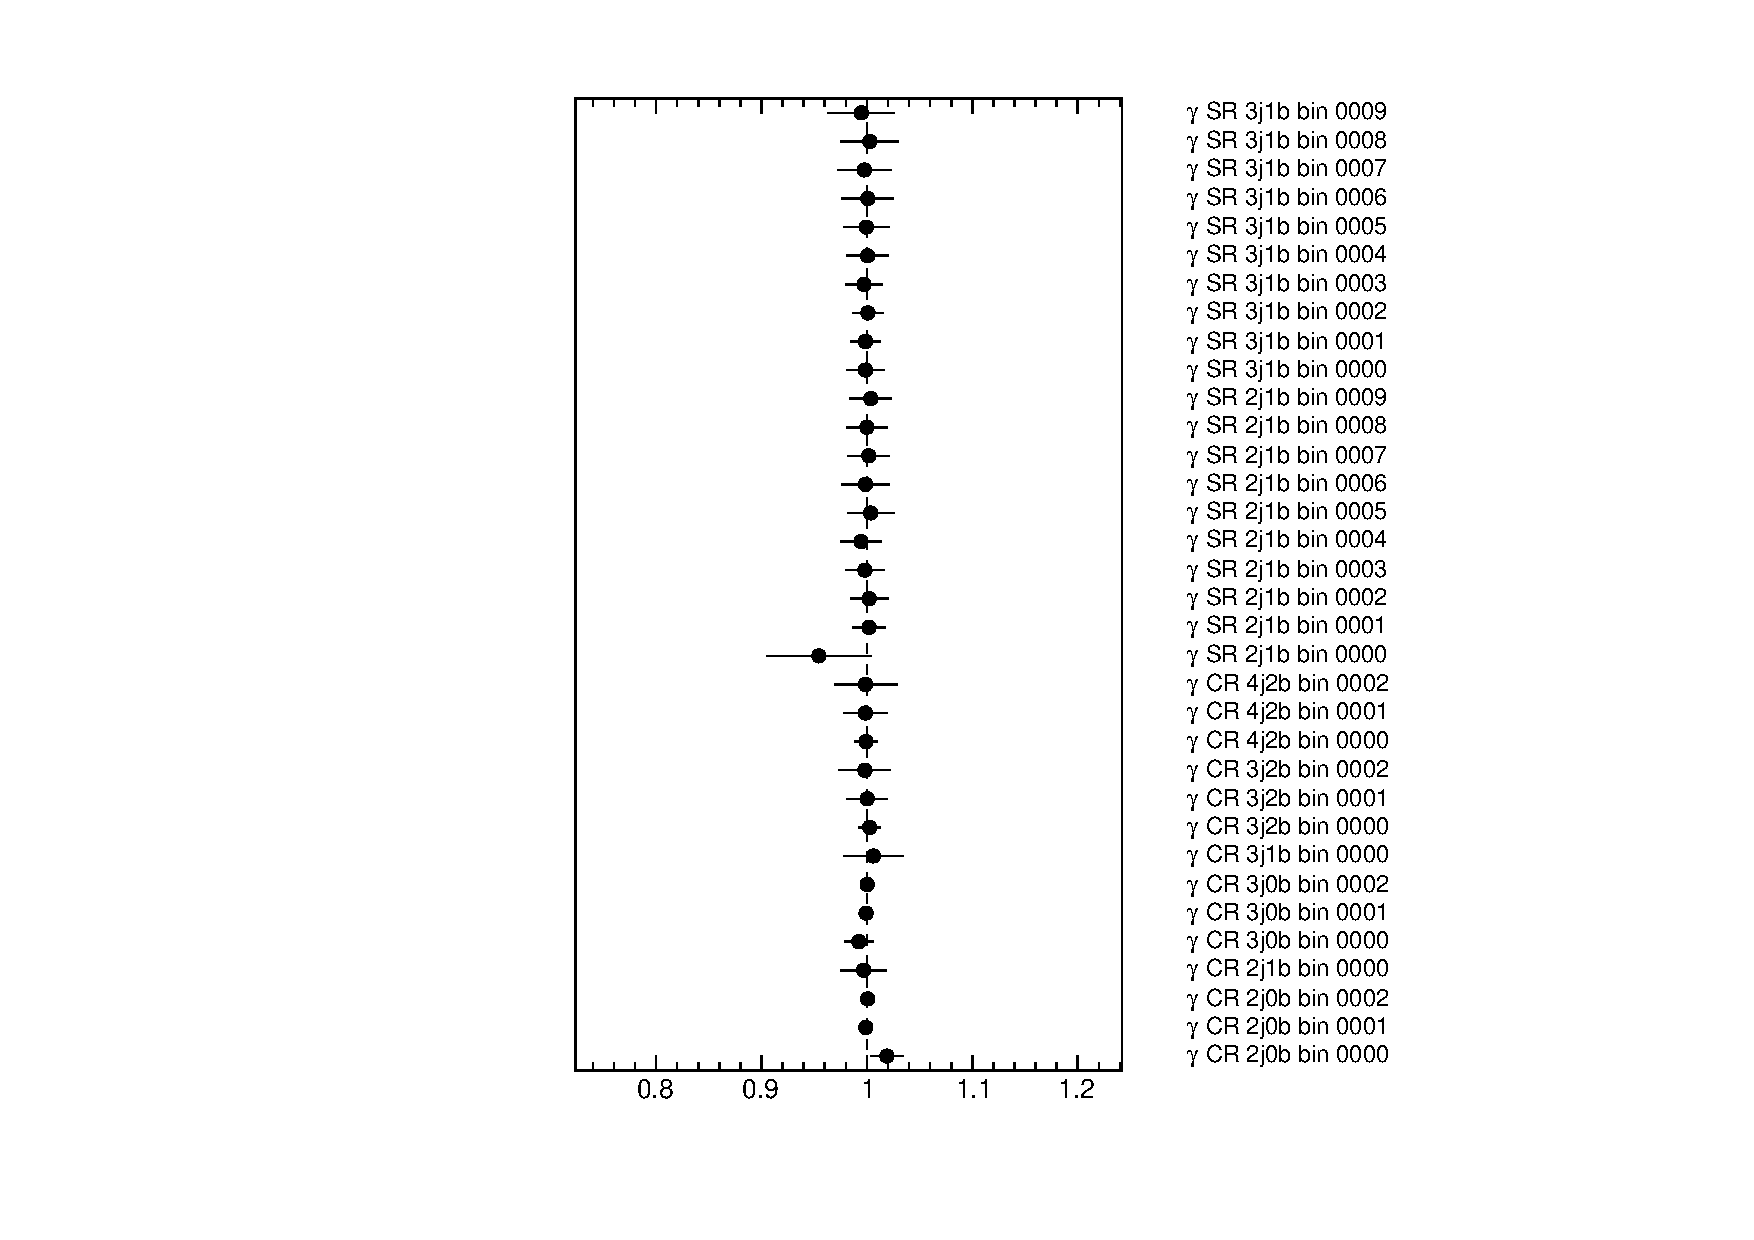
\includegraphics[width=1.1\textwidth]{ubonn-thesis/Chapters/Chapters_07/Figure/Data/Gammas.pdf}
   \caption{}
  \end{subfigure}
  \caption{(a) Pull distributions of nuisance parameters associated to systematic uncertainties using the full unblinded dataset. Only nuisance parameters substantial effect are shown. (b) Pull distributions of bin gamma parameters in the unblinded fit.}
\end{figure}

\begin{figure}[!h]
    \centering
    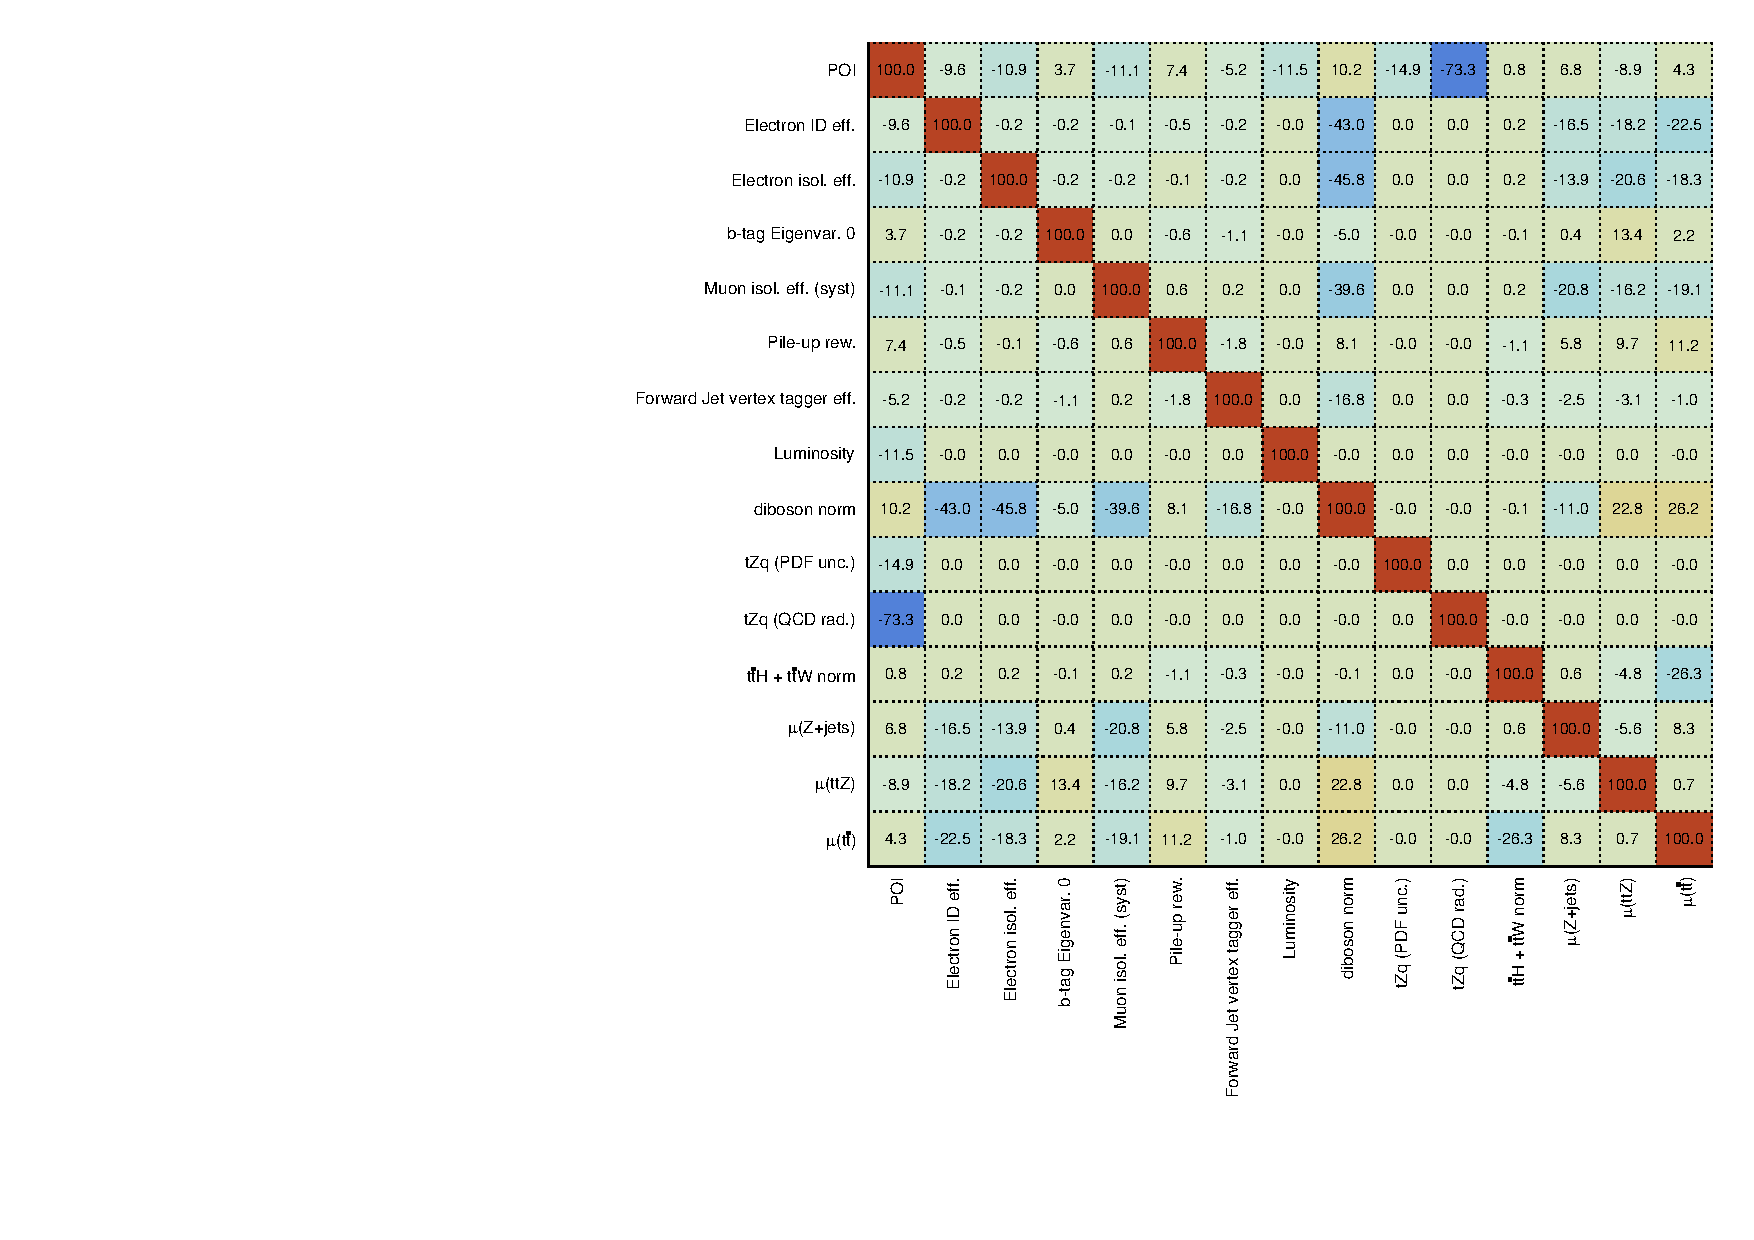
\includegraphics[width=0.6\textwidth]{ubonn-thesis/Chapters/Chapters_07/Figure/Data/CorrMatrix.pdf}
    \caption{ Correlation matrix of the parameters included in the likelihood fit for the data.}
    \label{fig:correlation}
\end{figure}

\begin{figure}[!h] 
  \begin{subfigure}[b]{0.48\linewidth}
    \centering
    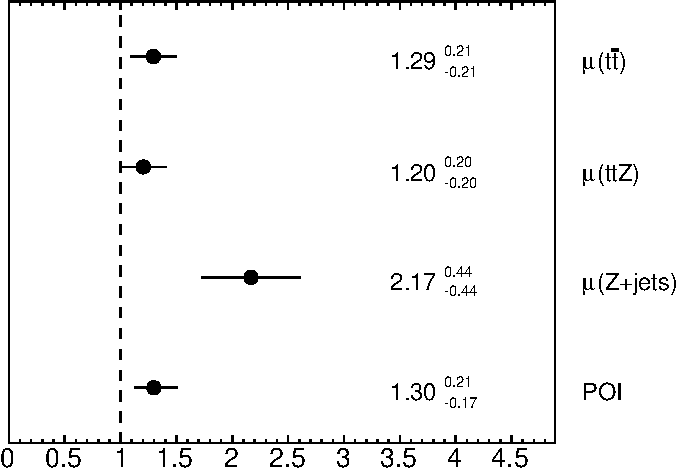
\includegraphics[width=\textwidth]{ubonn-thesis/Chapters/Chapters_07/Figure/Data/NormFactors-crop.pdf}
    \caption{}
    \label{fig:statsyst}
  \end{subfigure}%% 
  \begin{subfigure}[b]{0.48\linewidth}
    \centering
    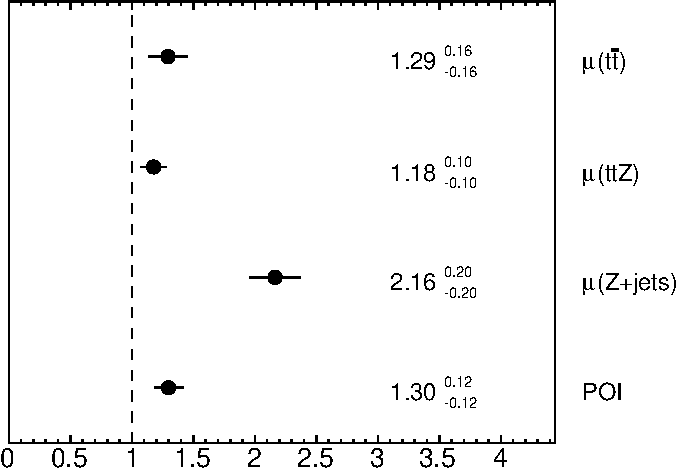
\includegraphics[width=\textwidth]{ubonn-thesis/Chapters/Chapters_07/Figure/Data/NormFactors_statOnly-crop.pdf}
   \caption{}
   \label{fig:statonly}
  \end{subfigure}
  \caption{Norm factors of the free floating parameters during the binned profile likelihood fit in the signal regions and control regions for the data.(a) Syst + Stat fit (b) Statonly fit}
\end{figure}

\begin{figure}[!h] 
  \begin{subfigure}[b]{0.49\linewidth}
    \centering
    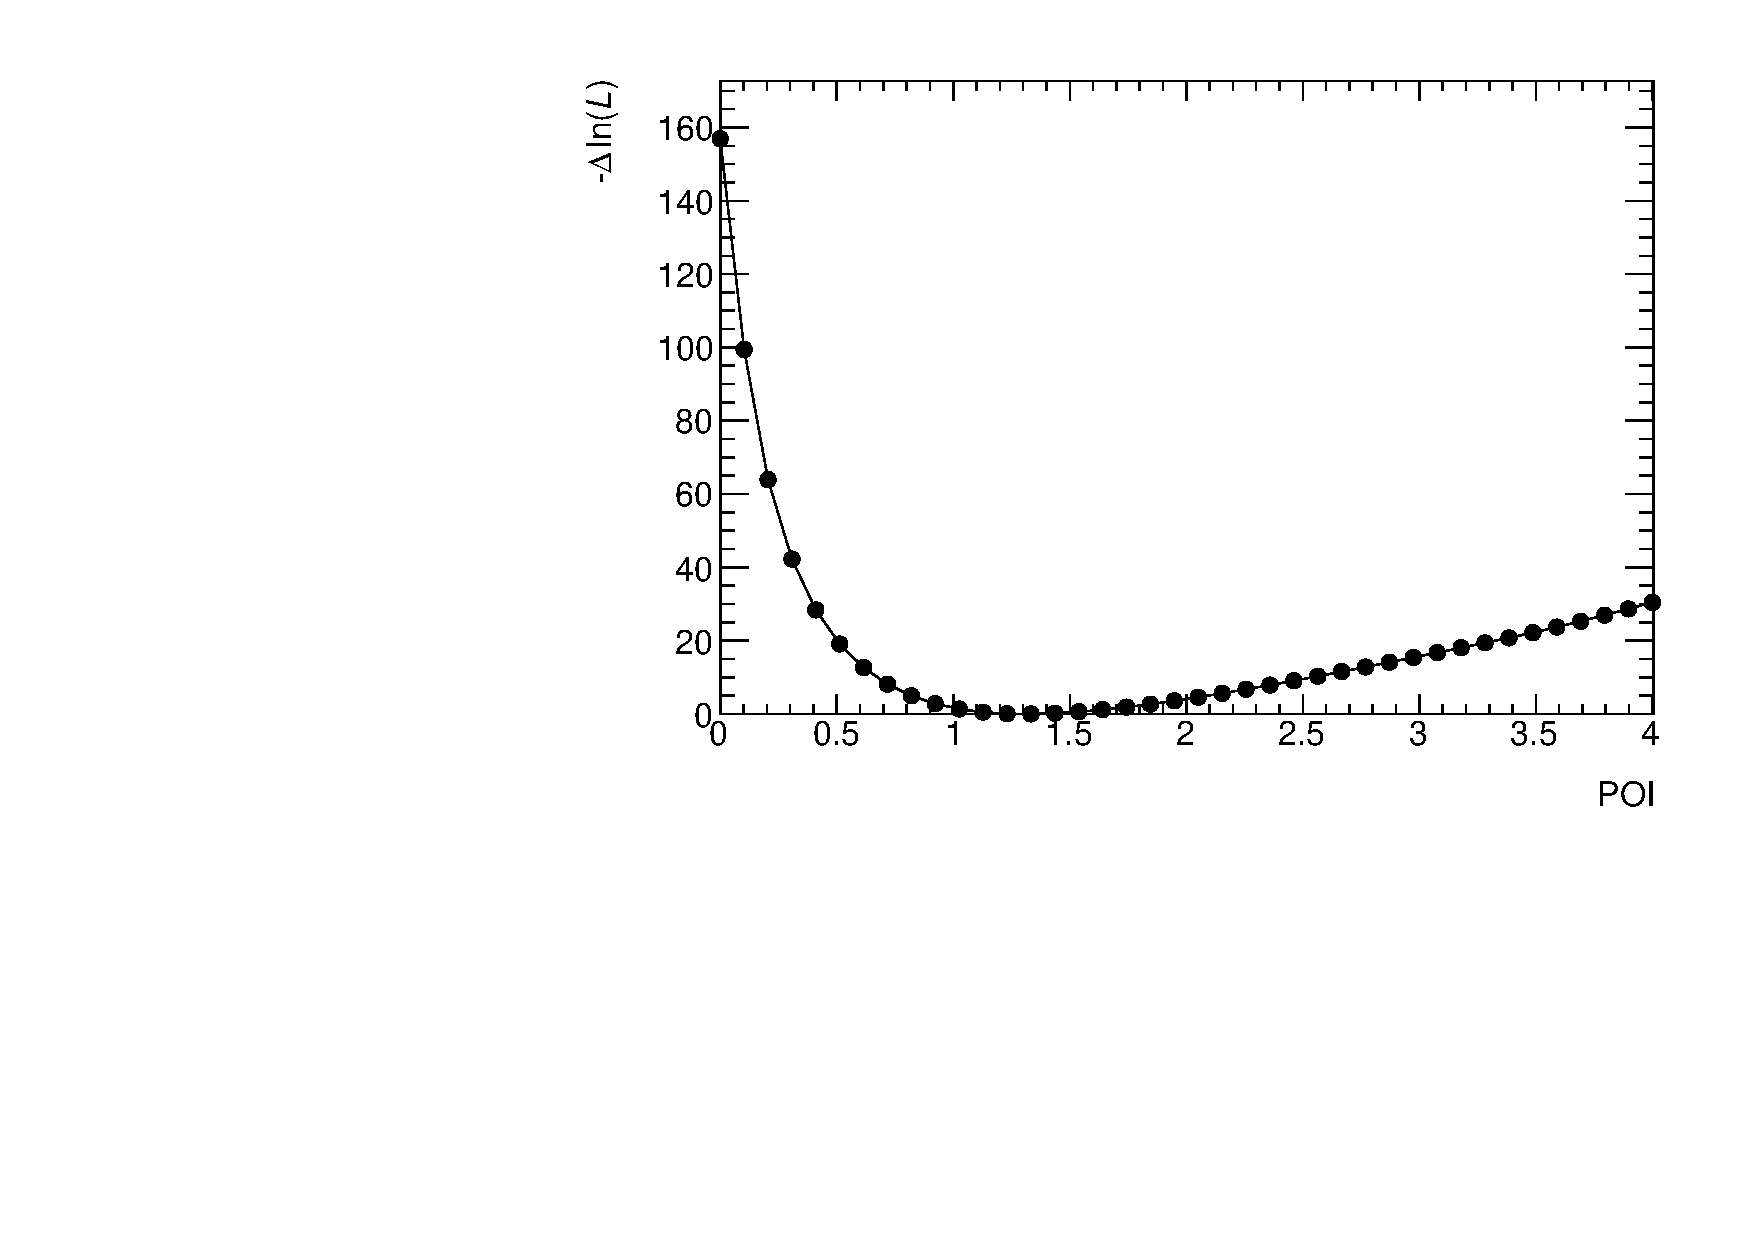
\includegraphics[width=\textwidth]{ubonn-thesis/Chapters/Chapters_07/Figure/Data/NLLscan_POI.pdf}
    \caption{}
    \label{fig:dataNLL}
  \end{subfigure}%% 
  \begin{subfigure}[b]{0.49\linewidth}
    \centering
    \hspace*{0.4cm}
    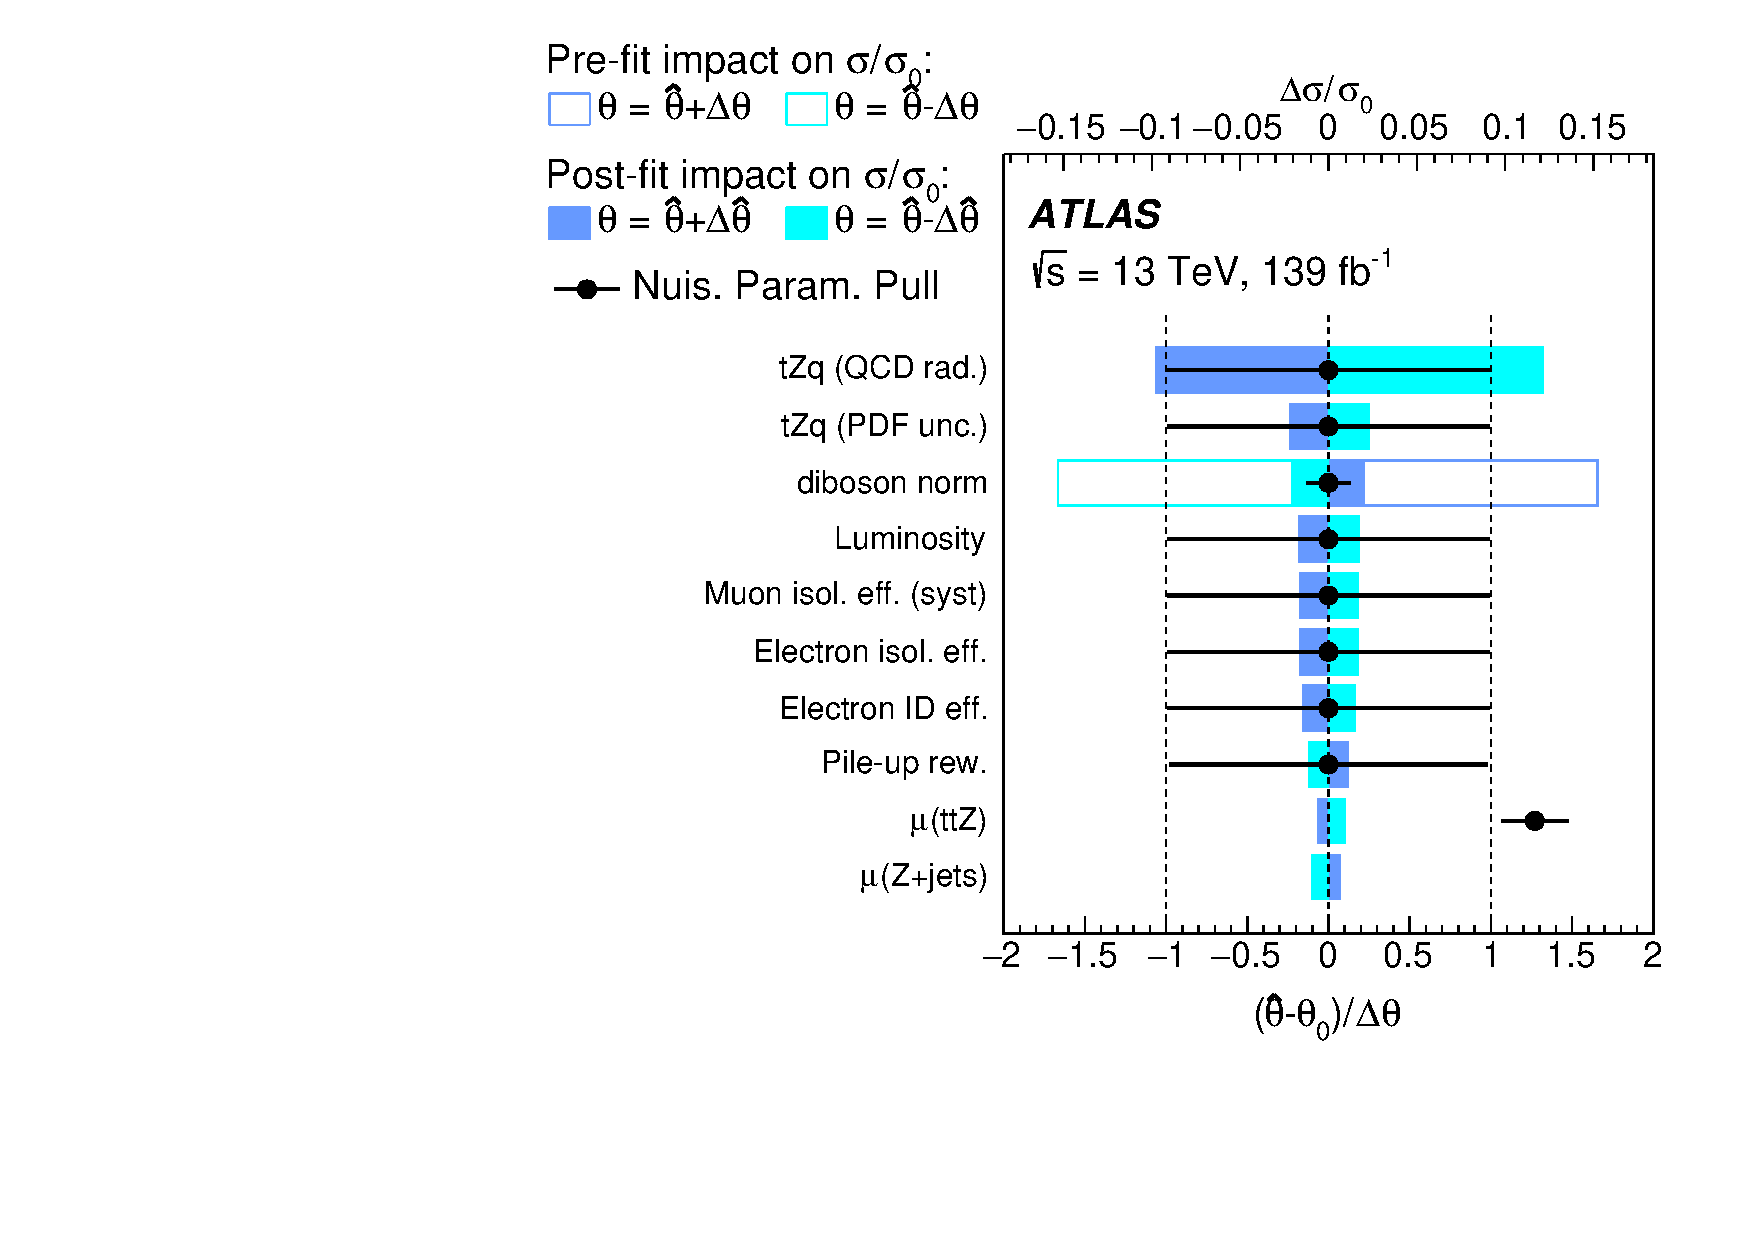
\includegraphics[width=\textwidth]{ubonn-thesis/Chapters/Chapters_07/Figure/Data/RankingSysts_POI_systs.pdf}
   \caption{}
   \label{fig:datarank}
  \end{subfigure}
  \caption{(a) The likelihood scan of the signal strength ($\mu$) or parameter of interest (POI) and (b) The ranking plot showing the impact of each NP on $\mu$ in the unblinded fit. There, the empty/full boxes show the pre-/post-fit impacts while the black dots/lines represent the post-fit values/uncertainties of all NPs. Only the 10 NPs with the highest post-fit impacts are displayed. }
\end{figure}

%%%  tZq rad systematics

\begin{figure}[!h] 
  \begin{subfigure}[b]{0.33\linewidth}
    \centering
    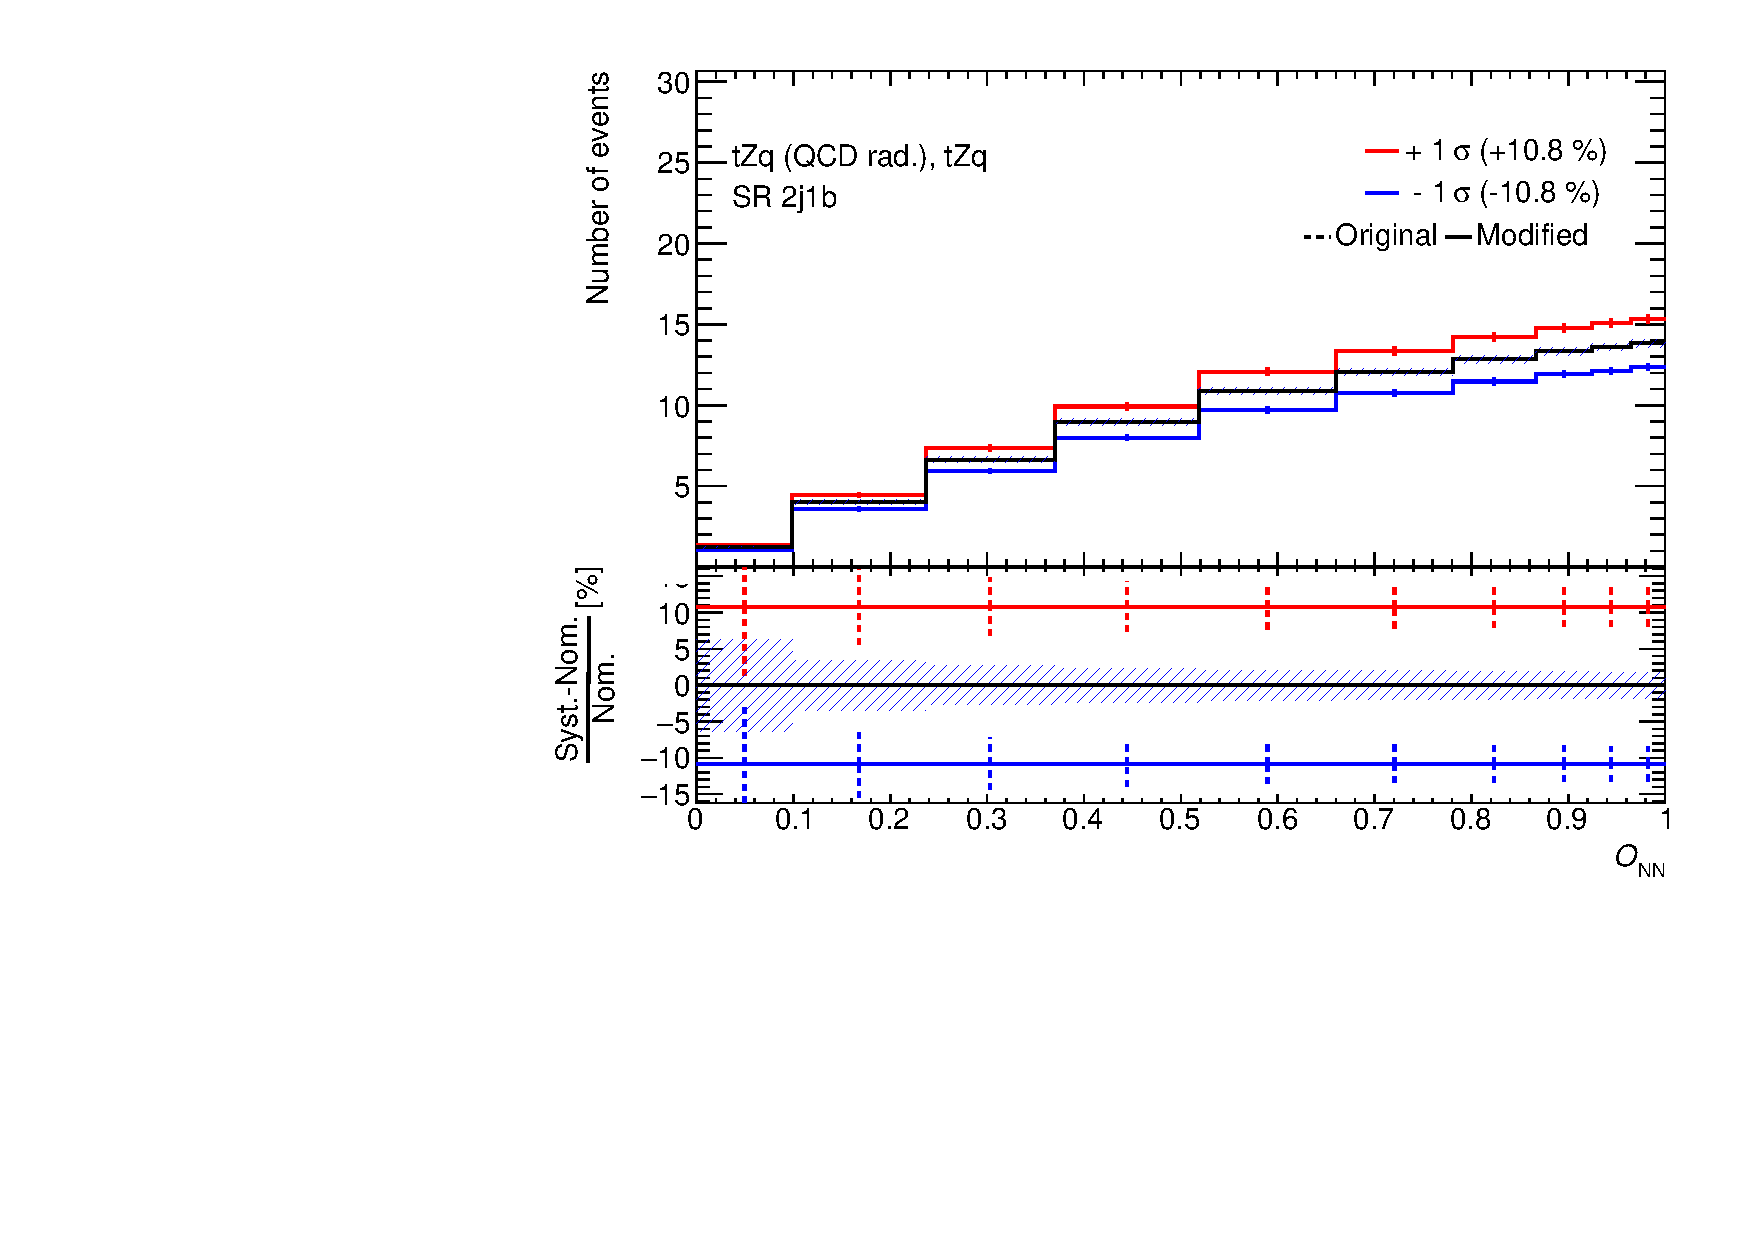
\includegraphics[width=\textwidth]{ubonn-thesis/Chapters/Chapters_07/Figure/Data/Systematic/tZq_qcdrad/SR_2j1b_tZq_tZq_XS_QCDscale.pdf} 
    \caption{}
  \end{subfigure}%% 
  \begin{subfigure}[b]{0.33\linewidth}
    \centering
    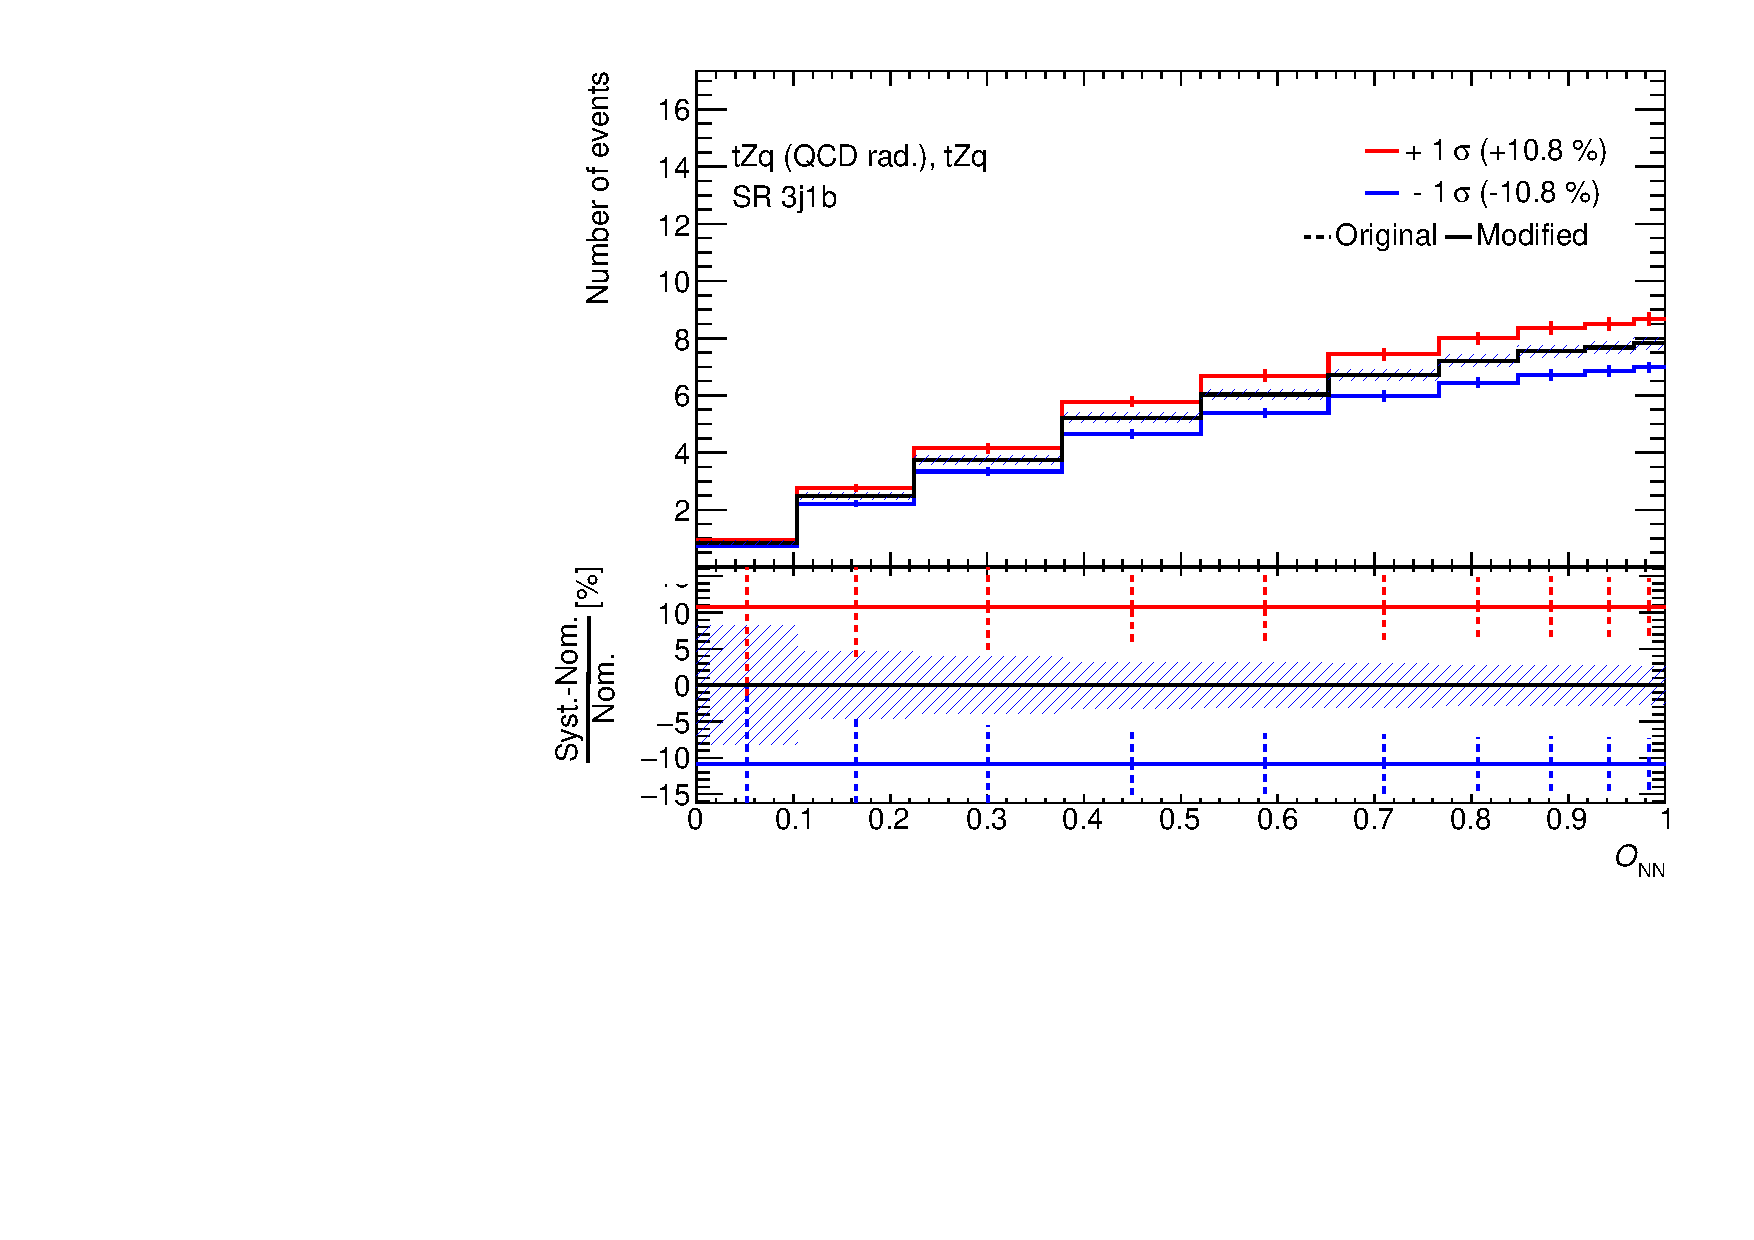
\includegraphics[width=\textwidth]{ubonn-thesis/Chapters/Chapters_07/Figure/Data/Systematic/tZq_qcdrad/SR_3j1b_tZq_tZq_XS_QCDscale.pdf} 
    \caption{}
  \end{subfigure} 
  \begin{subfigure}[b]{0.33\linewidth}
    \centering
    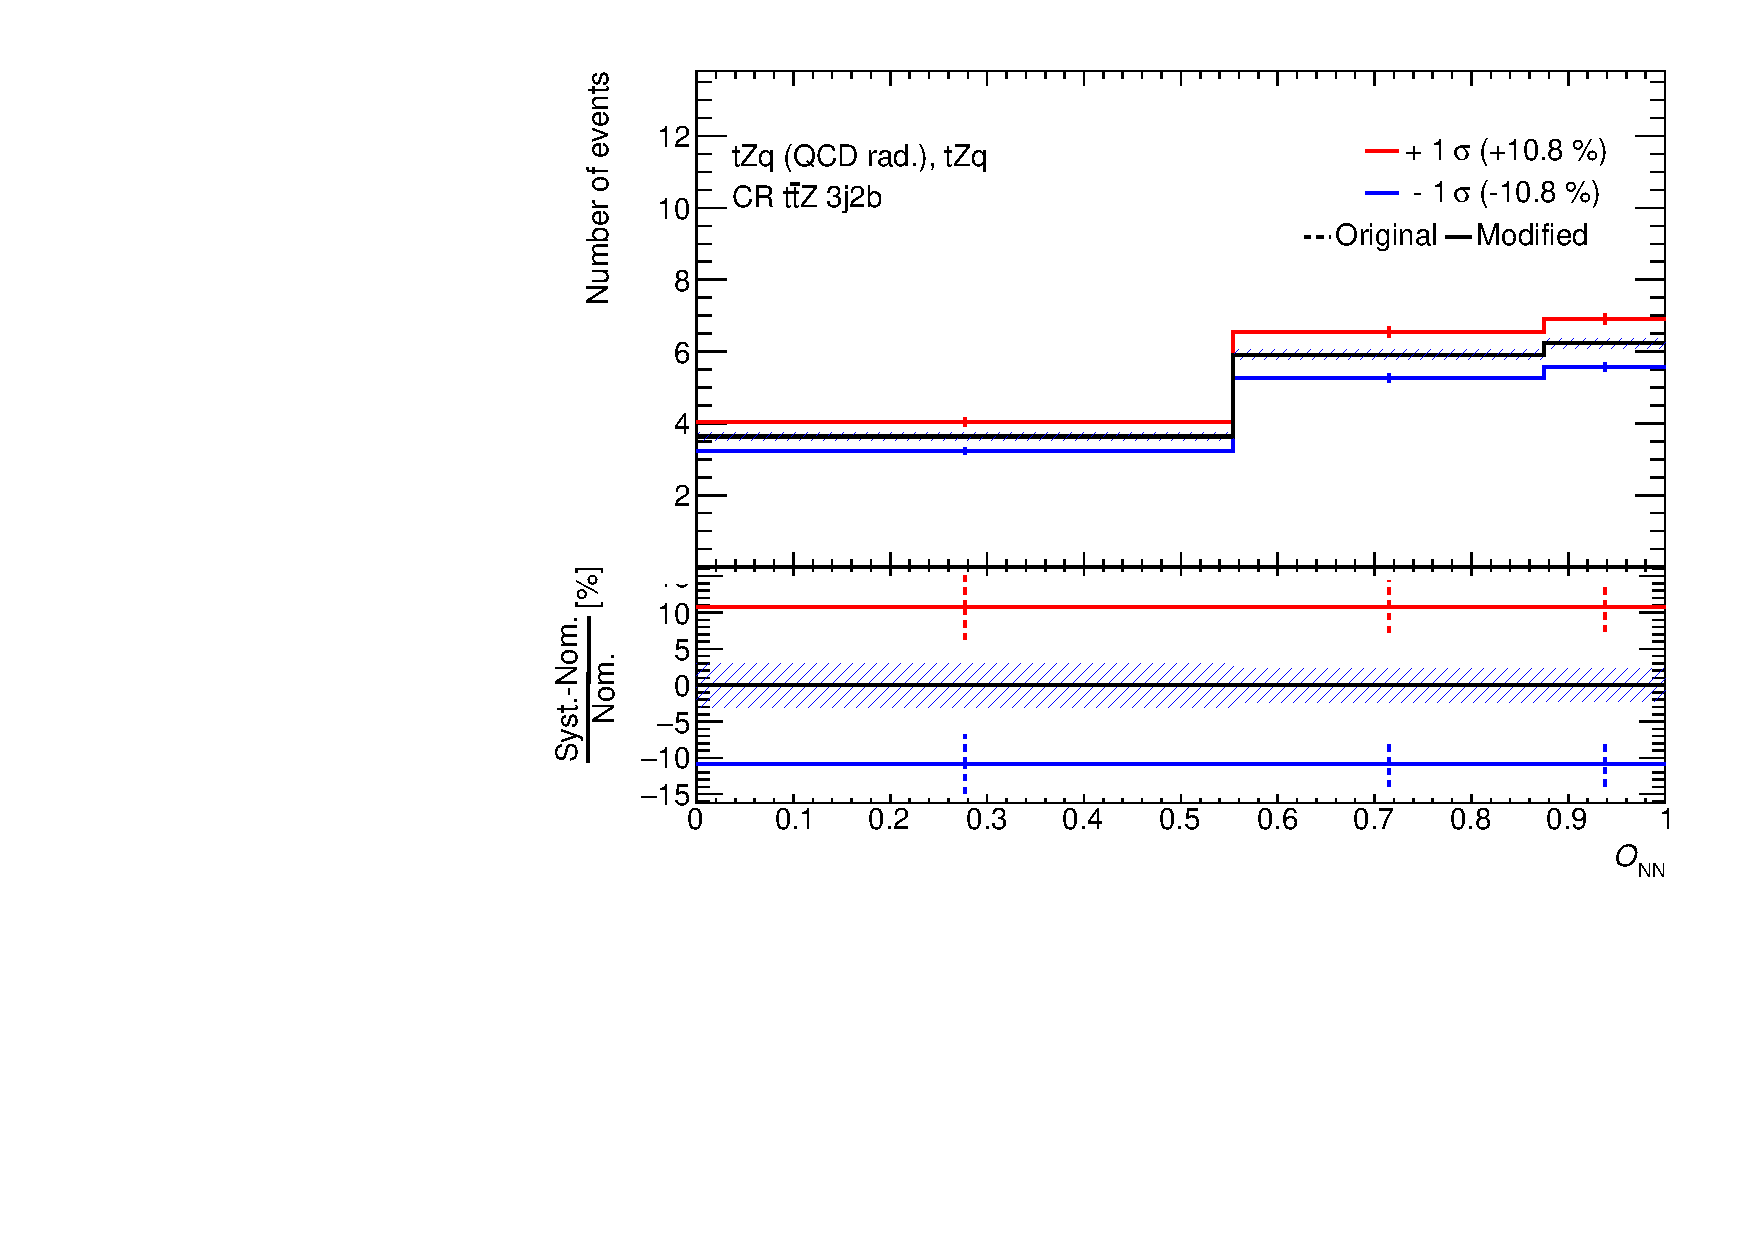
\includegraphics[width=\textwidth]{ubonn-thesis/Chapters/Chapters_07/Figure/Data/Systematic/tZq_qcdrad/CR_3j2b_tZq_tZq_XS_QCDscale.pdf} 
    \caption{}
  \end{subfigure}%%
  \newline
  \begin{subfigure}[b]{0.33\linewidth}
  \centering
    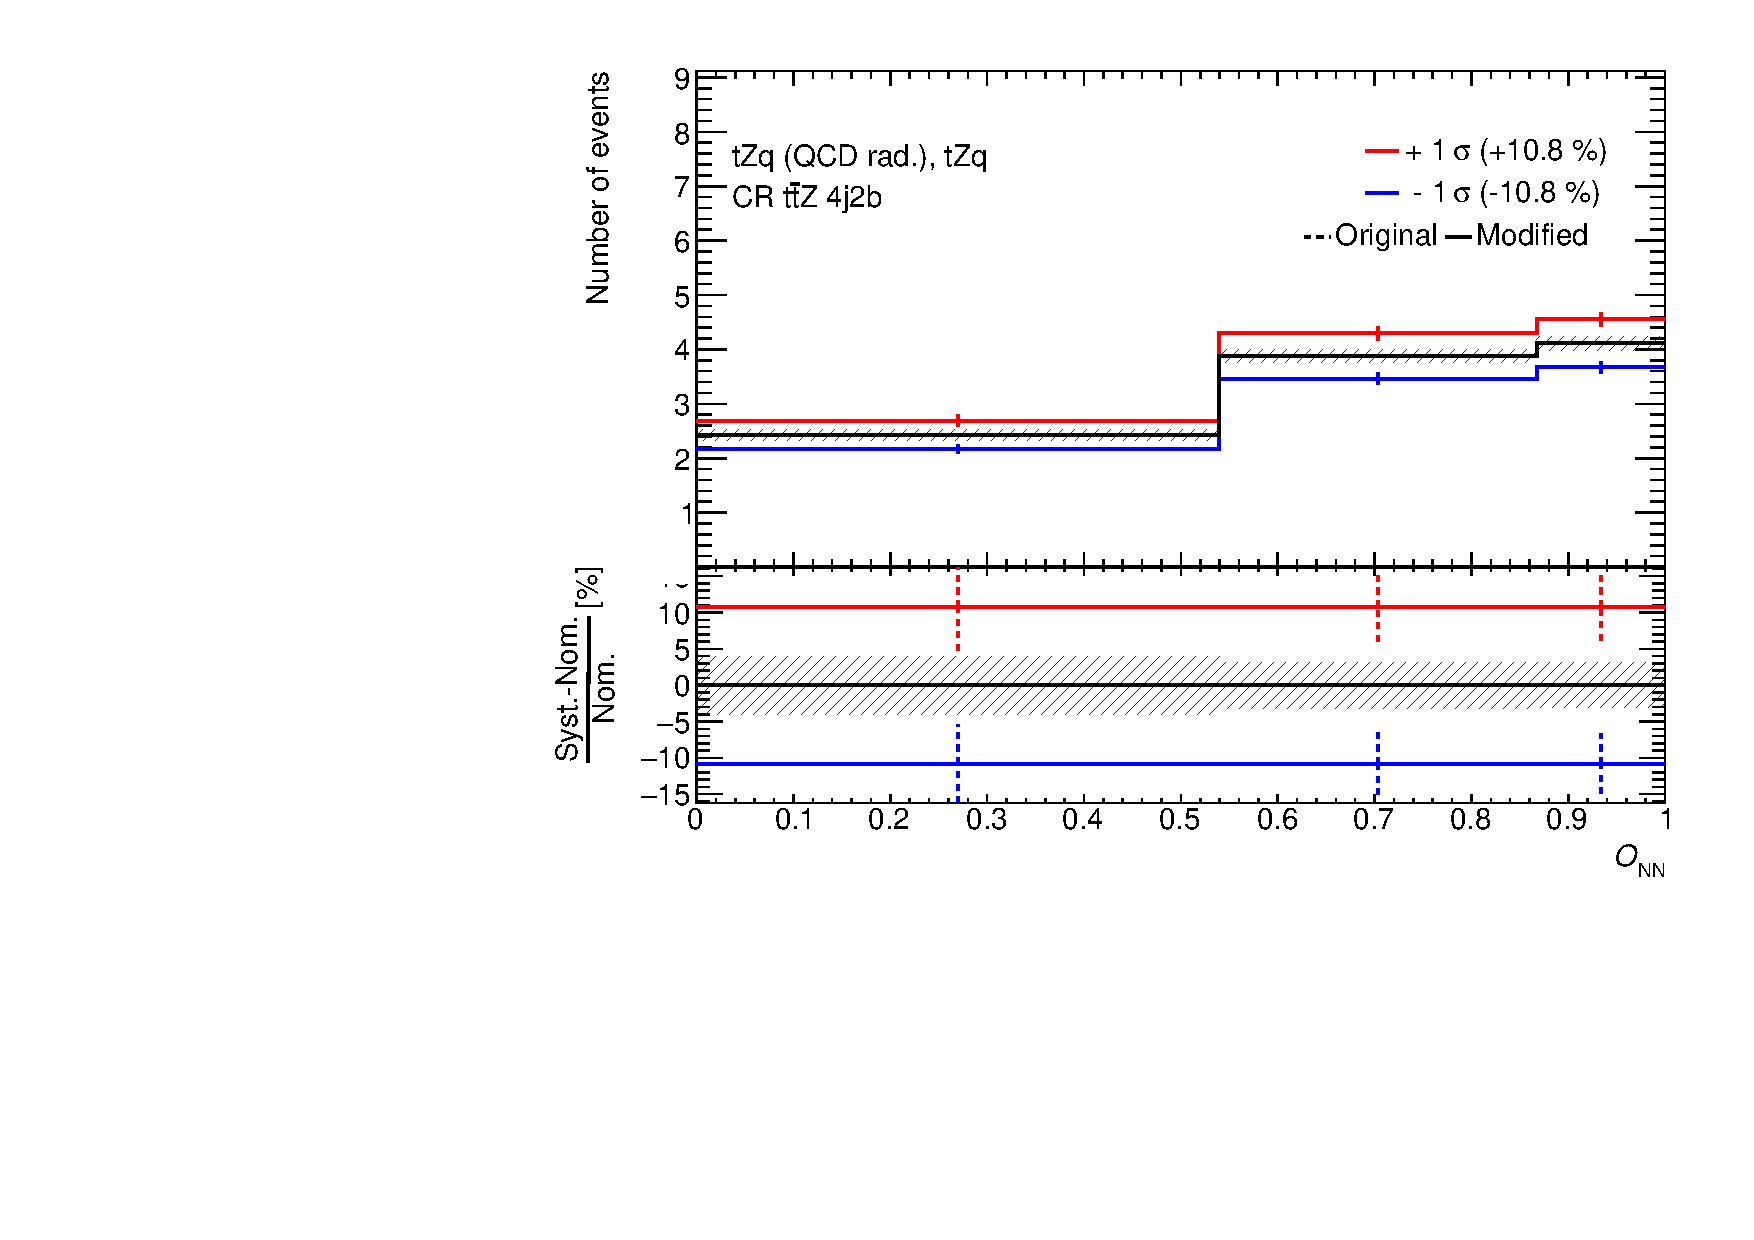
\includegraphics[width=\textwidth]{ubonn-thesis/Chapters/Chapters_07/Figure/Data/Systematic/tZq_qcdrad/CR_4j2b_tZq_tZq_XS_QCDscale.pdf} 
    \caption{}
  \end{subfigure} 
  \begin{subfigure}[b]{0.33\linewidth}
  \centering
    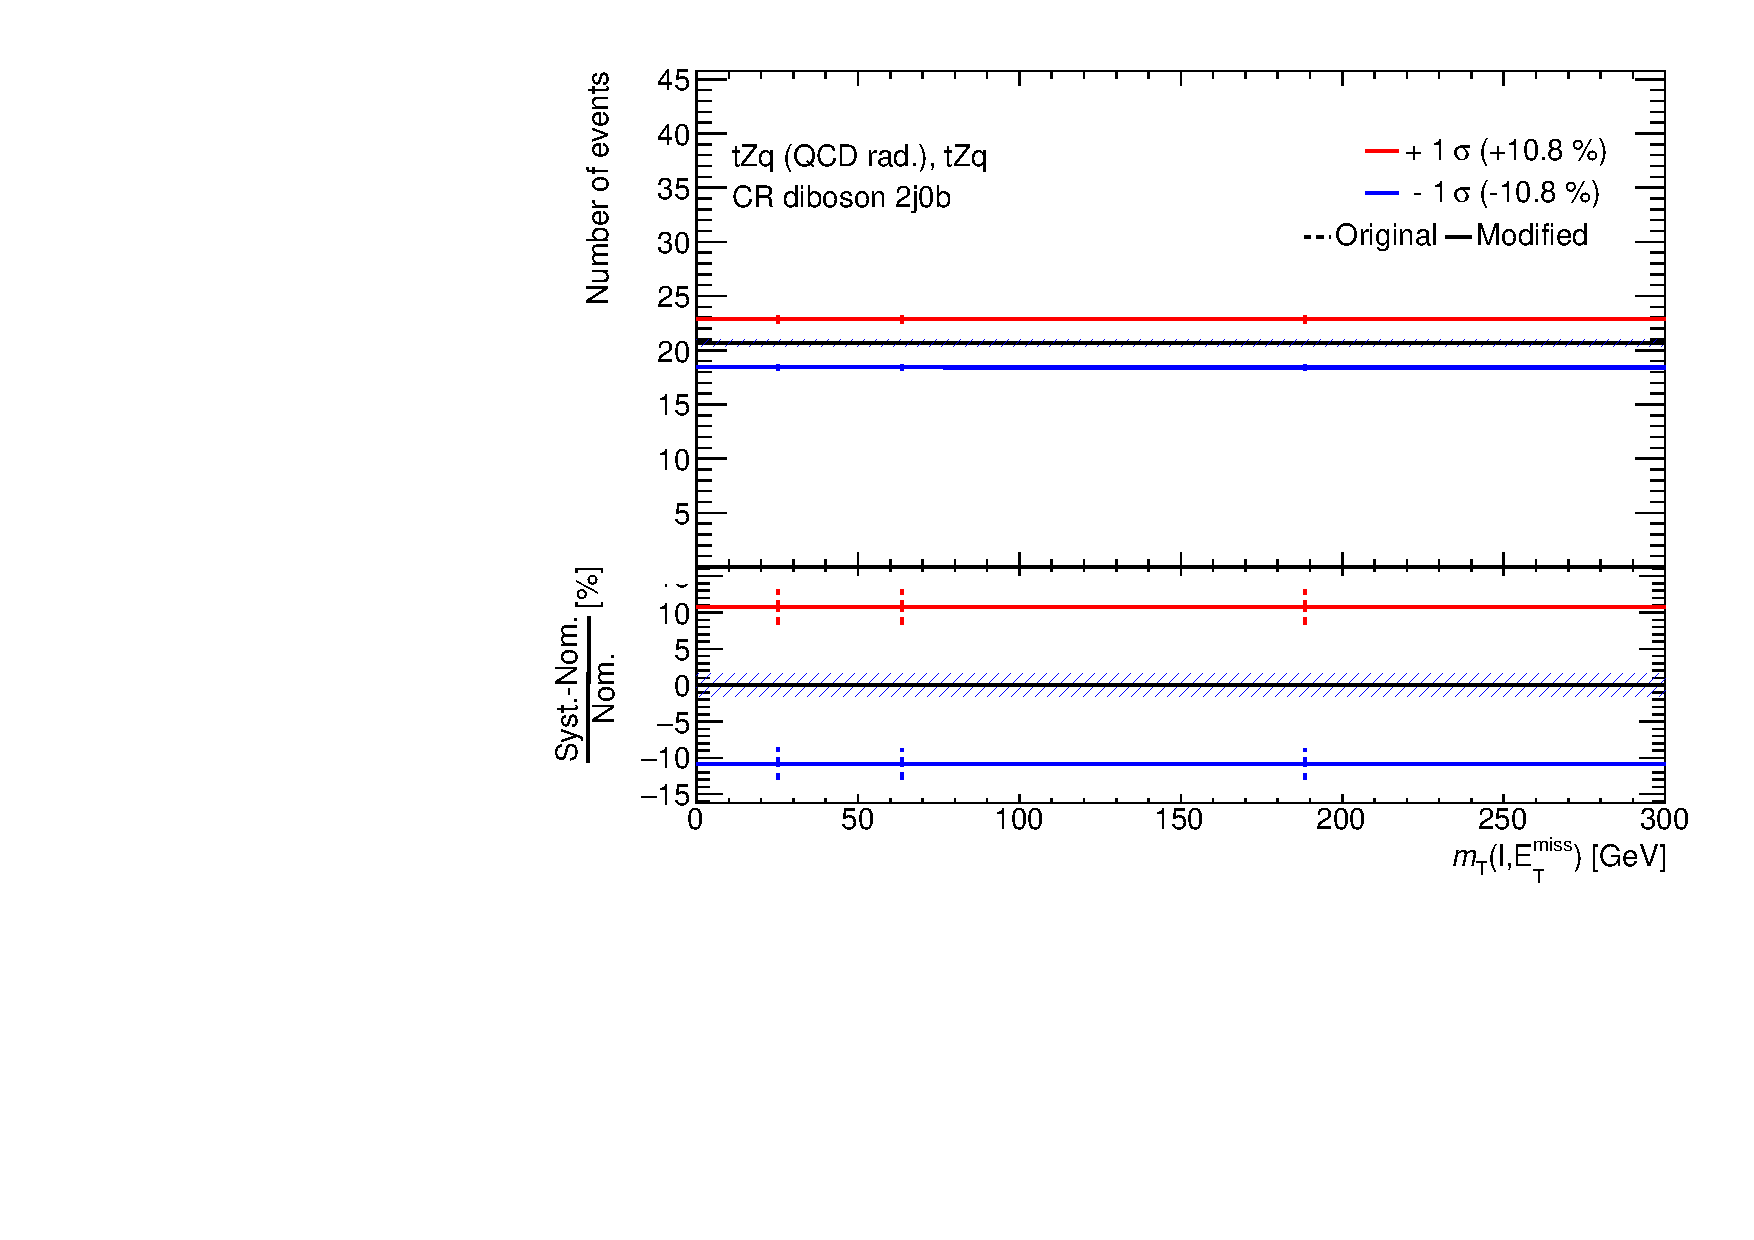
\includegraphics[width=\textwidth]{ubonn-thesis/Chapters/Chapters_07/Figure/Data/Systematic/tZq_qcdrad/CR_2j0b_tZq_tZq_XS_QCDscale.pdf} 
    \caption{}
  \end{subfigure}%% 
   \begin{subfigure}[b]{0.33\linewidth}
  \centering
    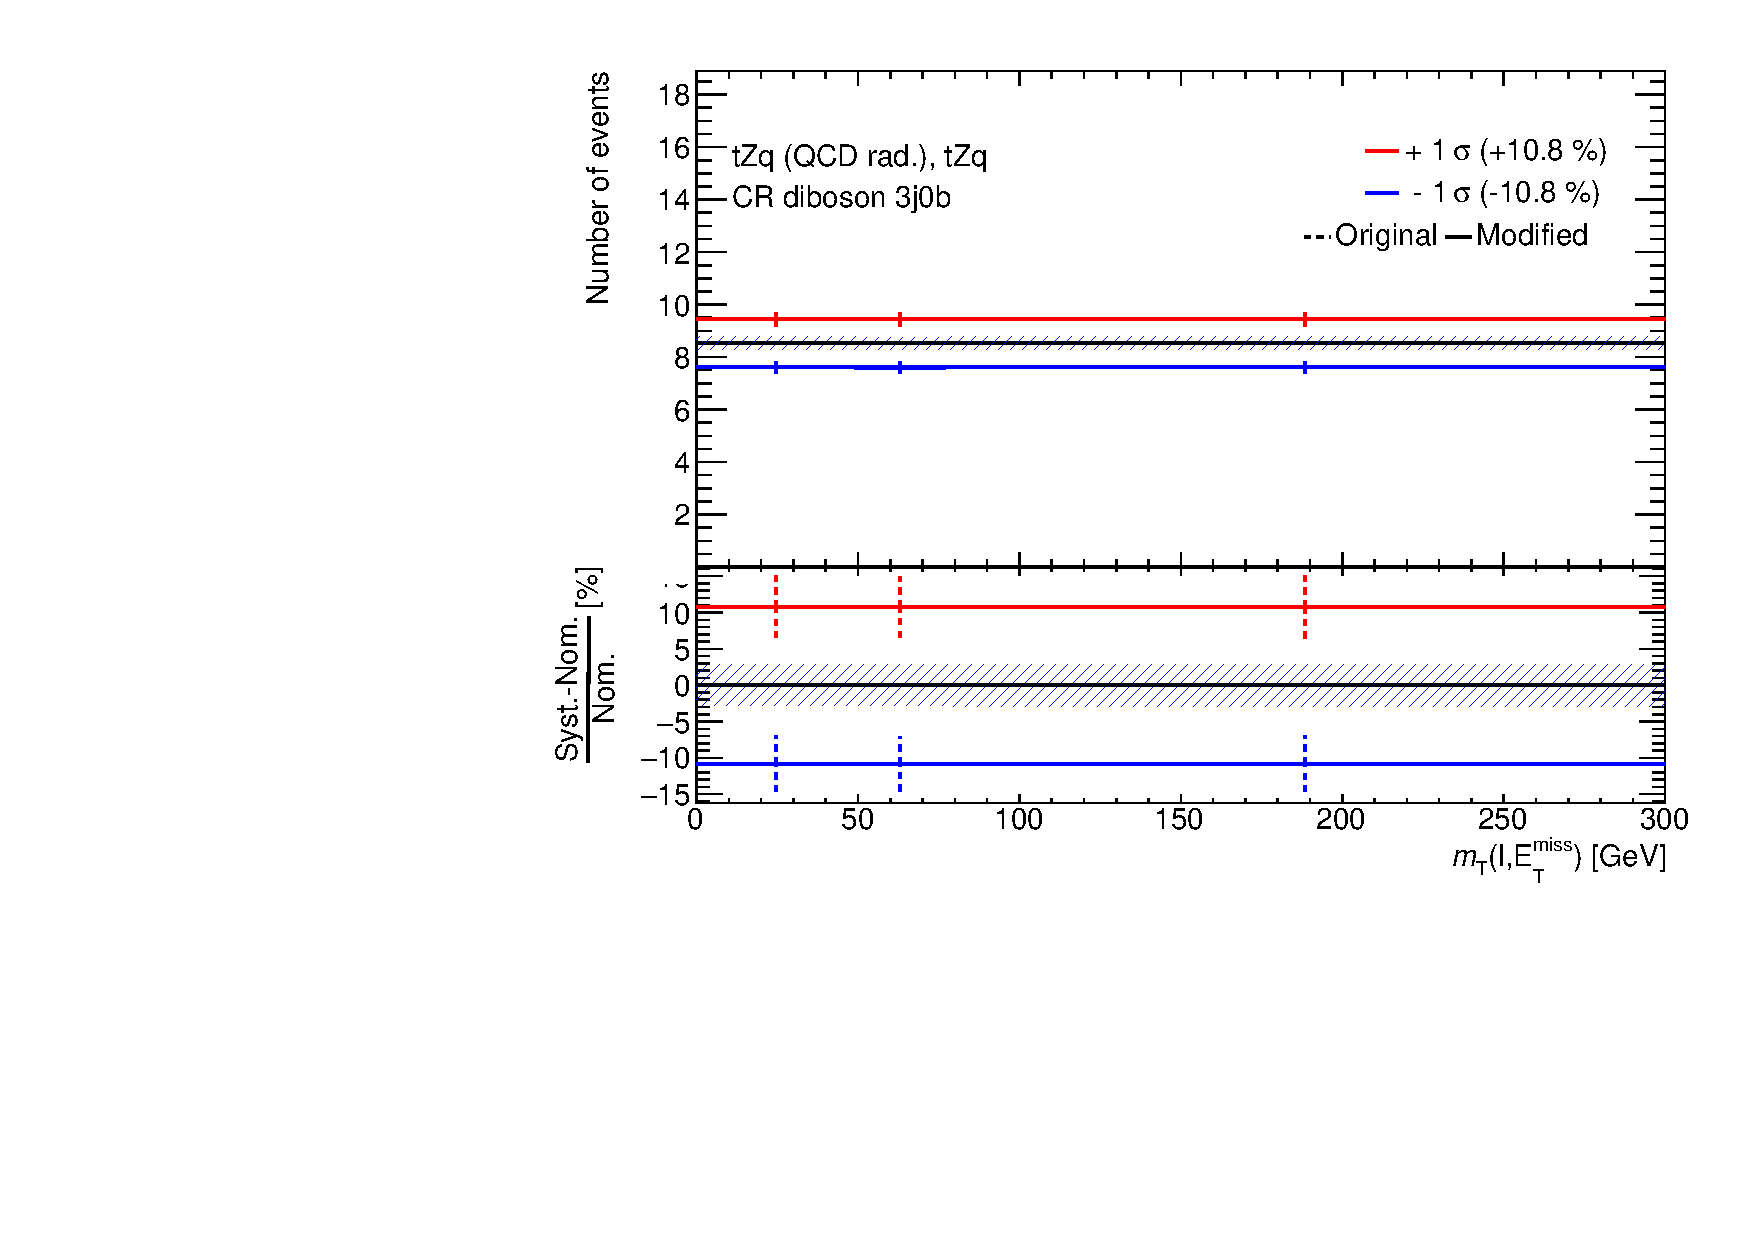
\includegraphics[width=\textwidth]{ubonn-thesis/Chapters/Chapters_07/Figure/Data/Systematic/tZq_qcdrad/CR_3j0b_tZq_tZq_XS_QCDscale.pdf} 
    \caption{}
  \end{subfigure}%% 
  \newline
  \centering
  \begin{subfigure}[b]{0.33\linewidth}
  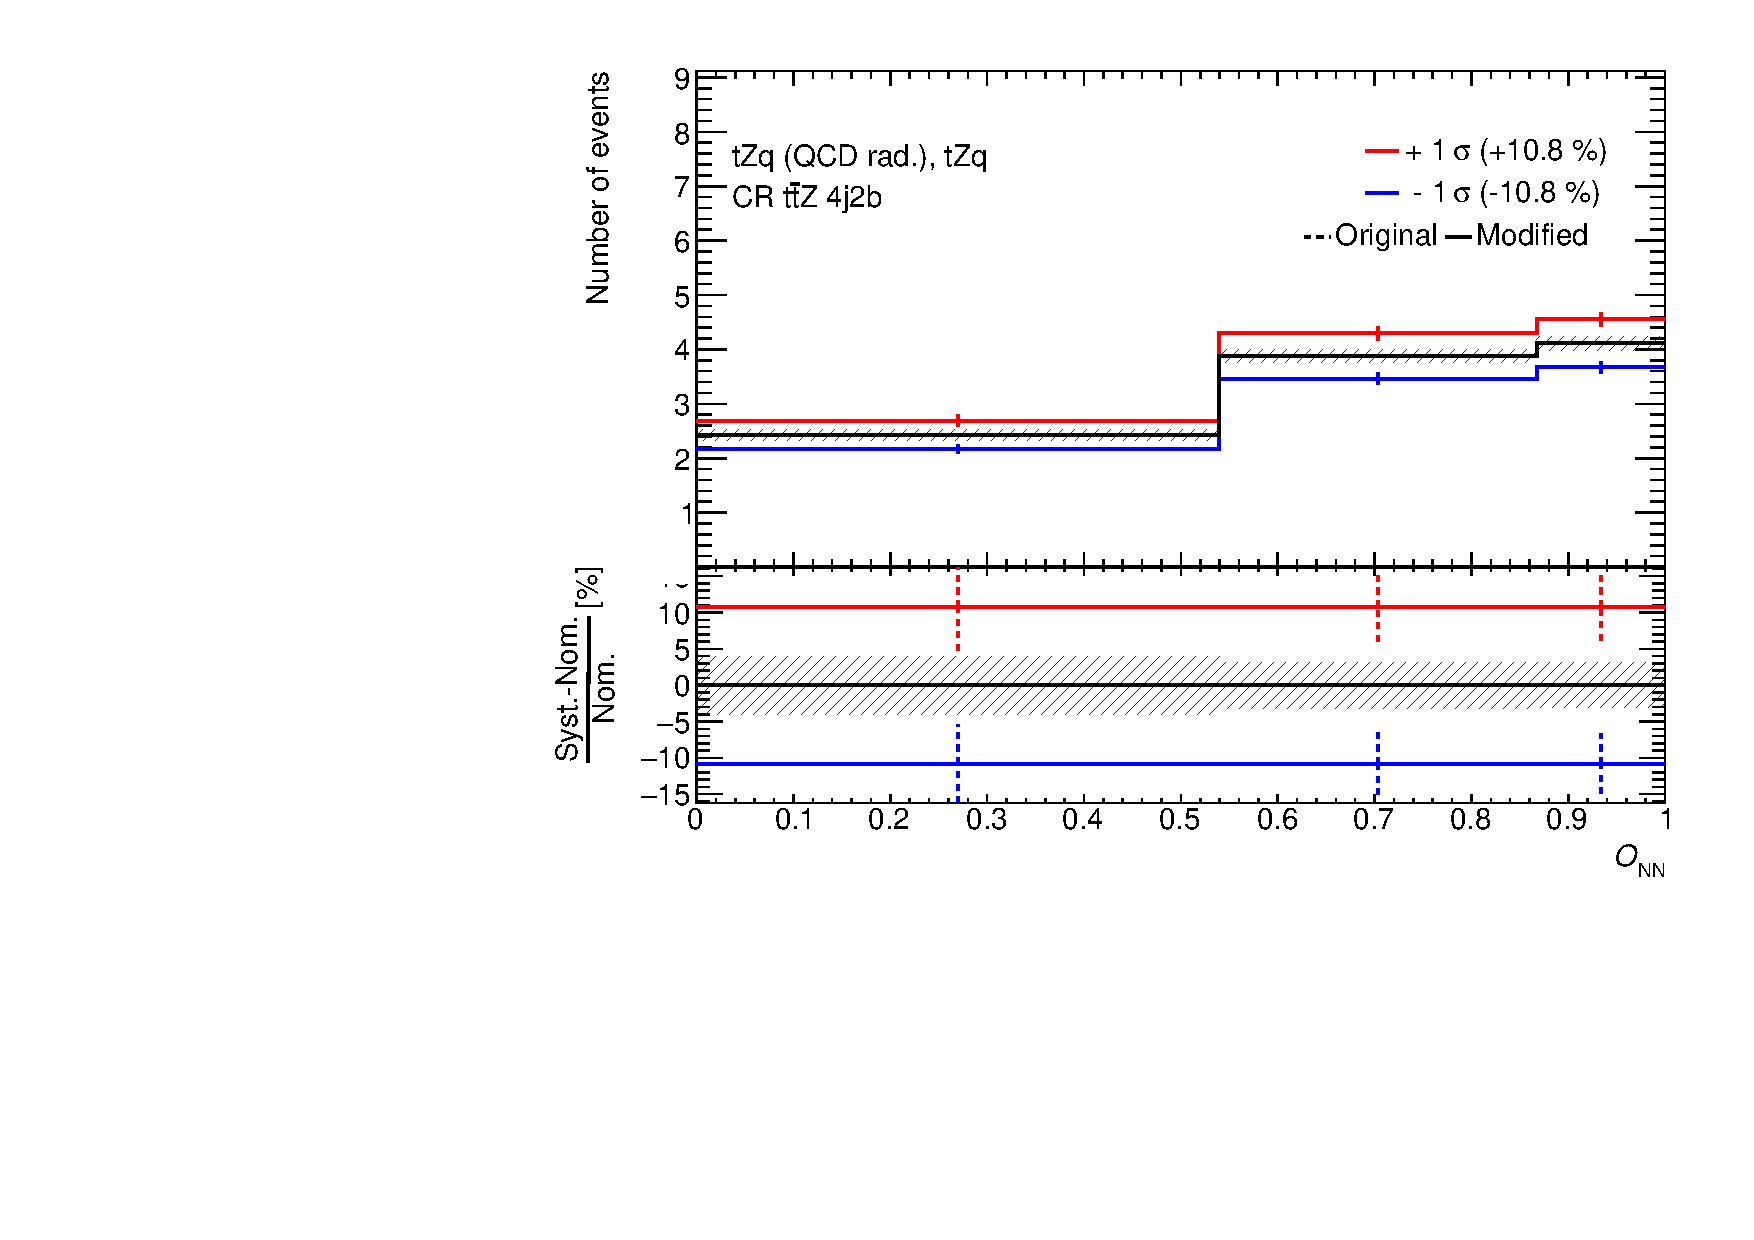
\includegraphics[width=\textwidth]{ubonn-thesis/Chapters/Chapters_07/Figure/Data/Systematic/tZq_qcdrad/CR_4j2b_tZq_tZq_XS_QCDscale.pdf} 
    \caption{}
  \end{subfigure} 
  \centering
  \begin{subfigure}[b]{0.33\linewidth}
    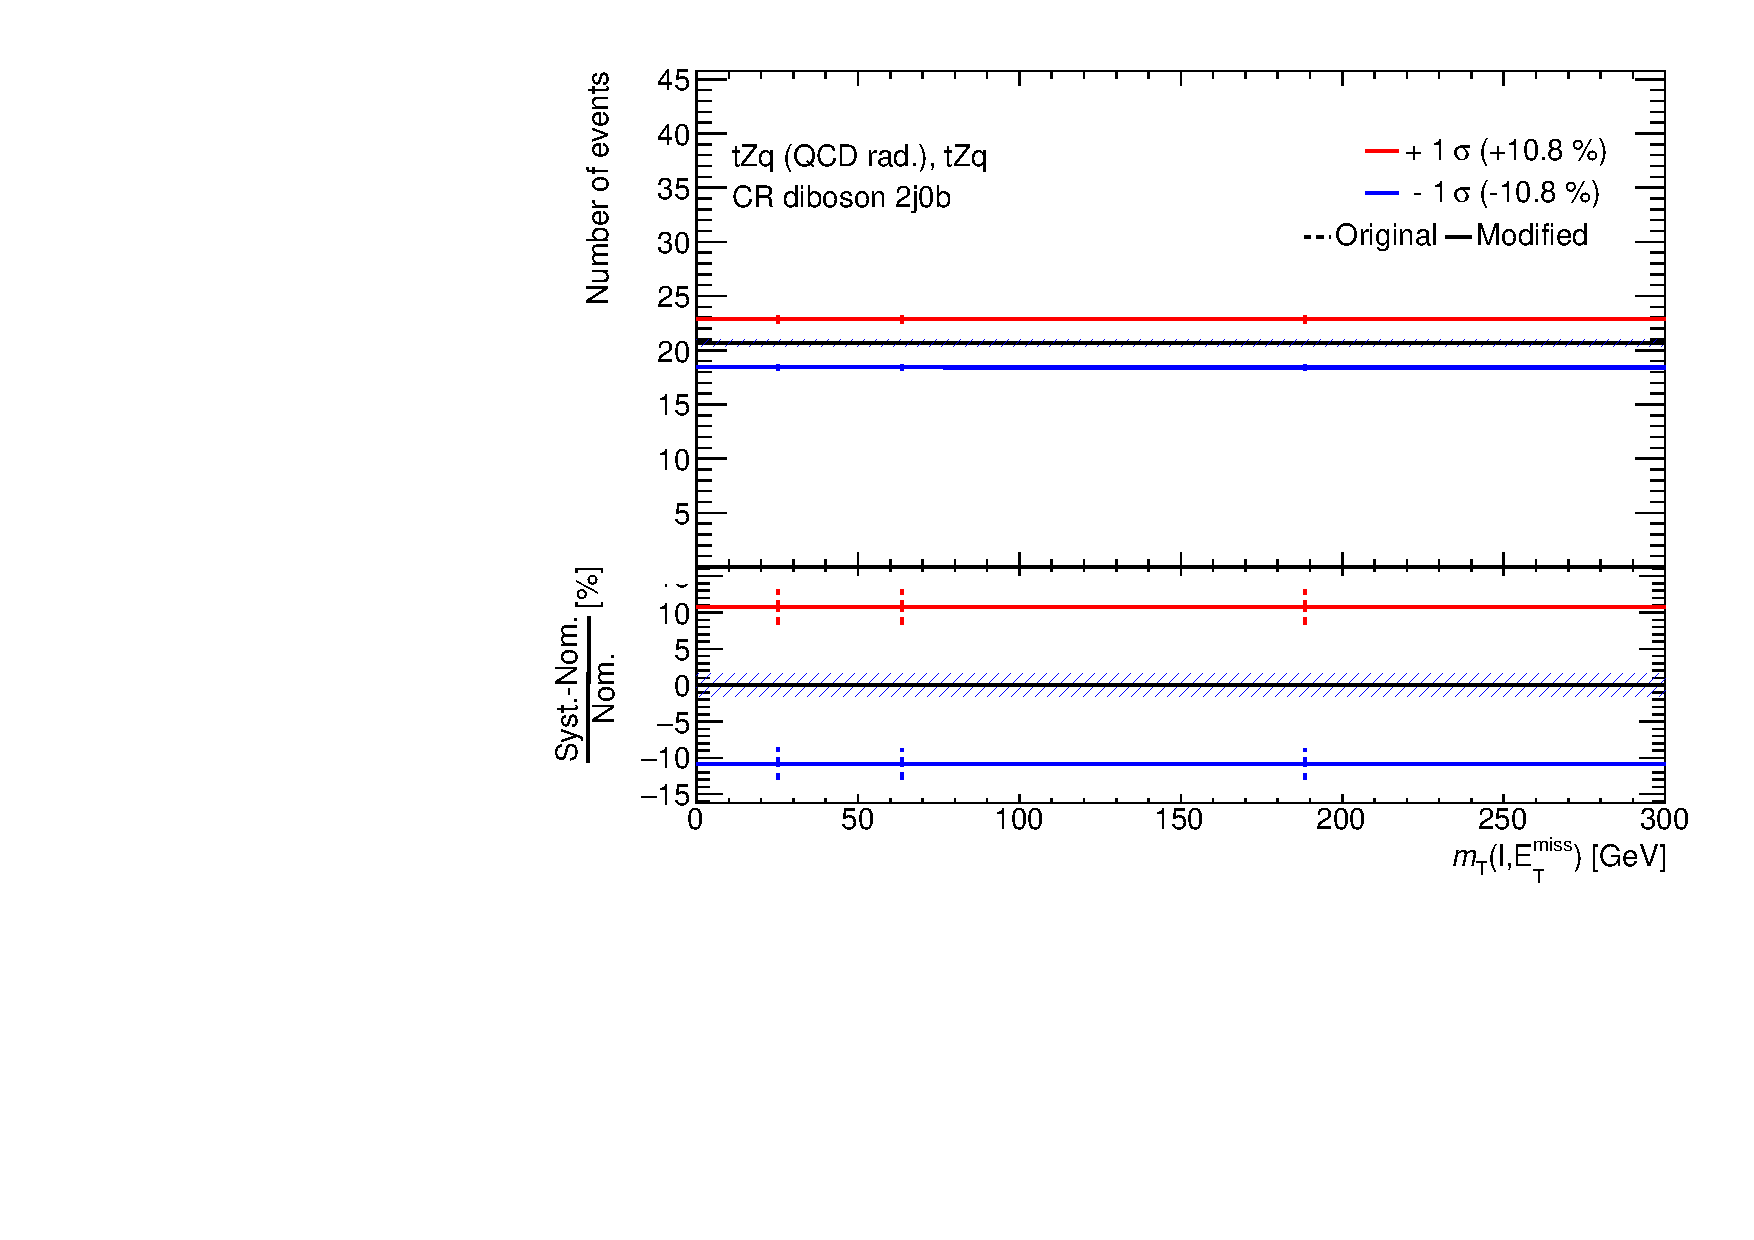
\includegraphics[width=\textwidth]{ubonn-thesis/Chapters/Chapters_07/Figure/Data/Systematic/tZq_qcdrad/CR_2j0b_tZq_tZq_XS_QCDscale.pdf} 
    \caption{}
  \end{subfigure}
  \caption{ The effects of the tZq QCD rad. on the total prediction in the signal and control regions. Here, lines coloured in red/blue present the $\pm 1 \sigma$ effect. The dotted/solid lines show the effect before/after smoothing, symmetrisation, and the removal of the normalisation effect (only done for shape uncertainties). The hashed bands represent the MC statistical uncertainties.}
  \label{fig:systQCD}
  \end{figure}


%% tZ pdf systematics

  
\setcounter{figure}{11} 
\begin{figure}[!h] 
 \begin{subfigure}[b]{0.33\linewidth}
    \centering
    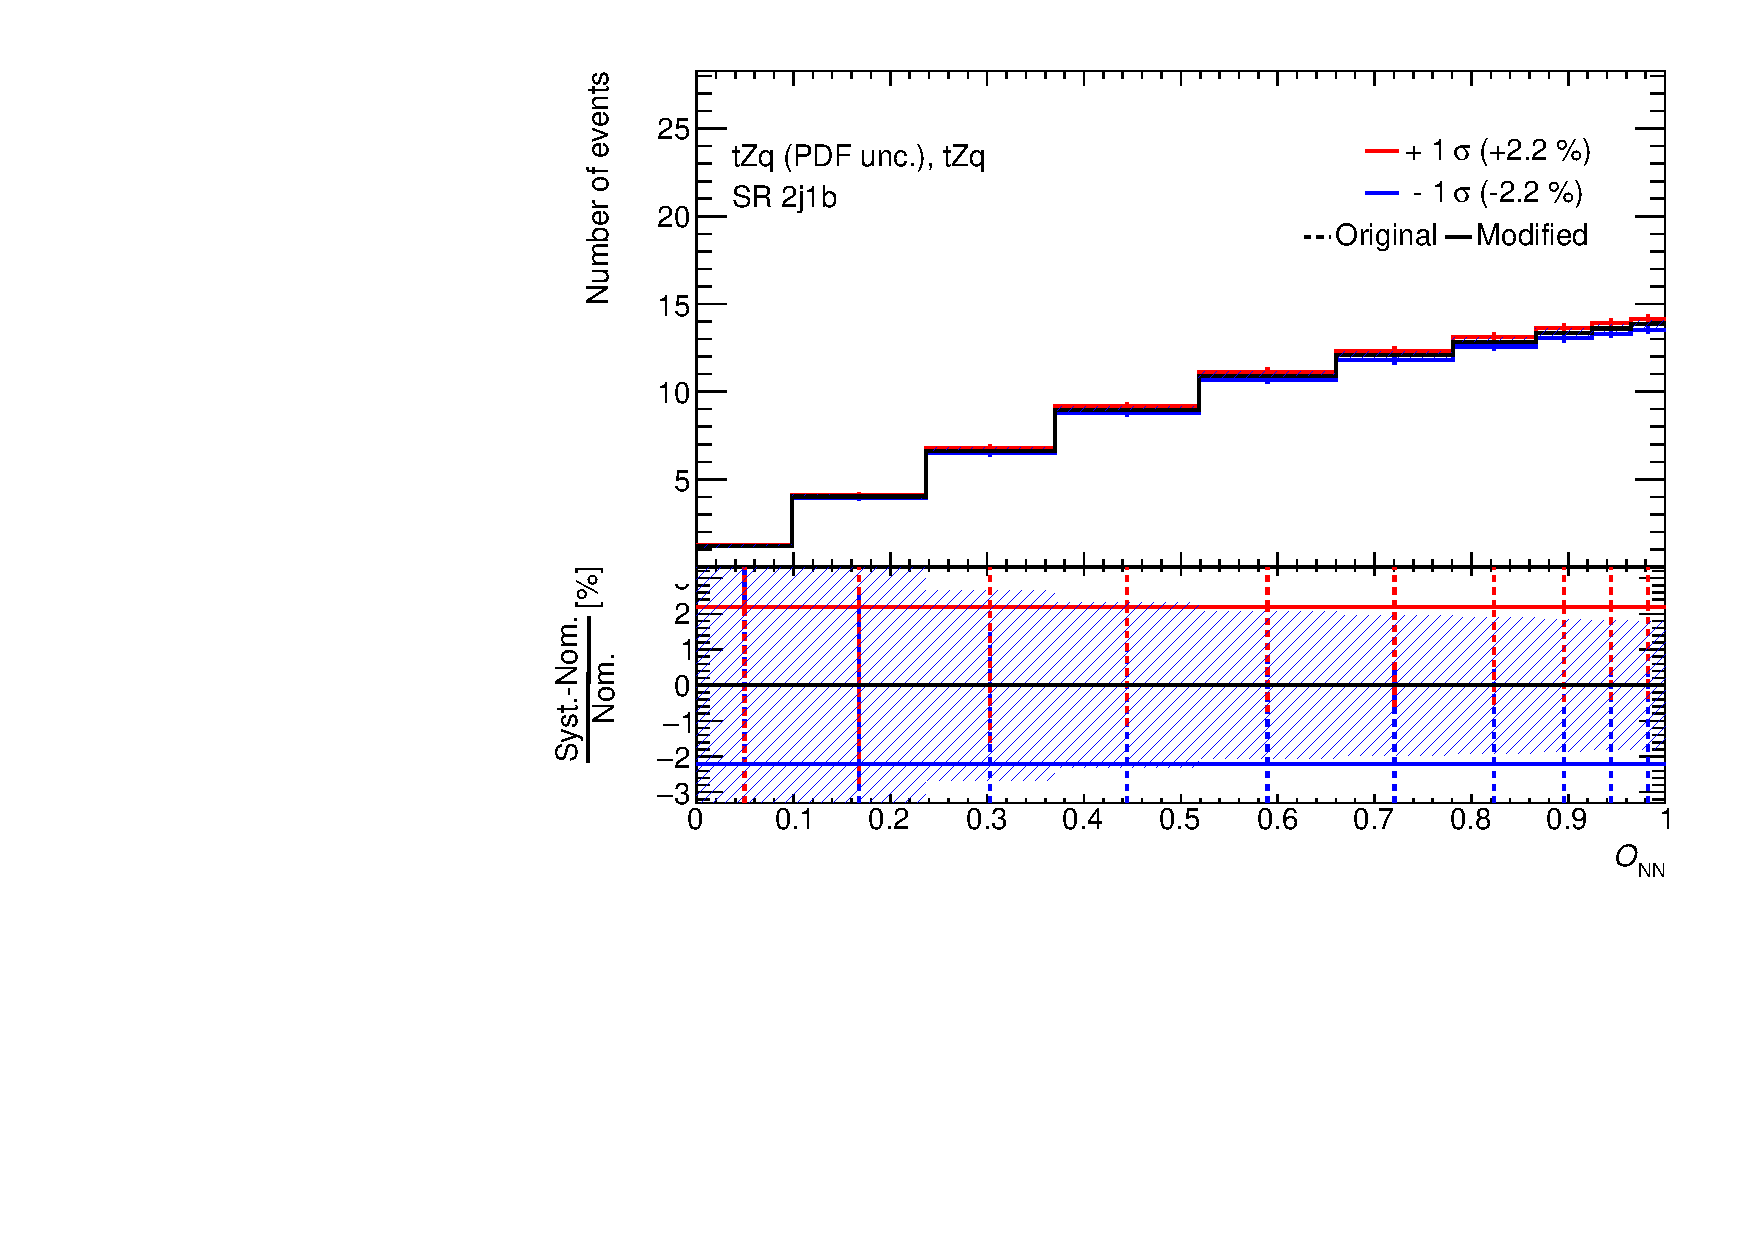
\includegraphics[width=\textwidth]{ubonn-thesis/Chapters/Chapters_07/Figure/Data/Systematic/tZq_pdf/SR_2j1b_tZq_tZq_XS_PDFunc.pdf} 
    \caption{}
  \end{subfigure}%% 
  \begin{subfigure}[b]{0.33\linewidth}
    \centering
    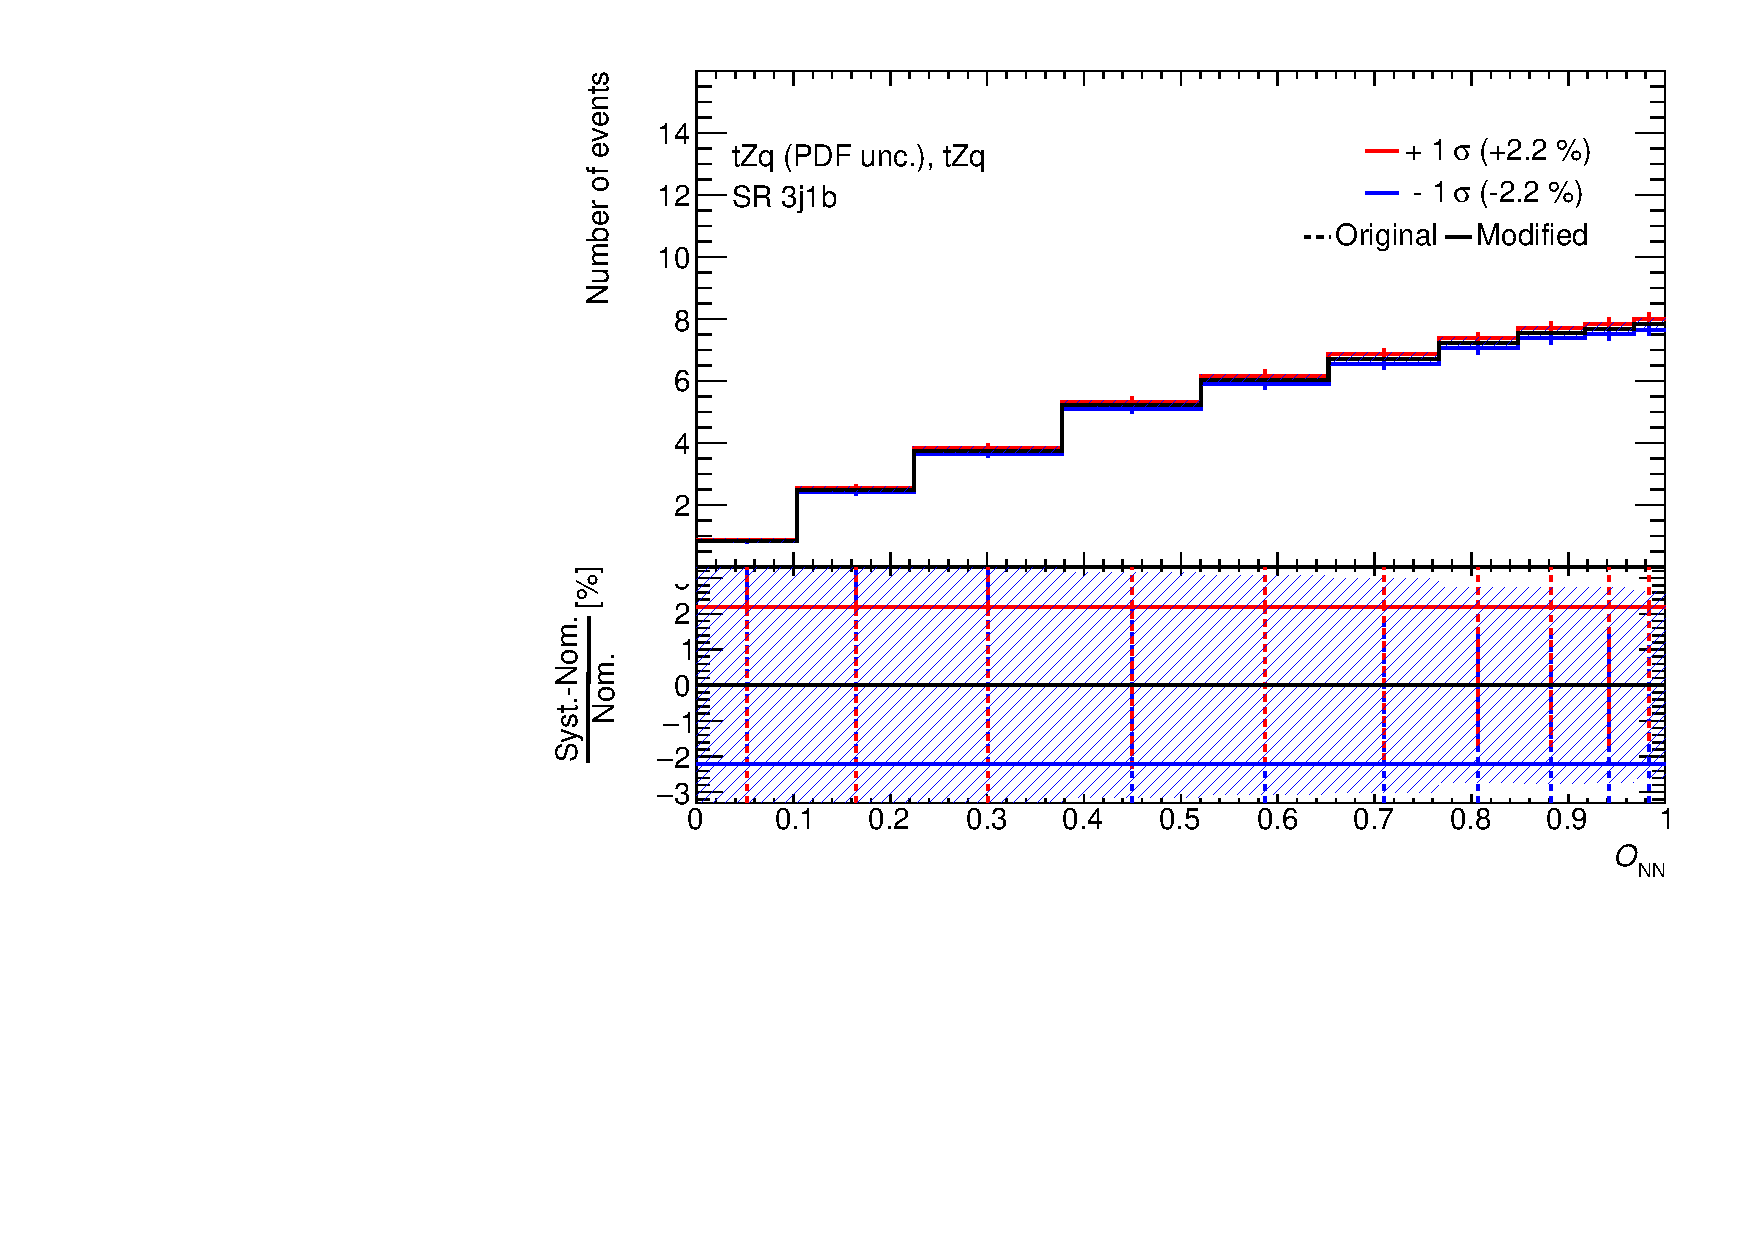
\includegraphics[width=\textwidth]{ubonn-thesis/Chapters/Chapters_07/Figure/Data/Systematic/tZq_pdf/SR_3j1b_tZq_tZq_XS_PDFunc.pdf} 
    \caption{}
  \end{subfigure} 
  \begin{subfigure}[b]{0.33\linewidth}
    \centering
    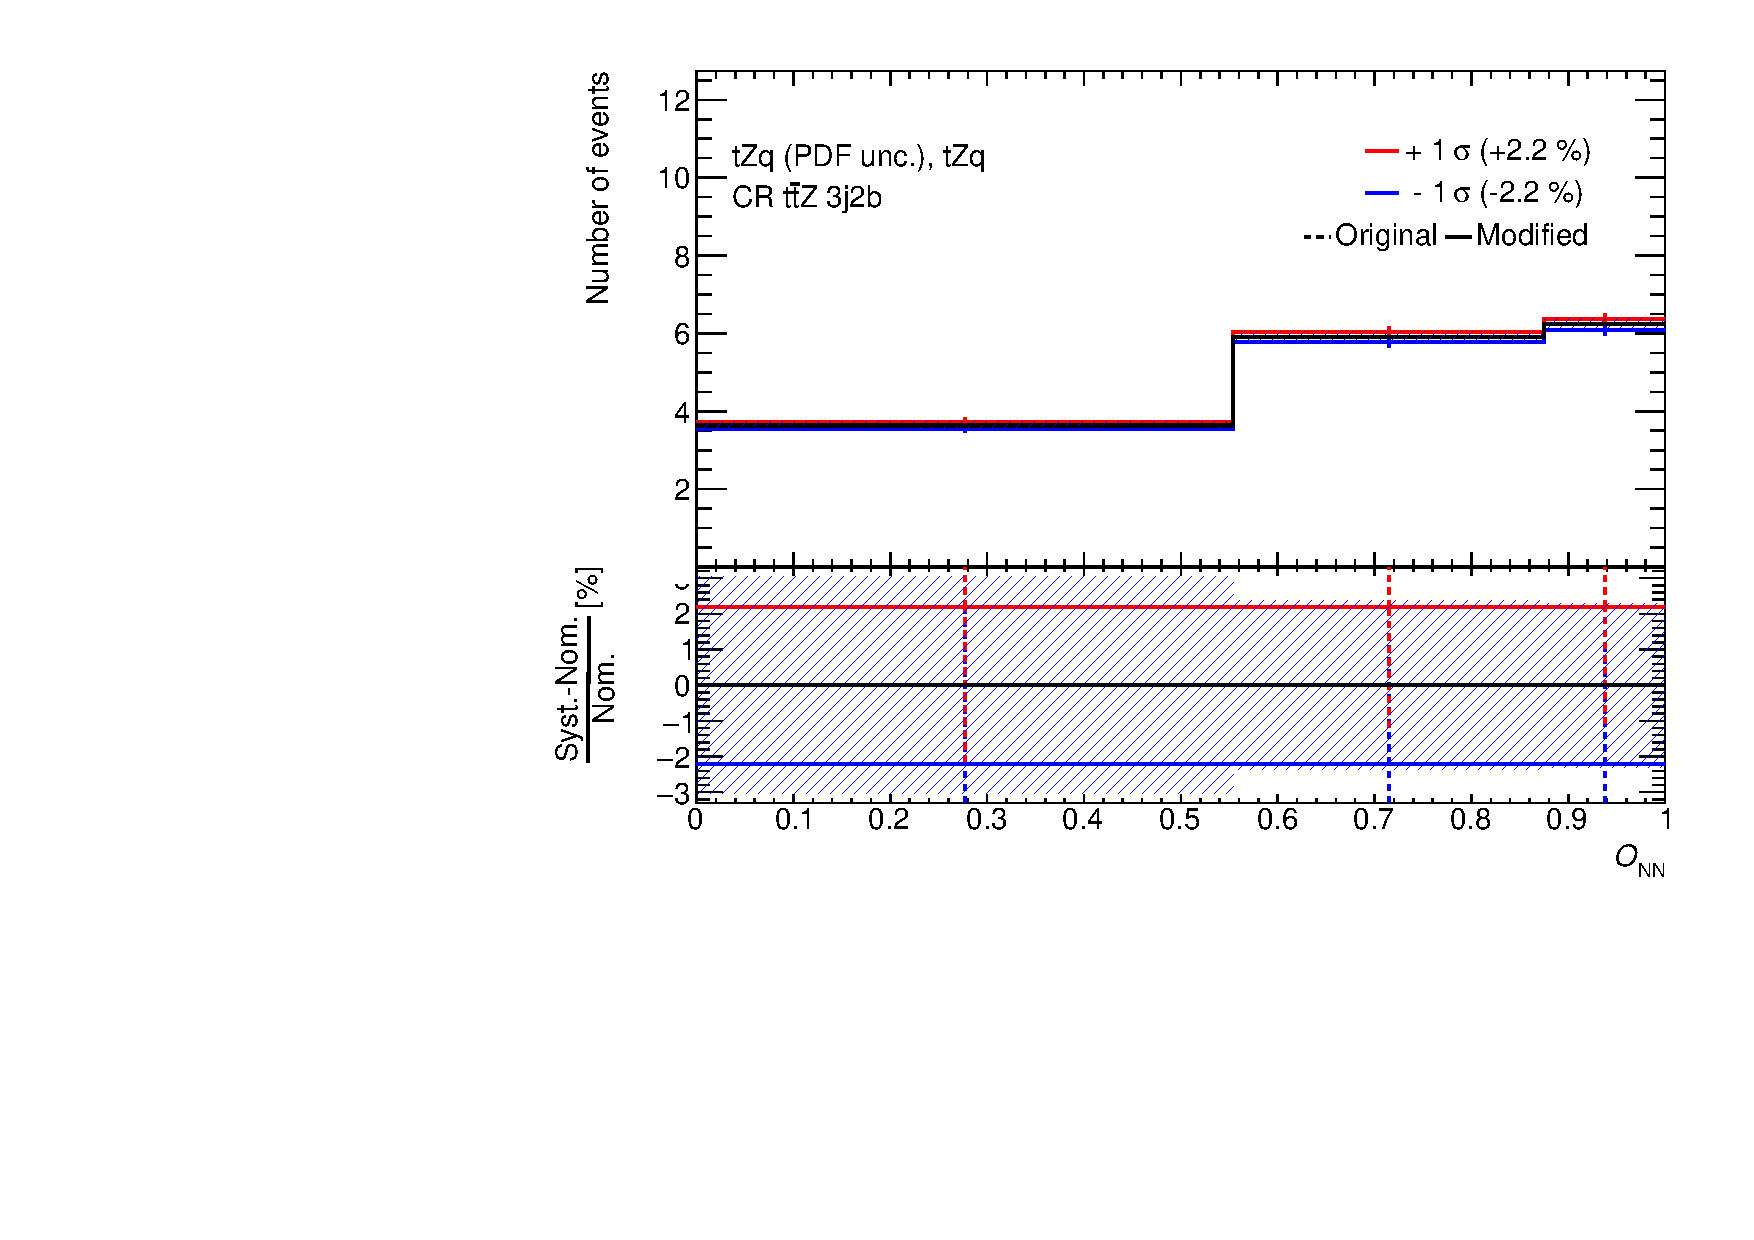
\includegraphics[width=\textwidth]{ubonn-thesis/Chapters/Chapters_07/Figure/Data/Systematic/tZq_pdf/CR_3j2b_tZq_tZq_XS_PDFunc.pdf} 
    \caption{}
  \end{subfigure}%%
  \newline
  \begin{subfigure}[b]{0.33\linewidth}
  \centering
    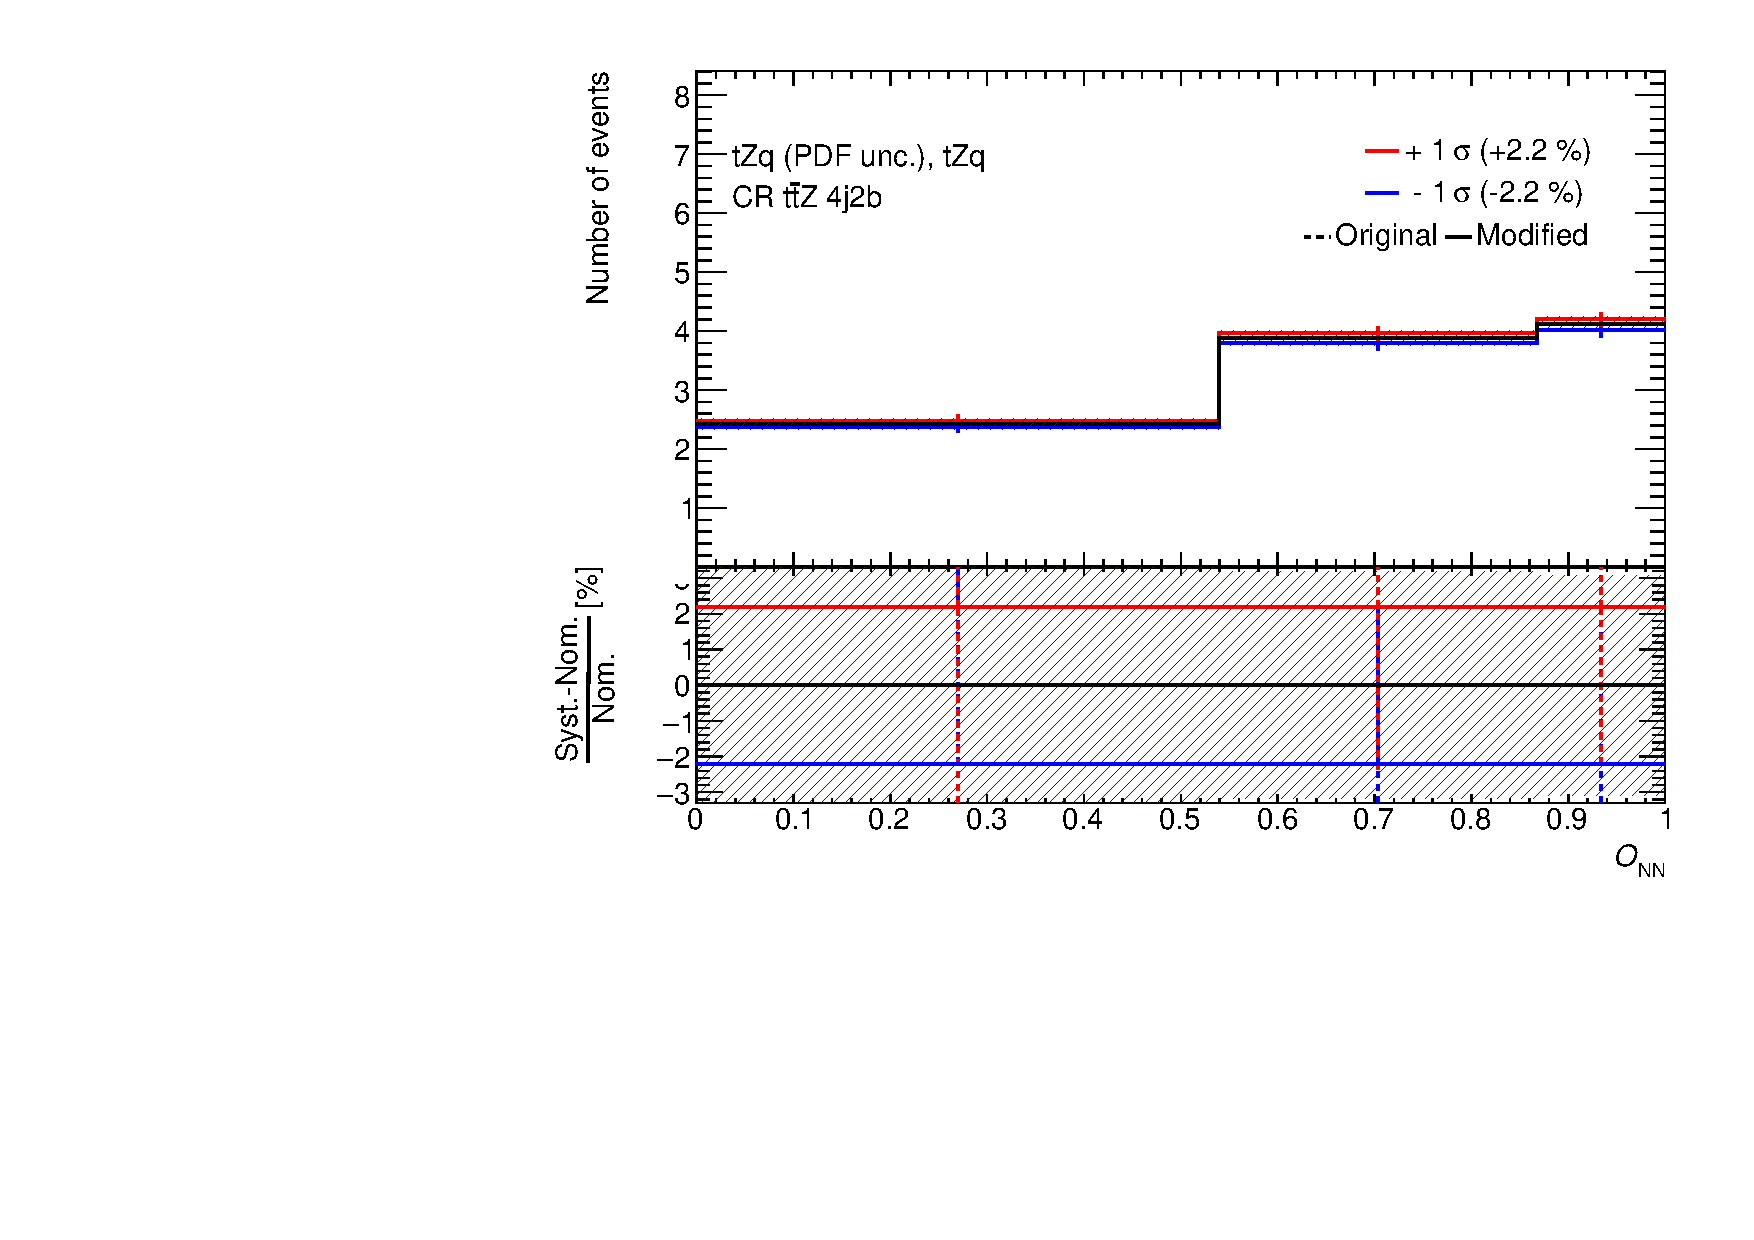
\includegraphics[width=\textwidth]{ubonn-thesis/Chapters/Chapters_07/Figure/Data/Systematic/tZq_pdf/CR_4j2b_tZq_tZq_XS_PDFunc.pdf} 
    \caption*{(d)}
  \end{subfigure} 
  \begin{subfigure}[b]{0.33\linewidth}
  \centering
    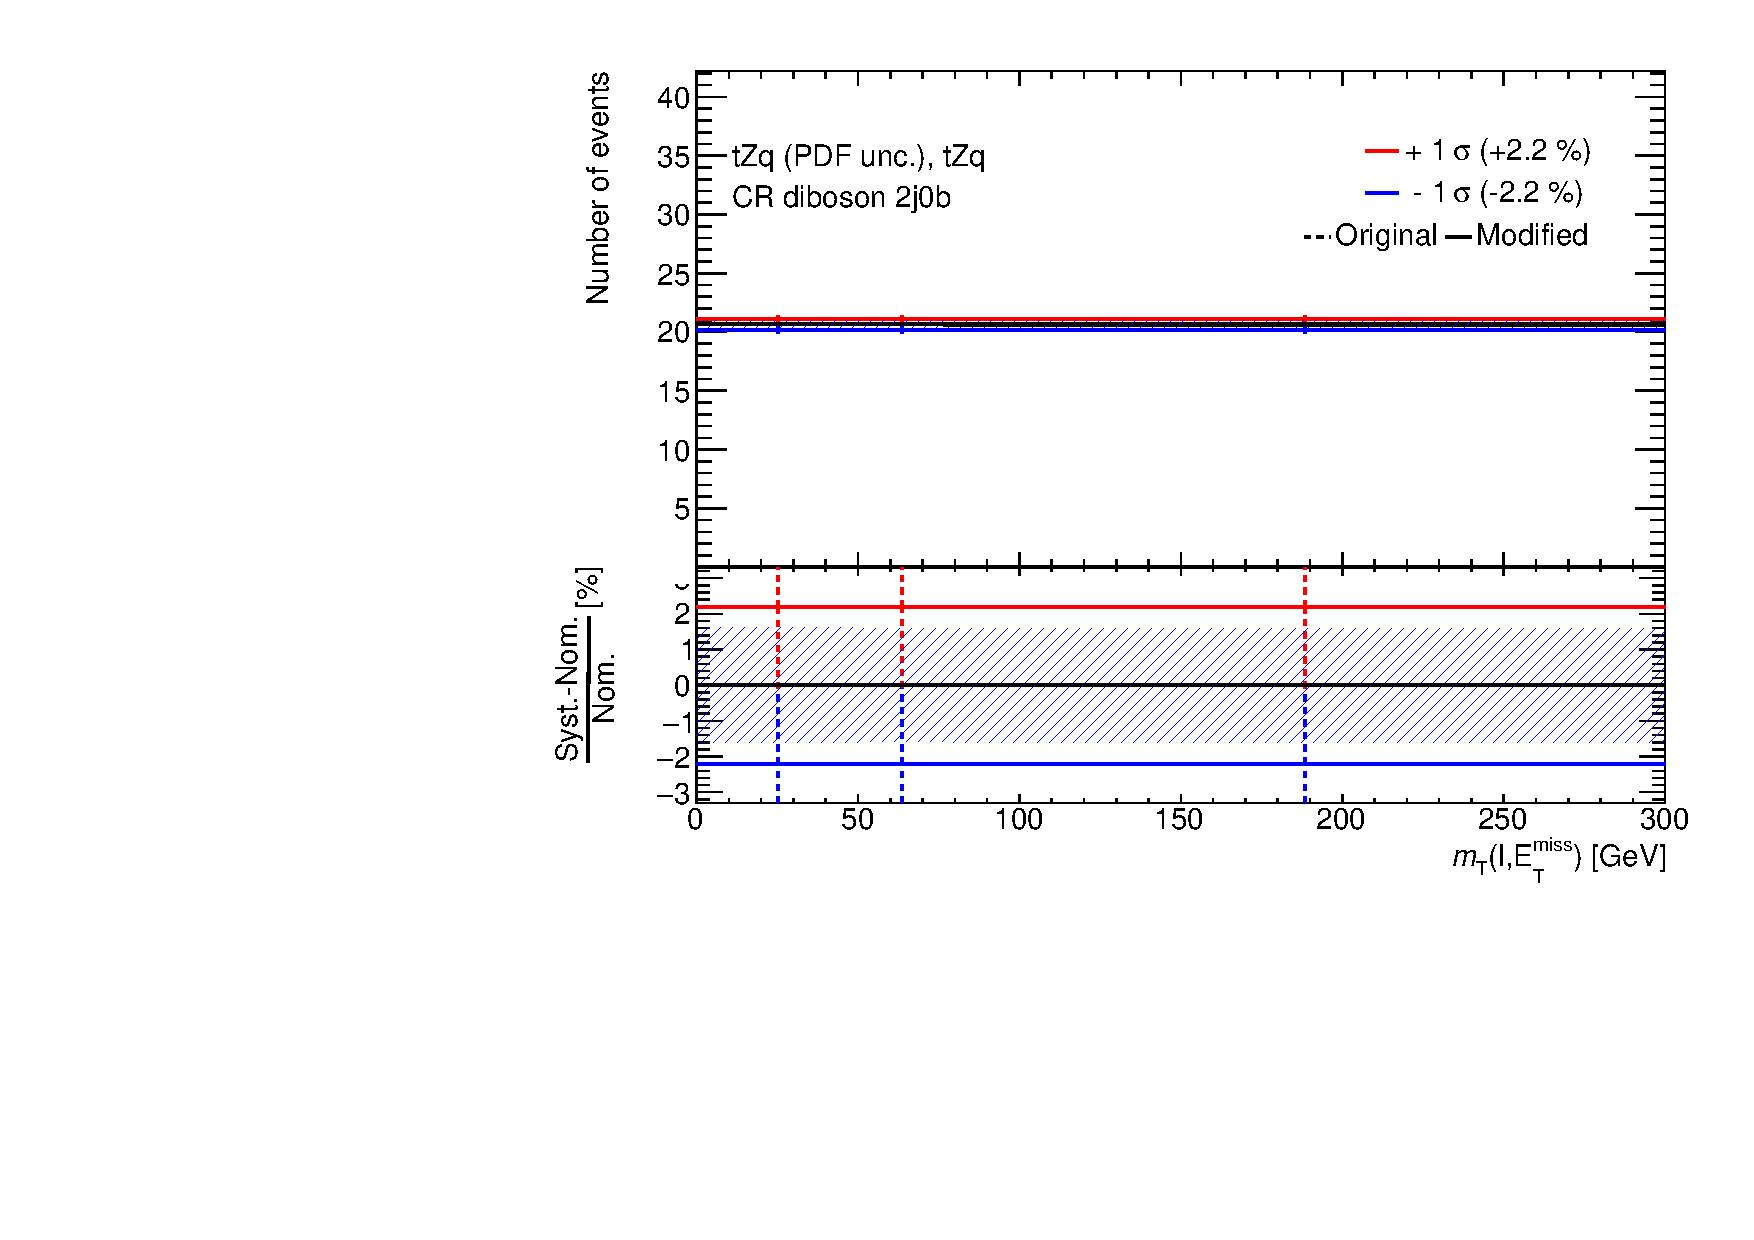
\includegraphics[width=\textwidth]{ubonn-thesis/Chapters/Chapters_07/Figure/Data/Systematic/tZq_pdf/CR_2j0b_tZq_tZq_XS_PDFunc.pdf} 
    \caption*{(e)}
  \end{subfigure}%% 
   \begin{subfigure}[b]{0.33\linewidth}
  \centering
    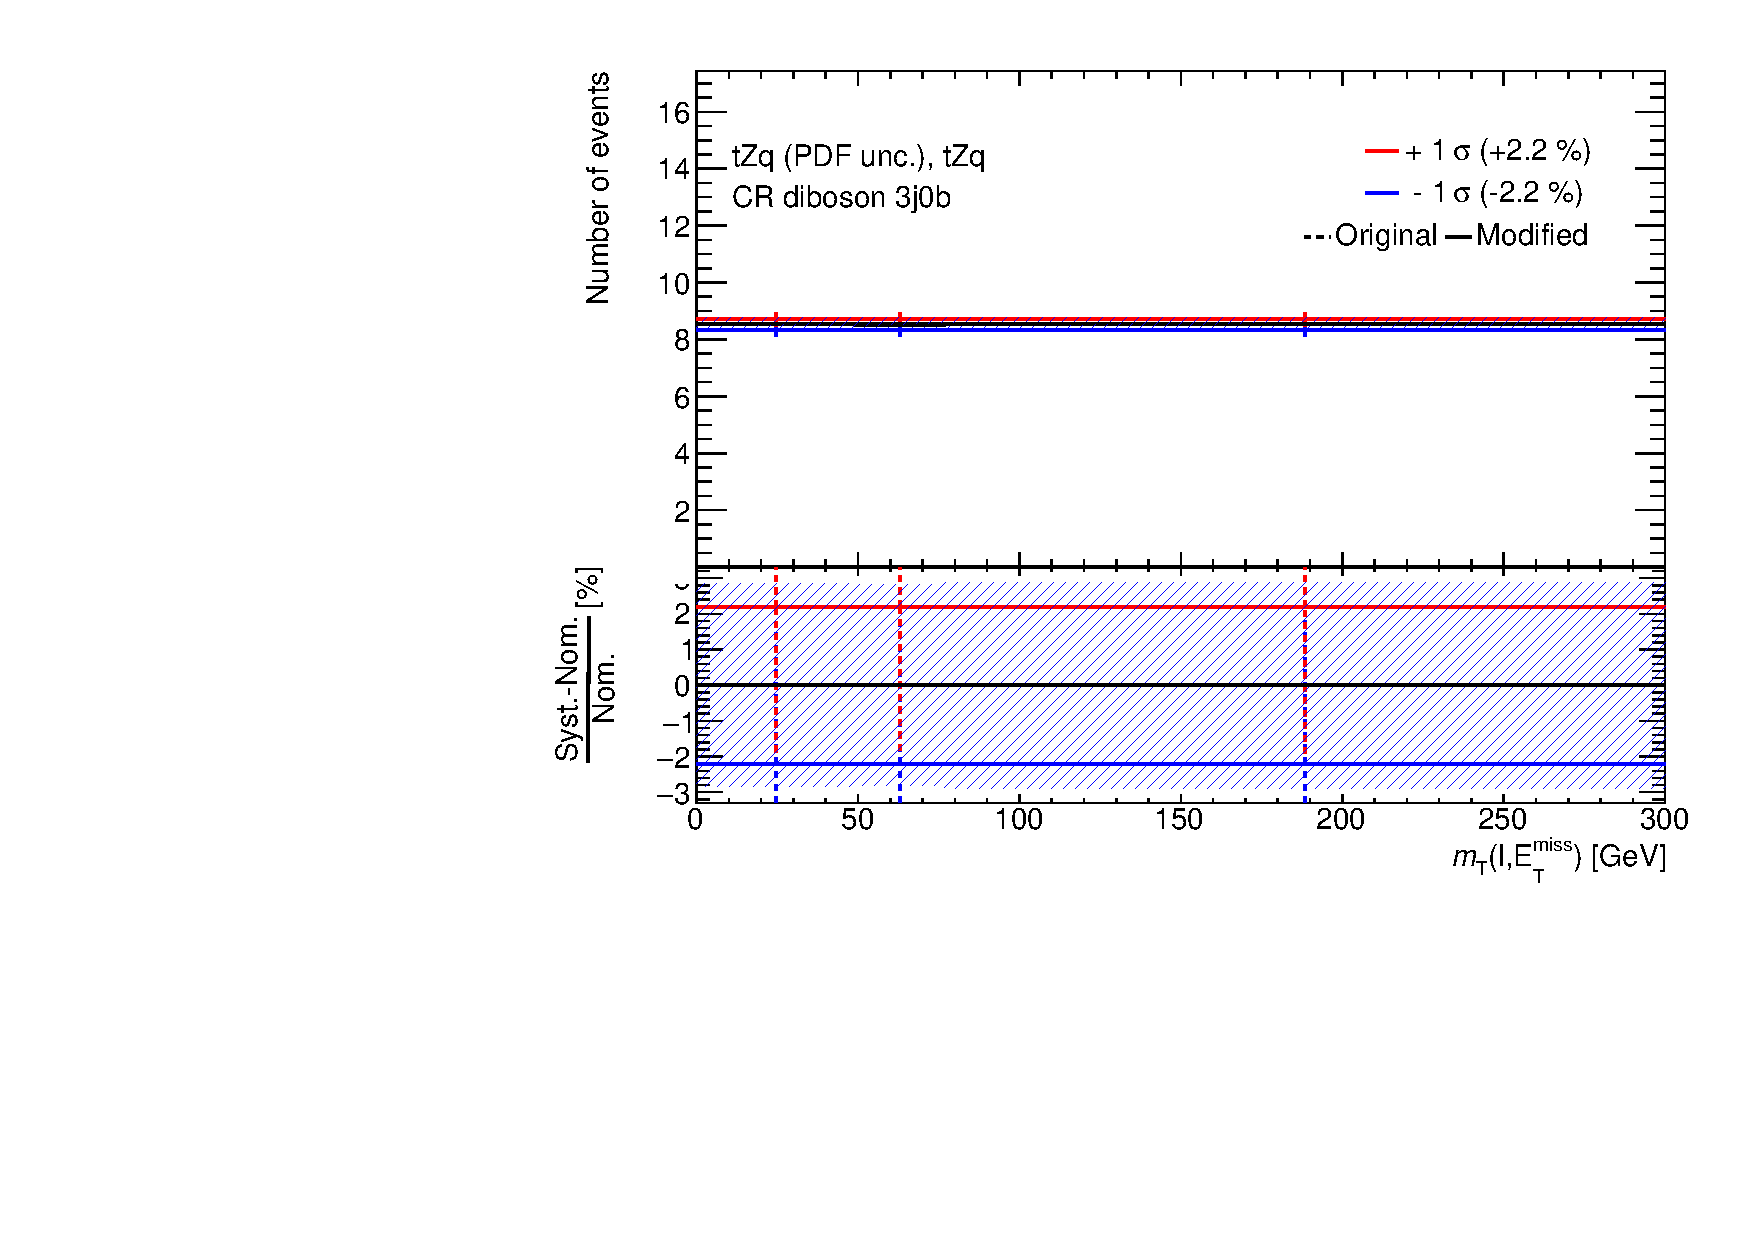
\includegraphics[width=\textwidth]{ubonn-thesis/Chapters/Chapters_07/Figure/Data/Systematic/tZq_pdf/CR_3j0b_tZq_tZq_XS_PDFunc.pdf} 
    \caption*{(f)}
  \end{subfigure}%% 
  \newline
  \centering
  \begin{subfigure}[b]{0.33\linewidth}
  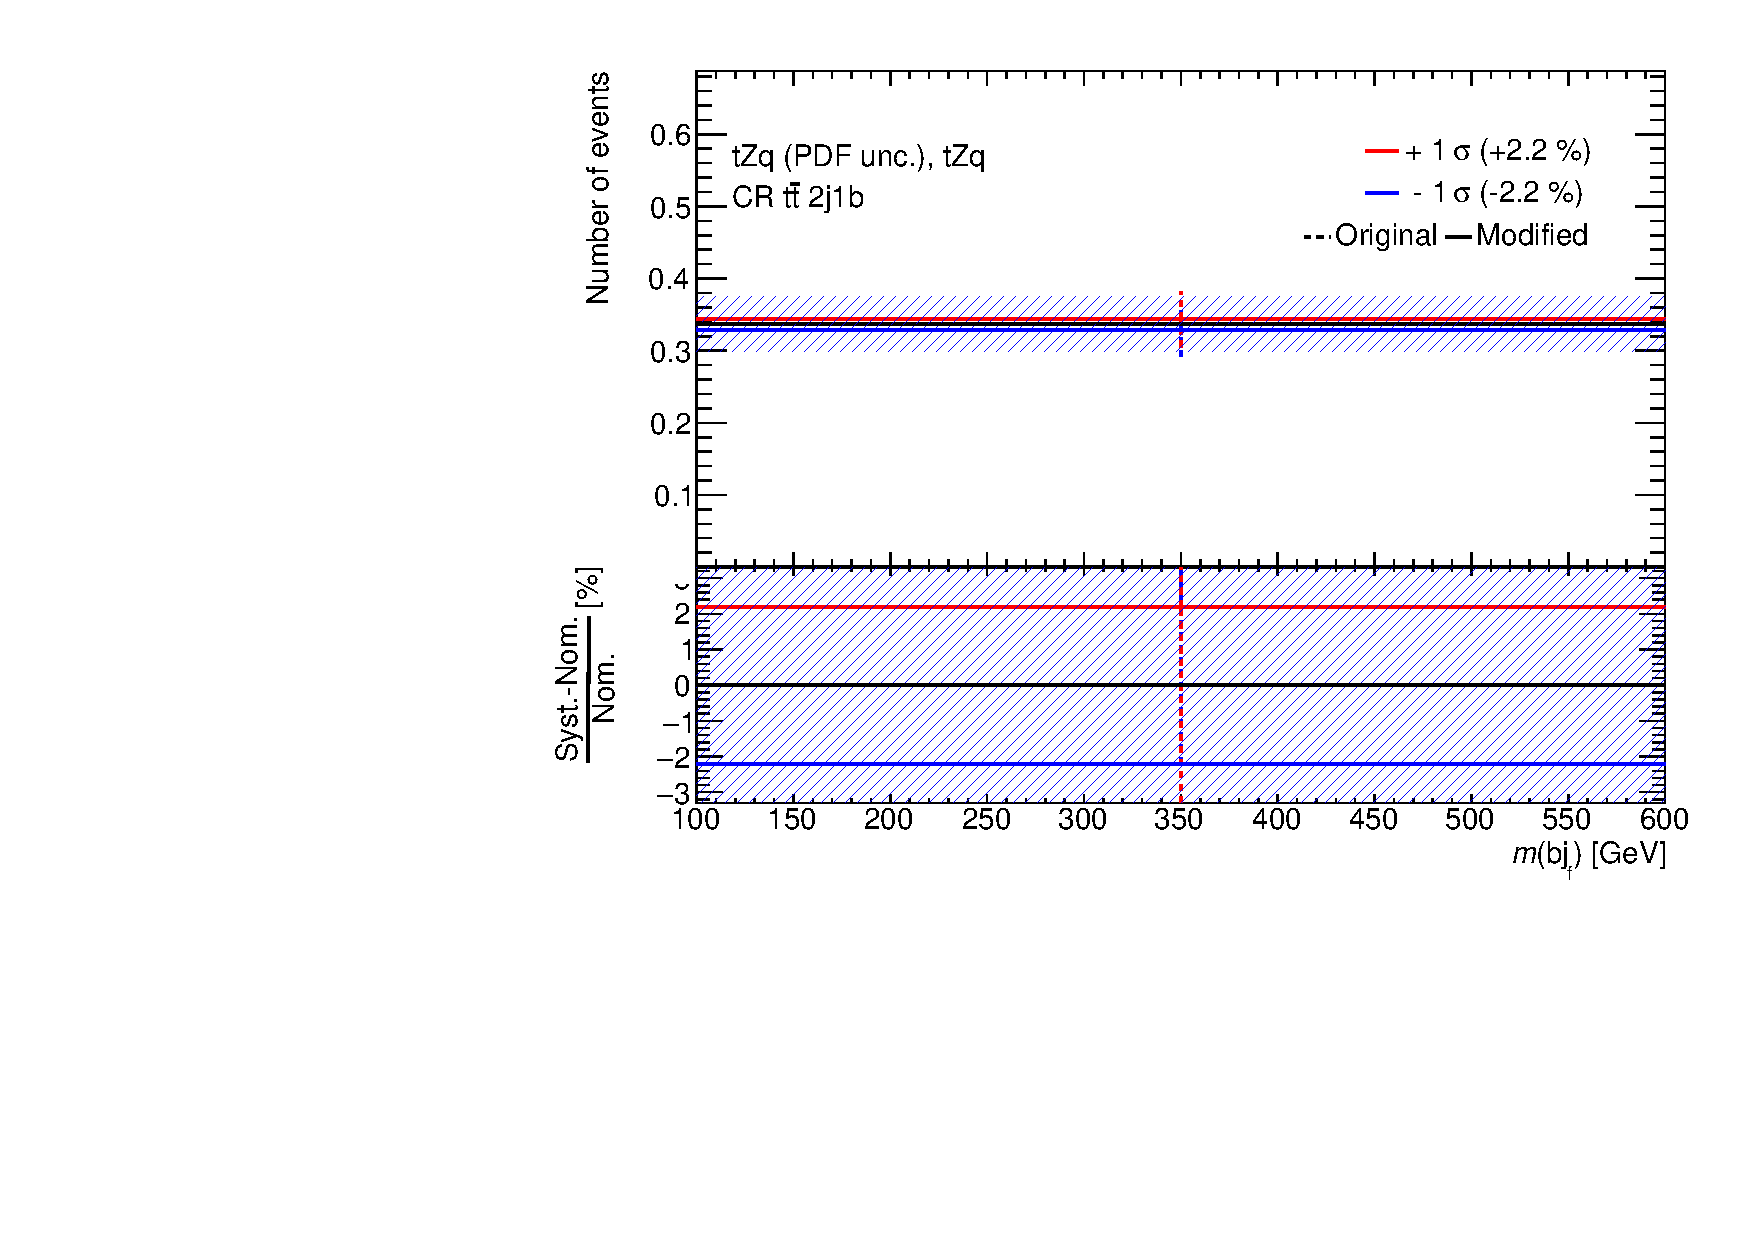
\includegraphics[width=\textwidth]{ubonn-thesis/Chapters/Chapters_07/Figure/Data/Systematic/tZq_pdf/CR_2j1b_tZq_tZq_XS_PDFunc.pdf} 
    \caption*{(g)}
  \end{subfigure} 
  \centering
  \begin{subfigure}[b]{0.33\linewidth}
    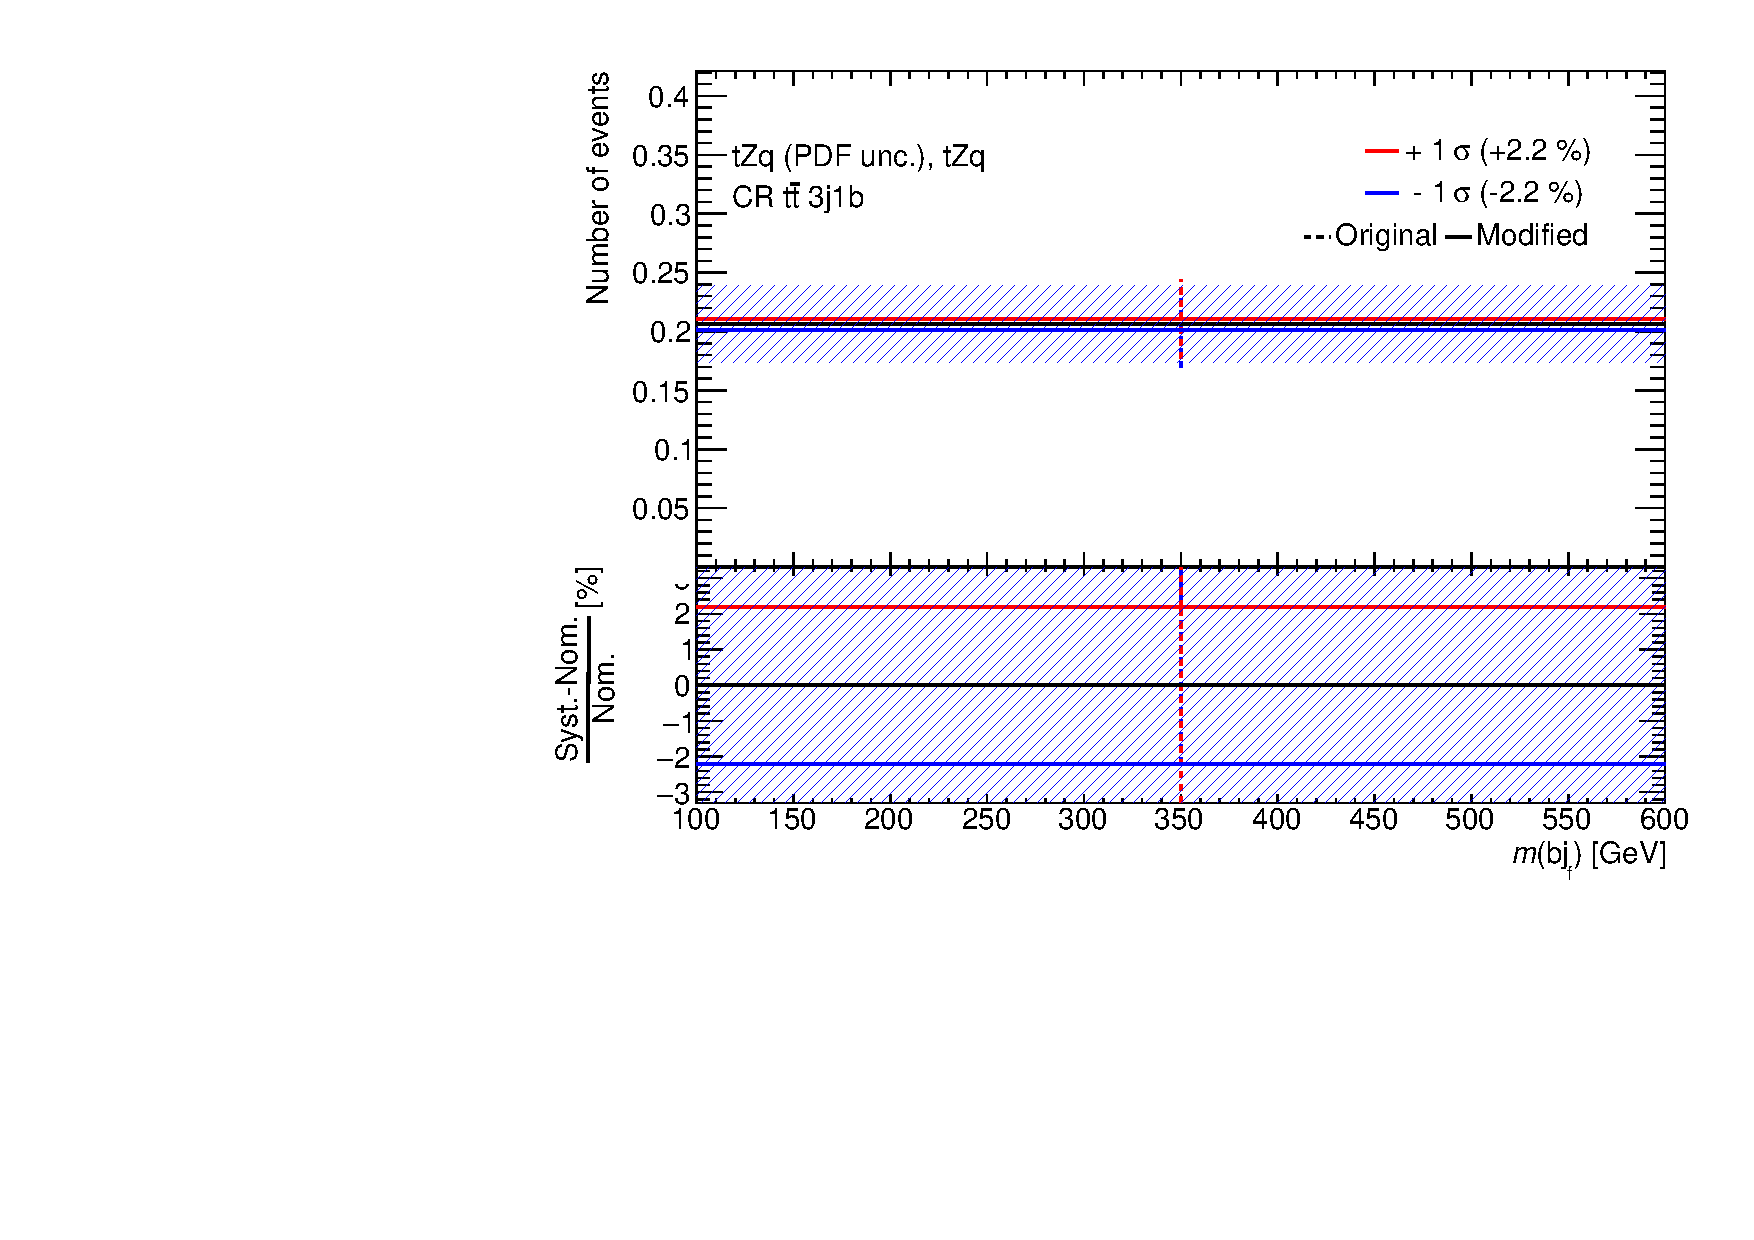
\includegraphics[width=\textwidth]{ubonn-thesis/Chapters/Chapters_07/Figure/Data/Systematic/tZq_pdf/CR_3j1b_tZq_tZq_XS_PDFunc.pdf} 
    \caption*{(h)}
  \end{subfigure}
  \caption{The effects of the tZq PDF uncert. on the total prediction in the signal and control regions. Here, lines coloured in red/blue present the $\pm 1 \sigma$ effect. The dotted/solid lines show the effect before/after smoothing, symmetrisation, and the removal of the normalisation effect (only done for shape uncertainties). The hashed bands represent the MC statistical uncertainties.}
  \label{fig:systpdf}
  \end{figure}


This is  due to constraining on NPs and anti-correlations between NPs also reduce the uncertainties. The correlation between NPs is shown in figure \ref{fig:correlation}. There is the highest anti-correlation between POI and signal uncertainties. The anti-correlation between electron uncertainties and diboson normalisation uncertainties is also high. The event yields of the pre-fit is shown in table \ref{tab:prefityield}, while the post-fit is in table \ref{tab:postfityield}. The event yields in each fitted regions for each samples give an overview of number of events before and after the fit to data.   


The impact of systematic and statistical uncertainties on the tZq cross-section, broken down into major categories is shown in table \ref{tab:impact_table}.  MC statistics refers to the effect of the limited size of the MC samples. The total systematic uncertainty is a bit larger than the quadratic sum of the individual contributions due to correlations. The uncertainties are calculated using TRExFitter framework. The pull of all NPs obtained when fitting signal regions and control regions simultaneously to the data are shown in figure \ref{fig:datapull}. It shows that only few pulls are away from zero but are still within the respective $\pm 1\sigma$ bands. The NPs with largest pull are related to signal modeling uncertainties.  The pulls are further studied to see if they are able to compensate the difference between the prediction (signal+background) and data. Therefore, histograms showing the effects of three uncertainties on the total prediction are investigated in figure \ref{fig:systQCD} and \ref{fig:systpdf}. The red and blue plots for those NPs that are either constrained or pulled. While being the highly ranked uncertainties, they have large impact on the final uncertainty as shown in table \ref{tab:impact_table}. It should be noted that, uncertainties are  dominated by the statistical uncertainties.



Finally, the measured signal strength in the observed data is $\mu = 1.30$ with a total uncertainty of 21.0\%. Here, the total uncertainty is quoted directly from the profile-likelihood fit. Multiplying the signal strength with the SM prediction $\sigma^{SM}_{t \ell^{+}\ell^{-} q}$=102 fb. the measured $t \ell^{+}\ell^{-} q$ cross-section is determined to be  132 $\pm$ 12 (stat) $\pm$ 17 (syst) fb. The statistical uncertainty is obtained by performing statonly fit as shown in figure \ref{fig:statonly}. The systematic uncertainty is then obtained by subtracting the statistical uncertainty in quadrature form from the total uncertainty. The curve obtained after performing the negative loglikelihood scan of the signal strength (POI) is shown in figure \ref{fig:dataNLL}. As in the Asimov fit, the curve is parabolic and smooth which shows that the fit is stable and results and uncertainties are reliable. The ranking of NPs is shown in figure \ref{fig:datarank}. which is very similar compared to the ranking in the Asimov fit shown in figure \ref{fig:ranking_asimov}. The relative order slightly differs because the post-fit values are different which in principle can change the impact.

\section{Discussion of the results}
\label{sec:discussionoftheresults}

The measured value of the signal strength is 1.30 $\pm$ 0.12 (stat) $\pm$ 0.17 (syst). The measurement is dominated by the systematic uncertainties. The signal uncertainty has the highest impact as shown in table \ref{tab:impact_table}. A comparison between several top quark production cross-section measurements performed in ATLAS is shown in figure \ref{fig:summarycross-section}. The rare tZq process because of its low cross-section was only measured using Run II dataset at $\sqrt{s}=13$ TeV. The measurement is performed by both ATLAS and CMS and to compare the results, a summary of both ATLAS and CMS analysis is given in table \ref{tab:summaryofATLASCMSresults}.

\begin{figure}[!h]
    \centering
    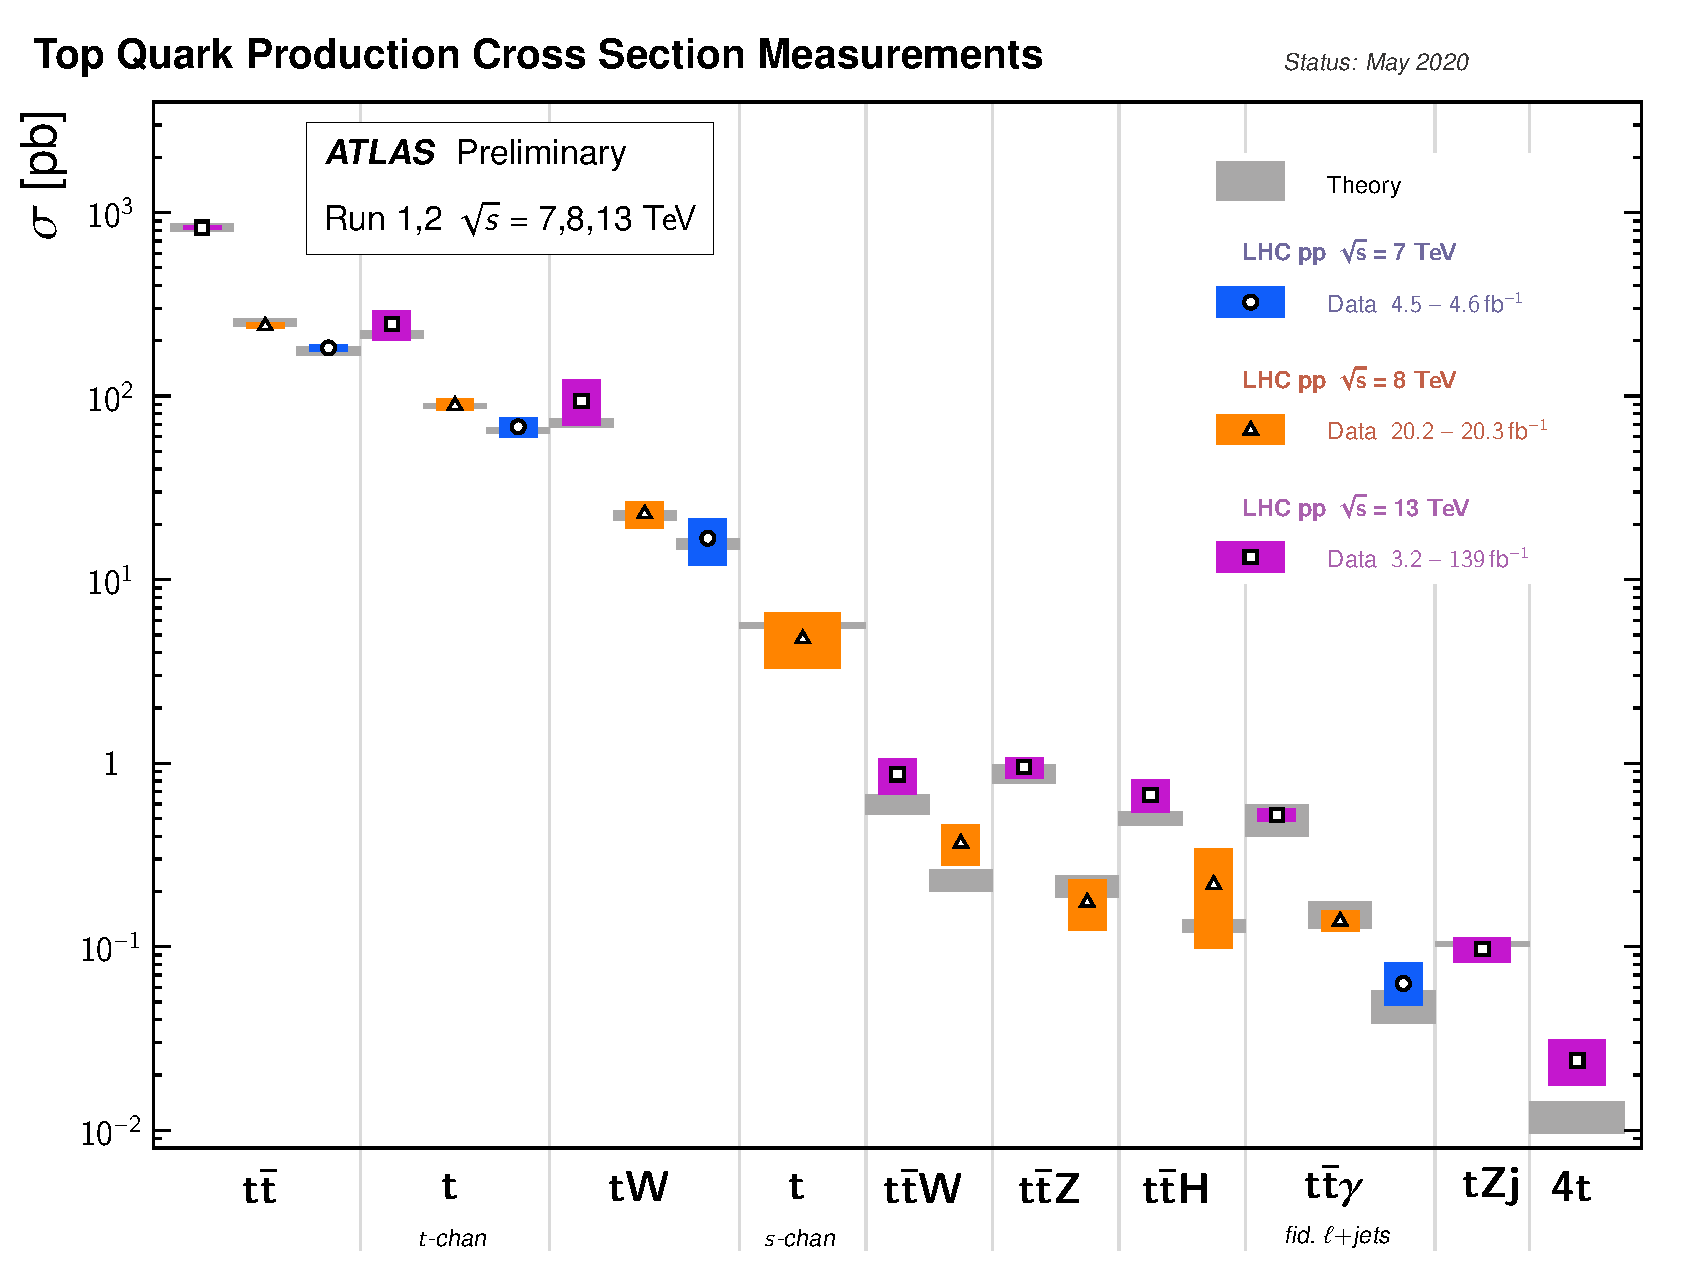
\includegraphics[width=0.85\textwidth]{ubonn-thesis/Chapters/Chapters_07/Figure/Summary_cross-section.pdf}
    \caption{Summary of several SM total production cross-section measurements at different centre-of-mass energies \cite{summarycrosssection}}
    \label{fig:summarycross-section}
\end{figure}


\begin{table}[h!]
     \centering
      \begin{tabular}{@{} *4l  @{}}
      \toprule
       & ATLAS ($t \ell^{+}\ell^{-} q$) & CMS ($t \ell^{+}\ell^{-} q$) \\
     \midrule
      $\mu$ & 0.96 & 1.18 \\[0.2ex] 
      $\sigma_{SM}(t \ell^{+}\ell^{-} q)$ & 102 fb & 94.2 \\[0.2ex] 
      $\sigma(t \ell^{+}\ell^{-} q)$ & 97 $\pm$ 13 (stat) $\pm$ 7 (syst) fb& 111 $\pm$ 13 (stat) $\pm$ 11 (syst) fb \\[0.2ex] 
      \bottomrule
 \end{tabular}
 \caption{Overview of the final results for the ATLAS ($t \ell^{+}\ell^{-} q$)cross-section and CMS ($t \ell^{+}\ell^{-} q$) measurements.}
 \label{tab:summaryofATLASCMSresults}
 \end{table}
 


The observed cross-section from ATLAS collaborations \cite{tZq2020} was  97 $\pm$ 13 (stat) $\pm$ 7 (syst) fb with an expected value of 102 fb . From the CMS collaborations  \cite{tonon2017measurement}, it was 111 $\pm$ 13 (stat) $\pm$ 11 (syst) fb with an expected value of 94 fb. The used strategy and strategies for the ATLAS and CMS measurements are similar. For separating signal and backgrounds, python based (Tensorflow, NN) MVA technique is used whereas NeuroBayes (NN) and boosted decision trees were used by ATLAS for CMS collaborations respectively. Signal extraction is done using a binned maximum likelihood fit. This analysis is different in the sense, a new frame framework is used for the analysis, new selection cuts and object definitions are used. It is important to measure the total cross-section because this framework can be used to measure the differential cross-section. The measured cross-section is higher than the recent measurements performed by ATLAS and CMS collaborations. The discrepancy in measurement can be due different signal and background event yields or the different treatment of systematic uncertainties or statistical fluctuations. The tZq QCD radaiation and PDF uncertainties have largest impact on the signal strength while uncertainties due to luminosity have largest impact on the signal strength in ATLAS analysis\cite{tZq2020}. 
